\documentclass[12pt,a4paper]{article}
\usepackage{amsmath,amssymb,mathtools}
\usepackage{geometry}
\geometry{margin=1in}
\usepackage{microtype}
\usepackage{caption}      % optional but recommended
\usepackage{subcaption} 
\usepackage{tikz}
\usetikzlibrary{arrows.meta}
\usetikzlibrary{calc}
\usetikzlibrary{angles,quotes}
\usepackage{enumitem}
\usepackage{float}
\usepackage{hyperref}
\usepackage{tikz-cd}
\usepackage{float}

\usepackage{pgfplots}
\pgfplotsset{compat=1.18}

\usetikzlibrary{positioning}

\usetikzlibrary{decorations.markings}

\usetikzlibrary{backgrounds}

\usepackage{booktabs}

\usetikzlibrary{calc,arrows.meta,patterns,decorations.pathreplacing}
\usepackage{tikz-3dplot}
\usepackage{xcolor}

\DeclareMathOperator{\ord}{ord}

\DeclareMathOperator{\Log}{Log}


\usepackage{fancyhdr}
\pagestyle{fancy}

\newcommand{\II}{\mathrm{I\!I}}

\newcommand{\C}{\mathbb{C}}

% (optional) if you also want the first fundamental form:
\newcommand{\I}{\mathrm{I}}

\newcommand{\hyp}{\mathbb{H}}

\DeclareMathOperator{\Tr}{Tr}
\newcommand{\T}{\mathsf{T}} % transpose symbol


\newcommand{\R}{\mathbb{R}}
\DeclareMathOperator{\PSL}{PSL}

\DeclareMathOperator{\Area}{Area}
\DeclareMathOperator{\Isom}{Isom}
\newcommand{\HH}{\mathbb{H}}

\newcommand{\DD}{\mathbb{D}}

\newcommand{\n}{6}

% --- codim operator (put in the preamble) ---
\DeclareMathOperator{\codim}{codim}


\newcommand{\Solution}{\par\medskip\noindent\textbf{Solution.}\ }
\newcommand{\Theory}{\par\medskip\noindent\textbf{Theory.}\ }
\newcommand{\Proof}{\par\medskip\noindent\textbf{Proof.}\ }


\fancyhf{}

\fancyfoot[C]{\thepage}

	\fancyhead[L]{\textit{Linear Algebra 1}}
\fancyhead[R]{\textit{Exercises}}

\DeclareMathOperator{\arsinh}{arsinh}

% --- HEADER ---

\usepackage{amsthm}

\theoremstyle{plain}
\newtheorem{theorem}{Theorem}[section]
\newtheorem{lemma}[theorem]{Lemma}
\newtheorem{proposition}[theorem]{Proposition}
\newtheorem{corollary}[theorem]{Corollary}

\newtheorem{definition}{Definition}

% Option A: as an operator (recommended)
\DeclareMathOperator{\Span}{span}

% or, shorter version



\newcommand{\sph}{\mathrm{sph}}


\usepackage{pgfplots}
\pgfplotsset{compat=1.18}


\theoremstyle{definition}      % bold heading, upright body
\newtheorem{example}[theorem]{Exercise}


\newtheorem*{Exercise}{Exercise}

% =========================================================
% E2 + E3  (same style as E1)
% =========================================================
% TikZ helpers (Poincaré disk geodesic from boundary angles)
% Requires: \usetikzlibrary{arrows.meta}
% =========================================================

% Draw a Poincaré disk geodesic between boundary angles a,b (degrees).
% The geodesic is the unique circle arc orthogonal to the unit circle.
% Usage: \DiskGeodesic[<draw options>]{<a deg>}{<b deg>}
% Robust Poincaré disk geodesic between boundary angles a,b (degrees).
% Handles the diameter case (antipodal endpoints) where det=0.
% Robust Poincaré disk geodesic between boundary angles a,b (degrees).
\newcommand{\DiskGeodesic}[3][]{%
	\pgfmathsetmacro{\ax}{cos(#2)}%
	\pgfmathsetmacro{\ay}{sin(#2)}%
	\pgfmathsetmacro{\bx}{cos(#3)}%
	\pgfmathsetmacro{\by}{sin(#3)}%
	
	% det = ax*by - ay*bx
	\pgfmathsetmacro{\det}{\ax*\by - \ay*\bx}%
	\pgfmathsetmacro{\detabs}{abs(\det)}%
	
	% diameter / antipodal case: det ~ 0
	\ifdim \detabs pt < 0.000001pt
	\draw[#1] (\ax,\ay) -- (\bx,\by);
	\else
	\pgfmathsetmacro{\h}{(\by-\ay)/\det}%
	\pgfmathsetmacro{\k}{(\ax-\bx)/\det}%
	\pgfmathsetmacro{\Rgeo}{sqrt(\h*\h+\k*\k-1)}%
	\pgfmathsetmacro{\tA}{atan2(\ay-\k,\ax-\h)}%
	\pgfmathsetmacro{\tB}{atan2(\by-\k,\bx-\h)}%
	\pgfmathsetmacro{\dAB}{\tB-\tA}%
	\pgfmathsetmacro{\dAB}{ifthenelse(\dAB>180,\dAB-360,\dAB)}%
	\pgfmathsetmacro{\dAB}{ifthenelse(\dAB<-180,\dAB+360,\dAB)}%
	\pgfmathsetmacro{\tEnd}{\tA+\dAB}%
	\draw[#1] (\h,\k) ++(\tA:\Rgeo)
	arc[start angle=\tA, end angle=\tEnd, radius=\Rgeo];
	\fi
}

% --- palette ---
\definecolor{BBlue}{RGB}{0,92,184}
\definecolor{GOrange}{RGB}{230,120,20}
\definecolor{PGreen}{RGB}{0,140,90}
\definecolor{RRed}{RGB}{200,40,60}
\definecolor{LFill}{RGB}{240,245,255}

% --- tikz styles ---
\tikzset{
	base/.style={thick, draw=black!65},
	gamma/.style={very thick, draw=GOrange, -{Latex[length=2.2mm]}},
	fiber/.style={thick, draw=BBlue},
	section/.style={thick, draw=PGreen},
	transport/.style={very thick, draw=RRed, -{Latex[length=2.2mm]}},
	pt/.style={circle, fill=black, inner sep=1.3pt},
	spt/.style={circle, fill=PGreen, inner sep=1.3pt},
	lab/.style={fill=white, fill opacity=1, text opacity=1, inner sep=2pt, rounded corners=2pt}
}


\newtheorem{remark}[theorem]{Remark} 
\tikzset{
	>={Latex[length=2.6mm]},
	axis/.style={black, thin, ->},
	unitcircle/.style={black, very thin},
	pole/.style={red!70!black, fill=red!70!black},
	polemark/.style={red!70!black, thick},
	removable/.style={black, thick},
	essstar/.style={yellow!65!orange, star, star points=7, minimum size=6pt, draw=orange!80!black, fill=yellow!70!orange},
	lattice/.style={blue!70!black, fill=blue!70!black},
	note/.style={black!70, font=\scriptsize}
}
\usetikzlibrary{arrows.meta,shapes.geometric}

% --- colors and styles for the charts ---
\definecolor{PoleRed}{RGB}{214,49,56}
\definecolor{SimpleBlue}{RGB}{31,119,180}
\definecolor{Gold}{RGB}{247,183,51}

% styles
\definecolor{PoleRed}{RGB}{214,49,56}
\tikzset{
	>={Latex[length=3.4mm]},
	axis/.style={black, line width=1.0pt, ->},
	pole2/.style={PoleRed, line width=1.8pt},
	removable/.style={black, line width=1.6pt},
	leader/.style={black!70, line width=0.9pt},
	labelfunc/.style={font=\large},
	labeltext/.style={black!85, font=\normalsize},
	callout/.style={
		draw=black!40, fill=white, rounded corners=3pt,
		inner sep=5pt, outer sep=5pt,
		text=black, opacity=1, text opacity=1  % <- force visible text
	},
}


\tikzset{
	->-/.style={
		postaction={decorate},
		decoration={
			markings,
			mark=at position 0.18 with {\arrow{Stealth[length=2.2mm]}}
		}
	},
	% p10loop must NOT use "expanded"
	p10loop/.style={thick}
}



% --- colors (define what you use) ---
\definecolor{DiagBlue}{RGB}{0,92,184}
\definecolor{DiagOrange}{RGB}{230,120,20}
\definecolor{DiagGreen}{RGB}{0,140,90}
\definecolor{DiagRed}{RGB}{200,40,60}
\definecolor{DiagGray}{RGB}{80,80,80}
\definecolor{DiagLight}{RGB}{240,245,255} % <-- this fixes \fill[DiagLight]...

% --- tikz styles (define what you use in [ax], [base], [fib], [pt2], [lab], etc.) ---
\tikzset{
	ax/.style={-{Latex[length=2.2mm]}, thick, draw=DiagGray},
	base/.style={thick, draw=DiagBlue},
	fib/.style={thick, draw=DiagGray},
	loop/.style={-{Latex[length=2.2mm]}, very thick, draw=DiagOrange},
	transport/.style={-{Latex[length=2.2mm]}, very thick, draw=DiagRed},
	pt/.style={circle, fill=DiagRed, inner sep=1.2pt},
	pt2/.style={circle, fill=DiagGreen, inner sep=1.2pt},
	lab/.style={fill=white, fill opacity=1, text opacity=1,
		inner sep=2.2pt, rounded corners=2pt}
}

\title{Linear Algebra 1}
\author{}
\date{}




\begin{document}
	\maketitle

\subsection*{Problem Set — Bases, Subspaces, and Vector-Space Isomorphisms}

\subsubsection*{Problem 1 — Which modified lists are bases?}

\textbf{Exact statement.}
Suppose that the vectors $e_1,\dots,e_n$ form a basis for a real vector space $V$.
Which of the following are also bases?
\begin{enumerate}
	\item[(a)] $e_1+e_2,\ e_2+e_3,\ \dots,\ e_{n-1}+e_n,\ e_n$;
	\item[(b)] $e_1+e_2,\ e_2+e_3,\ \dots,\ e_{n-1}+e_n,\ e_n+e_1$;
	\item[(c)] $e_1-e_n,\ e_2+e_{n-1},\ \dots,\ e_n+(-1)^n e_1$.
\end{enumerate}

\textbf{Solution.}
Write the proposed lists as $v_1,\dots,v_n$.

\medskip
\noindent\textbf{(a)} Let $v_k=e_k+e_{k+1}$ for $1\le k\le n-1$ and $v_n=e_n$.
Then we can recover the original basis:
\[
e_n=v_n,\qquad
e_{n-1}=v_{n-1}-e_n,\qquad
e_{n-2}=v_{n-2}-e_{n-1},\ \dots,\ 
e_1=v_1-e_2.
\]
Hence $v_1,\dots,v_n$ span $V$ and are linearly independent; they form a basis.

\medskip
\noindent\textbf{(b)} Let $v_k=e_k+e_{k+1}$ for $1\le k\le n-1$ and $v_n=e_n+e_1$.
Consider the alternating sum
\[
S:=v_1-v_2+v_3-\cdots+(-1)^{n-1}v_n.
\]
A direct cancellation shows:
\[
S=
\begin{cases}
	0, & n\ \text{even},\\[4pt]
	2e_1, & n\ \text{odd}.
\end{cases}
\]
If $n$ is even, this gives a nontrivial linear dependence, so the list is not a basis.
If $n$ is odd, then $e_1=\tfrac12 S$ lies in $\mathrm{span}(v_1,\dots,v_n)$, and then
\[
e_2=v_1-e_1,\quad e_3=v_2-e_2,\quad \dots,\quad e_n=v_{n-1}-e_{n-1},
\]
so all $e_i$ lie in the span; hence $v_1,\dots,v_n$ span $V$. Since there are $n$ vectors spanning an
$n$-dimensional space, they form a basis. Therefore (b) is a basis iff $n$ is odd.

\medskip
\noindent\textbf{(c)} Interpret the pattern as
\[
v_k:=e_k+(-1)^k e_{n+1-k}\qquad (1\le k\le n).
\]
Pair indices $k$ and $m:=n+1-k$. Then
\[
v_k=e_k+(-1)^k e_m,\qquad
v_m=e_m+(-1)^m e_k.
\]
If $n$ is odd, then $(-1)^m=(-1)^{n+1-k}=(-1)^{n+1}(-1)^k=(+1)(-1)^k=(-1)^k$, so
\[
v_k-(-1)^k v_m = 0
\]
for each pair, giving a nontrivial dependence; hence not a basis.

If $n$ is even, then $(-1)^m=(-1)^{n+1-k}=(-1)^{n+1}(-1)^k=-( -1)^k$, so
\[
v_k=e_k+s e_m,\qquad v_m=e_m-s e_k,\qquad (s:=(-1)^k).
\]
Solving yields
\[
e_k=\frac{v_k-sv_m}{2},\qquad e_m=\frac{sv_k+v_m}{2}.
\]
Thus every $e_i$ lies in $\mathrm{span}(v_1,\dots,v_n)$, so the $v_i$ span $V$ and hence form a basis.
Therefore (c) is a basis iff $n$ is even.

\bigskip

\subsubsection*{Problem 2 — Unions and distributive-looking identities}

\textbf{Exact statement.}
Let $T,U,W$ be subspaces of $V$.
\begin{enumerate}
	\item[(i)] Show that $T\cup U$ is a subspace of $V$ only if either $T\subseteq U$ or $U\subseteq T$.
	\item[(ii)] Give explicit counterexamples to:
	\begin{enumerate}
		\item[(a)] $T+(U\cap W)=(T+U)\cap(T+W)$;
		\item[(b)] $(T+U)\cap W=(T\cap W)+(U\cap W)$.
	\end{enumerate}
	\item[(iii)] Show that each equality in (ii) can be replaced by a valid inclusion of one side in the other.
\end{enumerate}

\textbf{Solution.}
\textbf{(i)} If $T\subseteq U$ or $U\subseteq T$, then $T\cup U$ equals the larger subspace, hence is a subspace.
Conversely, assume $T\cup U$ is a subspace and neither contains the other.
Choose $t\in T\setminus U$ and $u\in U\setminus T$. Since $T\cup U$ is a subspace, it is closed under addition,
so $t+u\in T\cup U$. If $t+u\in T$, then $u=(t+u)-t\in T$, contradiction. If $t+u\in U$, then
$t=(t+u)-u\in U$, contradiction. Hence one must contain the other.

\medskip
\textbf{(ii)(a)} In $V=\mathbb R^2$, let
\[
T=\mathrm{span}(e_1),\qquad U=\mathrm{span}(e_2),\qquad W=\mathrm{span}(e_1+e_2).
\]
Then $U\cap W=\{0\}$, so $T+(U\cap W)=T$. But $T+U=\mathbb R^2$ and $T+W=\mathbb R^2$, hence
\[
(T+U)\cap(T+W)=\mathbb R^2\neq T.
\]

\medskip
\textbf{(ii)(b)} In $V=\mathbb R^2$, let
\[
T=\mathrm{span}(e_1+e_2),\qquad U=\mathrm{span}(e_1-e_2),\qquad W=\mathrm{span}(e_1).
\]
Then $T+U=\mathbb R^2$, so $(T+U)\cap W=W$. But $T\cap W=\{0\}$ and $U\cap W=\{0\}$, so
\[
(T\cap W)+(U\cap W)=\{0\}\neq W.
\]

\medskip
\textbf{(iii)} For (a), if $x\in T+(U\cap W)$ then $x=t+z$ with $t\in T$ and $z\in U\cap W$.
Thus $x\in T+U$ and $x\in T+W$, so
\[
T+(U\cap W)\subseteq (T+U)\cap(T+W).
\]
For (b), if $x\in (T\cap W)+(U\cap W)$ then $x=t+u$ with $t\in T\cap W$ and $u\in U\cap W$.
Then $t,u\in W$ so $x\in W$, and also $t\in T$, $u\in U$ so $x\in T+U$. Hence
\[
(T\cap W)+(U\cap W)\subseteq (T+U)\cap W.
\]

\bigskip

\subsubsection*{Problem 3 — Decide if $V\cong W$ and exhibit an isomorphism if so}

\textbf{Exact statement.}
For each pair $(V,W)$ of vector spaces over $\mathbb R$, either give an isomorphism $V\to W$
or show that no such isomorphism can exist. Here $P(\mathbb R)$ denotes polynomial functions $\mathbb R\to\mathbb R$
and $C[a,b]$ denotes continuous real-valued functions on $[a,b]$.
\begin{enumerate}
	\item[(a)] $V=\mathbb R^4$, $W=\{x\in\mathbb R^5:\ x_1+x_2+x_3+x_4+x_5=0\}$.
	\item[(b)] $V=\mathbb R^5$, $W=\{p\in P:\ \deg p\le 5\}$.
	\item[(c)] $V=C[0,1]$, $W=C[-1,1]$.
	\item[(d)] $V=C[0,1]$, $W=\{f\in C[0,1]: f(0)=0,\ f\text{ continuously differentiable}\}$.
	\item[(e)] $V=\mathbb R^2$, $W=\{\text{real solutions of } \ddot x(t)+x(t)=0\}$.
	\item[(f)] $V=\mathbb R^4$, $W=C[0,1]$.
	\item[(g)] (Harder) $V=P(\mathbb R)$, $W=\mathbb R^{\mathbb N}$.
\end{enumerate}

\textbf{Solution.}

\medskip
\noindent\textbf{(a)} Define
\[
\phi:\mathbb R^4\to W,\qquad \phi(a,b,c,d)=(a,b,c,d,-(a+b+c+d)).
\]
Then $\phi$ is linear, injective, and surjective (projection onto the first four coordinates is an inverse).
Hence $V\cong W$.

\medskip
\noindent\textbf{(b)} $W$ has basis $\{1,x,x^2,x^3,x^4,x^5\}$, so $\dim W=6$, while $\dim\mathbb R^5=5$.
Thus no isomorphism exists.

\medskip
\noindent\textbf{(c)} Let $\alpha:[-1,1]\to[0,1]$ be $\alpha(t)=\frac{t+1}{2}$.
Define
\[
F:C[0,1]\to C[-1,1],\qquad (Ff)(t)=f(\alpha(t)).
\]
Then $F$ is linear and bijective with inverse
\[
(F^{-1}g)(x)=g(2x-1).
\]
Hence $C[0,1]\cong C[-1,1]$.

\medskip
\noindent\textbf{(d)} Define
\[
T:C[0,1]\to W,\qquad (Tf)(x)=\int_0^x f(t)\,dt.
\]
Then $Tf\in C^1[0,1]$, $(Tf)(0)=0$, and $(Tf)'=f$. Thus $T$ is linear.
If $Tf=0$, then differentiating gives $f=0$, so $T$ is injective. If $g\in W$, then $g'=h\in C[0,1]$ and
\[
g(x)=g(0)+\int_0^x g'(t)\,dt=\int_0^x h(t)\,dt = Th(x),
\]
so $T$ is surjective. Hence $V\cong W$ with inverse $g\mapsto g'$.

\medskip
\noindent\textbf{(e)} The solution set of $\ddot x + x=0$ is
\[
W=\{\,x(t)=a\cos t + b\sin t:\ a,b\in\mathbb R\,\}.
\]
Define
\[
\psi:\mathbb R^2\to W,\qquad \psi(a,b)(t)=a\cos t+b\sin t.
\]
This map is linear and bijective, so $V\cong W$.

\medskip
\noindent\textbf{(f)} $\mathbb R^4$ is finite-dimensional.
But $C[0,1]$ is infinite-dimensional since $\{1,x,x^2,\dots\}$ is linearly independent in $C[0,1]$.
Therefore no isomorphism exists.

\medskip
\noindent\textbf{(g)} $P(\mathbb R)$ has countable basis $\{1,x,x^2,\dots\}$, hence $\dim P(\mathbb R)=\aleph_0$.
In $\mathbb R^{\mathbb N}$, for each $r\in\mathbb R$ define
\[
v_r:=(1,r,r^2,r^3,\dots).
\]
If $r_1,\dots,r_k$ are distinct and $\sum_{i=1}^k a_i v_{r_i}=0$, then looking at coordinates $n=0,1,\dots,k-1$ gives
\[
\sum_{i=1}^k a_i r_i^n=0\qquad (n=0,1,\dots,k-1),
\]
a Vandermonde system with nonzero determinant, forcing $a_i=0$ for all $i$.
Thus $\{v_r:r\in\mathbb R\}$ is linearly independent, so $\dim(\mathbb R^{\mathbb N})\ge |\mathbb R|$.
Since $|\mathbb R^{\mathbb N}|=|\mathbb R|$, we get $\dim(\mathbb R^{\mathbb N})=|\mathbb R|$ (uncountable).
Hence $P(\mathbb R)\not\cong \mathbb R^{\mathbb N}$.

\subsection*{Theory — Bases, Subspaces, and Isomorphisms (for Problems 1--3)}

\subsubsection*{A. Bases and change-of-basis matrices}

Let $(e_1,\dots,e_n)$ be a basis of a real vector space $V$.
Given vectors $(v_1,\dots,v_n)$ in $V$, write each $v_j$ uniquely as
\[
v_j=\sum_{i=1}^n a_{ij} e_i.
\]
The coefficient matrix $A=(a_{ij})$ is the change-of-coordinates matrix from the $e$-basis to the $v$-list.

\medskip
\noindent\textbf{Basis criterion.}
The following are equivalent:
\[
(v_1,\dots,v_n)\ \text{is a basis}
\quad\Longleftrightarrow\quad
\text{columns of }A\text{ are linearly independent}
\quad\Longleftrightarrow\quad
A\text{ is invertible}
\quad\Longleftrightarrow\quad
\det(A)\neq 0.
\]

\medskip
\noindent\textbf{Triangular case.}
If $A$ is triangular (upper or lower), then
\[
\det(A)=\prod_{i=1}^n a_{ii}.
\]
Hence a triangular $A$ with all diagonal entries nonzero is automatically invertible. In practice this corresponds
to solving for the original basis vectors by back-substitution.

\bigskip

\subsubsection*{B. Subspaces: unions, sums, intersections, and inclusions}

\noindent\textbf{Subspace test.}
A nonempty subset $S\subseteq V$ is a subspace iff it is closed under addition and scalar multiplication.

\medskip
\noindent\textbf{Union of subspaces.}
If $T$ and $U$ are subspaces, then $T\cup U$ is a subspace only in the nested case:
\[
T\cup U\ \text{is a subspace}\quad\Longleftrightarrow\quad T\subseteq U\ \text{or}\ U\subseteq T.
\]
Indeed, if $t\in T\setminus U$ and $u\in U\setminus T$, then $t+u$ cannot lie in $T$ or $U$ (otherwise subtraction
would force containment), contradicting closure under addition.

\medskip
\noindent\textbf{Sum and intersection.}
For subspaces $T,U\le V$,
\[
T+U:=\{t+u:\ t\in T,\ u\in U\}
\]
is the smallest subspace containing $T$ and $U$, and $T\cap U$ is always a subspace.

\medskip
\noindent\textbf{Always-true inclusions.}
For any subspaces $T,U,W\le V$,
\[
T+(U\cap W)\subseteq (T+U)\cap(T+W).
\]
(If $x=t+z$ with $z\in U\cap W$, then $x\in T+U$ and $x\in T+W$.)
Also,
\[
(T\cap W)+(U\cap W)\subseteq (T+U)\cap W.
\]
(Each summand lies in $W$ and in $T+U$.)

\medskip
\noindent\textbf{Modular law (useful sufficient condition for equality).}
If $T\subseteq W$, then
\[
T+(U\cap W)=(T+U)\cap W.
\]
Thus ``distributive-like'' equalities may fail without extra containment hypotheses, but inclusions remain valid.

\medskip
\noindent\textbf{Grassmann formula (finite-dimensional $V$).}
If $V$ is finite-dimensional and $T,U\le V$, then
\[
\dim(T+U)=\dim T+\dim U-\dim(T\cap U).
\]

\bigskip

\subsubsection*{C. Vector-space isomorphisms}

\noindent\textbf{Definition.}
A linear map $L:V\to W$ is an isomorphism if it is bijective (equivalently, has a linear inverse).

\medskip
\noindent\textbf{Finite-dimensional classification.}
If $V$ and $W$ are finite-dimensional over $\mathbb R$, then
\[
V\cong W \quad\Longleftrightarrow\quad \dim V=\dim W.
\]
Given bases $(v_i)$ of $V$ and $(w_i)$ of $W$, the map $L(v_i)=w_i$ extends uniquely to an isomorphism.

\medskip
\noindent\textbf{Standard dimension facts.}
A single nontrivial linear equation in $\mathbb R^n$ defines a hyperplane of dimension $n-1$.
Polynomials of degree $\le m$ have basis $\{1,x,\dots,x^m\}$ and hence dimension $m+1$.

\medskip
\noindent\textbf{Function spaces via reparametrization.}
If $\alpha:[c,d]\to[a,b]$ is a homeomorphism, then
\[
C[a,b]\cong C[c,d],\qquad f\mapsto f\circ \alpha.
\]
In suitable settings, integration/differentiation can yield isomorphisms, e.g.
\[
C[0,1]\to \{g\in C^1[0,1]:g(0)=0\},\qquad f\mapsto\Big(x\mapsto\int_0^x f(t)\,dt\Big).
\]

\medskip
\noindent\textbf{Linear ODE solution spaces.}
For a linear homogeneous ODE of order $k$, the space of real solutions is a $k$-dimensional real vector space.
For $\ddot x + x=0$, a basis is $\{\cos t,\sin t\}$.

\medskip
\noindent\textbf{Infinite-dimensional obstructions.}
A finite-dimensional vector space is never isomorphic to an infinite-dimensional one.
Moreover, $P(\mathbb R)$ has a countable basis $\{1,x,x^2,\dots\}$, while $\mathbb R^{\mathbb N}$ has uncountable
Hamel dimension (one can exhibit a continuum-sized linearly independent set via a Vandermonde argument).
Therefore $P(\mathbb R)\not\cong \mathbb R^{\mathbb N}$.


\subsubsection*{Problem 4 — Sum of linear maps; images/kernels; idempotents}

\textbf{Exact statement.}
\begin{enumerate}
	\item[(i)] If $\alpha$ and $\beta$ are linear maps from $U$ to $V$ show that $\alpha+\beta$ is linear.
	Give explicit counter-examples to:
	\[
	\text{(a) }\operatorname{im}(\alpha+\beta)=\operatorname{im}(\alpha)+\operatorname{im}(\beta),\qquad
	\text{(b) }\ker(\alpha+\beta)=\ker(\alpha)\cap\ker(\beta).
	\]
	Show that in general each equality can be replaced by a valid inclusion of one side in the other.
	\item[(ii)] Let $\alpha:V\to V$ be linear. Show that if $\alpha^2=\alpha$ then
	$V=\ker(\alpha)\oplus \operatorname{im}(\alpha)$.
	Does your proof still work if $V$ is infinite dimensional? Is the result still true?
\end{enumerate}

\textbf{Solution.}
\textbf{(i)} For $u,u'\in U$ and $\lambda\in\mathbb R$,
\[
(\alpha+\beta)(u+u')=\alpha(u+u')+\beta(u+u')
=(\alpha u+\alpha u')+(\beta u+\beta u')
=(\alpha+\beta)u+(\alpha+\beta)u',
\]
\[
(\alpha+\beta)(\lambda u)=\alpha(\lambda u)+\beta(\lambda u)=\lambda\alpha(u)+\lambda\beta(u)
=\lambda(\alpha+\beta)(u),
\]
so $\alpha+\beta$ is linear.

Counterexample to (a): take $U=V=\mathbb R$, $\alpha=\mathrm{id}$, $\beta=-\mathrm{id}$.
Then $\alpha+\beta=0$, hence $\operatorname{im}(\alpha+\beta)=\{0\}$ but
$\operatorname{im}(\alpha)+\operatorname{im}(\beta)=\mathbb R$.
In general,
\[
\operatorname{im}(\alpha+\beta)\subseteq \operatorname{im}(\alpha)+\operatorname{im}(\beta),
\]
since $(\alpha+\beta)(u)=\alpha(u)+\beta(u)$.

Counterexample to (b): with the same $\alpha,\beta$, we have $\ker(\alpha+\beta)=\mathbb R$ but
$\ker(\alpha)\cap\ker(\beta)=\{0\}$.
In general,
\[
\ker(\alpha)\cap\ker(\beta)\subseteq \ker(\alpha+\beta),
\]
since $\alpha(u)=\beta(u)=0\Rightarrow (\alpha+\beta)(u)=0$.

\medskip
\textbf{(ii)} Assume $\alpha^2=\alpha$.
For any $x\in V$,
\[
x=(x-\alpha x)+\alpha x.
\]
Moreover,
\[
\alpha(x-\alpha x)=\alpha x-\alpha^2 x=\alpha x-\alpha x=0,
\]
so $x-\alpha x\in\ker(\alpha)$ and $\alpha x\in\operatorname{im}(\alpha)$, hence
$V=\ker(\alpha)+\operatorname{im}(\alpha)$.

If $y\in\ker(\alpha)\cap\operatorname{im}(\alpha)$, then $y=\alpha(x)$ for some $x$ and
$0=\alpha(y)=\alpha(\alpha x)=\alpha^2 x=\alpha x=y$, so $y=0$. Thus the sum is direct:
\[
V=\ker(\alpha)\oplus\operatorname{im}(\alpha).
\]
No finite-dimensional hypothesis was used, so the proof works for infinite-dimensional $V$ and the result remains true.

\bigskip

\subsubsection*{Problem 5 — Bases for $U$, $W$, $U\cap W$, and a description of $U+W$ in $\mathbb R^5$}

\textbf{Exact statement.}
Let
\[
U=\{x\in\mathbb R^5:\ x_1+x_3+x_4=0,\ \ 2x_1+2x_2+x_5=0\},\qquad
W=\{x\in\mathbb R^5:\ x_1+x_5=0,\ \ x_2=x_3=x_4\}.
\]
Find bases for $U$ and $W$ containing a basis for $U\cap W$ as a subset.
Give a basis for $U+W$ and show that
\[
U+W=\{x\in\mathbb R^5:\ x_1+2x_2+x_5=x_3+x_4\}.
\]

\textbf{Solution.}
For $U$, solve
\[
x_1=-x_3-x_4,\qquad x_5=-2x_1-2x_2=2x_3+2x_4-2x_2.
\]
With free variables $x_2,x_3,x_4$,
\[
x=x_2(0,1,0,0,-2)+x_3(-1,0,1,0,2)+x_4(-1,0,0,1,2).
\]
Thus a basis of $U$ is
\[
u_1=(0,1,0,0,-2),\quad u_2=(-1,0,1,0,2),\quad u_3=(-1,0,0,1,2).
\]

For $W$, write $x_2=x_3=x_4=t$ and $x_1=s$, so $x_5=-s$. Then
\[
x=(s,t,t,t,-s)=s(1,0,0,0,-1)+t(0,1,1,1,0),
\]
hence a basis of $W$ is
\[
w_1=(1,0,0,0,-1),\quad w_2=(0,1,1,1,0).
\]

For $U\cap W$, take $x=(s,t,t,t,-s)\in W$ and impose $x_1+x_3+x_4=0$:
\[
s+2t=0\Rightarrow s=-2t.
\]
Therefore
\[
U\cap W=\mathrm{span}\{v\},\qquad v=(-2,1,1,1,2).
\]
Note that $v=u_1+u_2+u_3$ and $v=-2w_1+w_2$, so bases containing $v$ are
\[
\mathcal B_U=\{v,u_2,u_3\}\ \text{ for }U,\qquad \mathcal B_W=\{v,w_1\}\ \text{ for }W.
\]
Since $\dim(U+W)=3+2-1=4$, a basis for $U+W$ is
\[
\mathcal B_{U+W}=\{v,u_2,u_3,w_1\}.
\]

Let $S:=\{x\in\mathbb R^5:\ x_1+2x_2+x_5=x_3+x_4\}$.
If $x\in U+W$ and $x=a v+b u_2+c u_3+d w_1$, then a coordinate check gives
$x_1+2x_2+x_5=x_3+x_4$, hence $U+W\subseteq S$.

Conversely, given $x\in S$, set
\[
a=x_2,\qquad b=x_3-x_2,\qquad c=x_4-x_2,\qquad d=x_1+x_3+x_4.
\]
Then one verifies $x=a v+b u_2+c u_3+d w_1$, hence $x\in U+W$, so $S\subseteq U+W$.
Therefore $U+W=S$.

\bigskip

\subsubsection*{Problem 6 — Descending images, ascending kernels, and rank constraints}

\textbf{Exact statement.}
\begin{enumerate}
	\item[(i)] Let $\alpha:V\to V$ be an endomorphism of a finite dimensional vector space $V$.
	Show that
	\[
	V\supseteq \operatorname{im}(\alpha)\supseteq \operatorname{im}(\alpha^2)\supseteq \cdots,\qquad
	\{0\}\subseteq \ker(\alpha)\subseteq \ker(\alpha^2)\subseteq \cdots.
	\]
	If $r_k=\mathrm{rk}(\alpha^k)$, deduce that $r_k\ge r_{k+1}$ and
	$r_k-r_{k+1}\ge r_{k+1}-r_{k+2}$.
	Conclude that if for some $k\ge 0$ we have $r_k=r_{k+1}$, then $r_k=r_{k+\ell}$ for all $\ell\ge 0$.
	\item[(ii)] Suppose $\dim(V)=5$, $\alpha^3=0$, but $\alpha^2\ne 0$.
	What possibilities are there for $\mathrm{rk}(\alpha)$ and $\mathrm{rk}(\alpha^2)$?
\end{enumerate}

\textbf{Solution.}
\textbf{(i)} Since
\[
\operatorname{im}(\alpha^{k+1})=\alpha(\operatorname{im}(\alpha^k))\subseteq \operatorname{im}(\alpha^k),
\]
the images form a descending chain. Also $\alpha^k(v)=0\Rightarrow \alpha^{k+1}(v)=\alpha(0)=0$, hence
$\ker(\alpha^k)\subseteq \ker(\alpha^{k+1})$.

Let $r_k=\dim\operatorname{im}(\alpha^k)$. The inclusion
$\operatorname{im}(\alpha^{k+1})\subseteq \operatorname{im}(\alpha^k)$ implies $r_k\ge r_{k+1}$.

Consider the restriction $\alpha:\operatorname{im}(\alpha^k)\to \operatorname{im}(\alpha^{k+1})$, which is surjective.
Rank--nullity for this restricted map gives
\[
\dim(\ker(\alpha)\cap \operatorname{im}(\alpha^k))
=\dim\operatorname{im}(\alpha^k)-\dim\operatorname{im}(\alpha^{k+1})
=r_k-r_{k+1}.
\]
Similarly,
\[
r_{k+1}-r_{k+2}=\dim(\ker(\alpha)\cap \operatorname{im}(\alpha^{k+1})).
\]
Since $\operatorname{im}(\alpha^{k+1})\subseteq \operatorname{im}(\alpha^k)$, we have
\[
\ker(\alpha)\cap \operatorname{im}(\alpha^{k+1})\subseteq \ker(\alpha)\cap \operatorname{im}(\alpha^k),
\]
so $r_{k+1}-r_{k+2}\le r_k-r_{k+1}$, i.e.
\[
r_k-r_{k+1}\ge r_{k+1}-r_{k+2}.
\]

If $r_k=r_{k+1}$, then $r_k-r_{k+1}=0$, hence $0\ge r_{k+1}-r_{k+2}$.
But also $r_{k+1}\ge r_{k+2}$, so $r_{k+1}=r_{k+2}$. Inductively, $r_k=r_{k+\ell}$ for all $\ell\ge 0$.

\medskip
\textbf{(ii)} Here $r_3=0$ and $r_2\ge 1$.
Also $\operatorname{im}(\alpha^2)\subseteq \ker(\alpha)$ because $\alpha(\alpha^2(v))=\alpha^3(v)=0$.
Thus
\[
r_2\le \dim\ker(\alpha)=5-r_1 \quad\Rightarrow\quad r_1+r_2\le 5.
\]
From (i), the successive drops satisfy
\[
(5-r_1)\ge (r_1-r_2)\ge (r_2-0)=r_2,
\]
so $r_1\ge 2r_2$ and $r_2\ge 1$.
The only integer solutions are
\[
(\mathrm{rk}(\alpha),\mathrm{rk}(\alpha^2))=(2,1)\quad\text{or}\quad(3,1).
\]
Both occur (Jordan types $3+1+1$ and $3+2$ respectively).


\subsection*{Theory — Linear maps, projections, and powers (Problems 4--6)}

\subsubsection*{4. Sums of linear maps; images and kernels}

Let $U,V$ be vector spaces over $\mathbb R$. The set
\[
\mathrm{Hom}(U,V)=\{\text{linear maps }U\to V\}
\]
is a vector space with operations defined pointwise:
\[
(\alpha+\beta)(u)=\alpha(u)+\beta(u),\qquad (c\alpha)(u)=c\,\alpha(u).
\]
Hence if $\alpha,\beta$ are linear then $\alpha+\beta$ is linear.

\medskip
\noindent\textbf{Always-true inclusions.}
For linear maps $\alpha,\beta:U\to V$,
\[
\operatorname{im}(\alpha+\beta)\subseteq \operatorname{im}(\alpha)+\operatorname{im}(\beta),
\]
since $(\alpha+\beta)(u)=\alpha(u)+\beta(u)$ is a sum of an element of $\operatorname{im}(\alpha)$ and an element of
$\operatorname{im}(\beta)$. Also
\[
\ker(\alpha)\cap\ker(\beta)\subseteq \ker(\alpha+\beta),
\]
since $\alpha(u)=\beta(u)=0\Rightarrow (\alpha+\beta)(u)=0$.
Equalities may fail because of cancellation (e.g.\ $\beta=-\alpha$).

\bigskip

\subsubsection*{4(ii). Idempotents and projections}

A linear map $\alpha:V\to V$ is \emph{idempotent} if $\alpha^2=\alpha$.
Then $\alpha$ is a projection onto its image along its kernel:

\medskip
\noindent\textbf{Decomposition.}
For any $x\in V$,
\[
x=(x-\alpha x)+\alpha x,
\]
and
\[
\alpha(x-\alpha x)=\alpha x-\alpha^2x=\alpha x-\alpha x=0,
\]
so $x-\alpha x\in\ker(\alpha)$, while $\alpha x\in\operatorname{im}(\alpha)$.
Thus $V=\ker(\alpha)+\operatorname{im}(\alpha)$.

\medskip
\noindent\textbf{Directness.}
If $y\in\ker(\alpha)\cap\operatorname{im}(\alpha)$, then $y=\alpha(x)$ for some $x$ and
\[
0=\alpha(y)=\alpha(\alpha x)=\alpha^2x=\alpha x=y,
\]
so $y=0$ and
\[
V=\ker(\alpha)\oplus\operatorname{im}(\alpha).
\]
No dimension hypothesis is used, so the proof works and the statement remains true even if $V$ is infinite-dimensional.

\bigskip

\subsubsection*{5. Subspaces defined by linear equations}

A subset of $\mathbb R^n$ given by homogeneous linear equations,
\[
U=\{x\in\mathbb R^n:Ax=0\},
\]
is a subspace (it is nonempty and closed under addition and scalar multiplication).

\medskip
\noindent\textbf{Bases via parametrization.}
To find a basis of such a subspace, solve the system, choose free parameters, and express the general solution as
a linear combination of parameter-vectors. These parameter-vectors span the solution space and are linearly independent
when they correspond to independent parameters.

\medskip
\noindent\textbf{Intersections and sums.}
Intersections $U\cap W$ are found by solving both systems simultaneously. Sums $U+W$ are subspaces, and in finite
dimensions one has the Grassmann formula:
\[
\dim(U+W)=\dim U+\dim W-\dim(U\cap W).
\]
A practical way to build a basis for $U+W$ is: start with a basis of $U\cap W$, extend to bases of $U$ and $W$, then
combine and discard redundant vectors.

\bigskip

\subsubsection*{6. Powers of an endomorphism; rank stabilization; nilpotent patterns}

Let $\alpha:V\to V$ be linear. Then for all $k\ge 0$,
\[
\operatorname{im}(\alpha^{k+1})=\alpha(\operatorname{im}(\alpha^k))\subseteq \operatorname{im}(\alpha^k),
\qquad
\ker(\alpha^k)\subseteq \ker(\alpha^{k+1}),
\]
so images form a descending chain and kernels form an ascending chain.

\medskip
\noindent\textbf{Ranks and drops.}
Let $r_k=\mathrm{rk}(\alpha^k)=\dim\operatorname{im}(\alpha^k)$. Then $r_k\ge r_{k+1}$.
Moreover, the restriction
\[
\alpha:\operatorname{im}(\alpha^k)\to \operatorname{im}(\alpha^{k+1})
\]
is surjective, so rank--nullity yields
\[
r_k-r_{k+1}=\dim\big(\ker(\alpha)\cap \operatorname{im}(\alpha^k)\big).
\]
Since $\operatorname{im}(\alpha^{k+1})\subseteq \operatorname{im}(\alpha^k)$, we have
\[
\ker(\alpha)\cap \operatorname{im}(\alpha^{k+1})
\subseteq
\ker(\alpha)\cap \operatorname{im}(\alpha^k),
\]
hence
\[
r_k-r_{k+1}\ge r_{k+1}-r_{k+2}.
\]
In particular, if $r_k=r_{k+1}$ for some $k$, then all subsequent ranks stabilize:
$r_k=r_{k+\ell}$ for every $\ell\ge 0$.

\medskip
\noindent\textbf{Nilpotent operators.}
If $\alpha$ is nilpotent, it has a Jordan decomposition with block sizes $\lambda_1,\dots,\lambda_t$.
Then
\[
\mathrm{rk}(\alpha)=\sum_{i=1}^t(\lambda_i-1),\qquad
\mathrm{rk}(\alpha^2)=\sum_{i=1}^t\max(\lambda_i-2,0).
\]
Thus rank constraints for $\alpha,\alpha^2$ can be read off from possible partitions of $\dim V$ into allowed block sizes.


\subsection*{Examples — Computing $\ker(f)$, $\operatorname{im}(f)$, and $\mathrm{rk}(f)$}

\textbf{General recipe (finite-dimensional).}
If $f(x)=Ax$ with $A\in M_{m\times n}(\mathbb R)$, then:
\begin{itemize}
	\item $\mathrm{rk}(f)=\mathrm{rk}(A)$ is the number of pivots in the row-reduced form of $A$.
	\item $\ker(f)=\{x:Ax=0\}$ is found by solving the homogeneous system.
	\item $\operatorname{im}(f)=\{Ax:x\in\mathbb R^n\}$ is the span of the pivot columns of $A$.
	\item Rank--nullity: $\dim(\mathbb R^n)=\mathrm{rk}(f)+\dim\ker(f)$.
\end{itemize}

\bigskip
\textbf{Example 1 (full rank).}
Let $f:\mathbb R^3\to\mathbb R^2$ with
\[
A=\begin{pmatrix}1&2&0\\0&1&1\end{pmatrix}.
\]
Row reduction gives two pivots, hence $\mathrm{rk}(f)=2$ and $\operatorname{im}(f)=\mathbb R^2$.
Solve $Ax=0$:
\[
x_1+2x_2=0,\quad x_2+x_3=0
\Rightarrow x=t(2,-1,1),
\]
so
\[
\ker(f)=\mathrm{span}\{(2,-1,1)\},\qquad \dim\ker(f)=1.
\]

\bigskip
\textbf{Example 2 (projection).}
Define $P:\mathbb R^4\to\mathbb R^4$ by
\[
P(x_1,x_2,x_3,x_4)=(x_1,x_2,0,0).
\]
Then
\[
\operatorname{im}(P)=\mathrm{span}\{e_1,e_2\},\quad \mathrm{rk}(P)=2,\qquad
\ker(P)=\mathrm{span}\{e_3,e_4\},\quad \dim\ker(P)=2.
\]

\bigskip
\textbf{Example 3 (rank one map).}
Let $f:\mathbb R^4\to\mathbb R^3$ with
\[
A=\begin{pmatrix}
	1&1&1&1\\
	2&2&2&2\\
	0&0&0&0
\end{pmatrix}.
\]
All rows are multiples of $(1,1,1,1)$, so $\mathrm{rk}(f)=1$ and
\[
\operatorname{im}(f)=\mathrm{span}\{(1,2,0)\}.
\]
The kernel is the hyperplane
\[
x_1+x_2+x_3+x_4=0,
\]
with basis, for example,
\[
(1,-1,0,0),\ (1,0,-1,0),\ (1,0,0,-1).
\]

\bigskip
\textbf{Example 4 (differentiation).}
Let $D:P_3\to P_2$ be $D(p)=p'$. Then $\dim P_3=4$, $\dim P_2=3$,
\[
\ker(D)=\{\text{constants}\}=\mathrm{span}\{1\},
\]
and $D$ is surjective because every $q\in P_2$ is $q=(p)'$ for some $p\in P_3$.
Hence
\[
\operatorname{im}(D)=P_2,\qquad \mathrm{rk}(D)=3,\qquad \dim\ker(D)=1.
\]

\bigskip
\textbf{Example 5 (evaluation).}
Define $E:P_3\to\mathbb R^2$ by $E(p)=(p(0),p(1))$.
It is surjective since $p(x)=a+(b-a)x$ satisfies $E(p)=(a,b)$, so $\mathrm{rk}(E)=2$.
Moreover $\ker(E)$ consists of polynomials with roots $0$ and $1$:
\[
p(0)=p(1)=0\ \Longleftrightarrow\ p(x)=x(x-1)q(x),\ \deg q\le 1,
\]
so a basis is
\[
x(x-1),\quad x^2(x-1),
\]
and $\dim\ker(E)=2$.

\bigskip
\textbf{Example 6 (shift on $\mathbb R^n$).}
Let $S:\mathbb R^n\to\mathbb R^n$ be
\[
S(x_1,\dots,x_n)=(0,x_1,\dots,x_{n-1}).
\]
Then $S(x)=0\Rightarrow x_1=\cdots=x_{n-1}=0$, so
\[
\ker(S)=\mathrm{span}\{e_n\},\qquad \dim\ker(S)=1.
\]
Also
\[
\operatorname{im}(S)=\{(0,y_2,\dots,y_n)\},
\qquad \mathrm{rk}(S)=n-1,
\]
and more generally $\mathrm{rk}(S^k)=n-k$ for $k\le n$, with $S^n=0$.

\bigskip
\textbf{Example 7 (nilpotent ranks of powers in dimension $5$).}
If $\alpha$ is nilpotent with Jordan blocks of sizes $\lambda_1,\dots,\lambda_t$, then
\[
\mathrm{rk}(\alpha)=\sum_{i=1}^t(\lambda_i-1),\qquad
\mathrm{rk}(\alpha^2)=\sum_{i=1}^t\max(\lambda_i-2,0).
\]
For block types $3+2$ and $3+1+1$ in $\dim 5$ this gives
\[
( \mathrm{rk}(\alpha),\mathrm{rk}(\alpha^2))=(3,1)\quad\text{or}\quad(2,1).
\]

\subsection*{Matrix operations for computing rank and determinant}

\subsubsection*{A. Rank via Gaussian elimination}

Let $A\in M_{m\times n}(\mathbb R)$. The rank $\mathrm{rk}(A)$ equals the number of pivots in a row-echelon form
(REF) or reduced row-echelon form (RREF) of $A$.

\medskip
\noindent\textbf{Elementary row operations.}
\begin{enumerate}
	\item $R_i\leftrightarrow R_j$ (swap rows),
	\item $R_i\leftarrow cR_i$ with $c\neq 0$ (scale a row),
	\item $R_i\leftarrow R_i+cR_j$ (row replacement).
\end{enumerate}
These operations preserve the row space and hence do not change rank. Therefore
\[
\mathrm{rk}(A)=\mathrm{rk}(\mathrm{RREF}(A))
=\text{number of pivot columns}
=\text{number of nonzero rows in REF}.
\]

\subsubsection*{B. Determinant and row operations}

Let $A\in M_{n\times n}(\mathbb R)$. The determinant changes under row operations as follows:
\begin{enumerate}
	\item If $R_i\leftrightarrow R_j$, then $\det$ is multiplied by $-1$.
	\item If $R_i\leftarrow cR_i$ with $c\neq 0$, then $\det$ is multiplied by $c$.
	\item If $R_i\leftarrow R_i+cR_j$, then $\det$ is unchanged.
\end{enumerate}

\medskip
\noindent\textbf{Elimination algorithm.}
Use row replacements and swaps to reduce $A$ to an upper triangular matrix $U$.
Then
\[
\det(U)=\prod_{i=1}^n u_{ii},
\]
and
\[
\det(A)=(-1)^{s}\Big(\prod \text{(row scaling factors)}\Big)\Big(\prod_{i=1}^n u_{ii}\Big),
\]
where $s$ is the number of row swaps performed.

\subsubsection*{C. Rank--determinant link (square matrices)}

For $A\in M_{n\times n}(\mathbb R)$,
\[
\det(A)\neq 0 \iff A \text{ invertible} \iff \mathrm{rk}(A)=n,
\]
and
\[
\det(A)=0 \iff \mathrm{rk}(A)<n.
\]

\subsubsection*{D. Worked example: compute rank and determinant}

Let
\[
A=\begin{pmatrix}
	1&2&1\\
	2&4&3\\
	1&0&2
\end{pmatrix}.
\]
Perform row replacements:
\[
R_2\leftarrow R_2-2R_1\ \Rightarrow\
\begin{pmatrix}
	1&2&1\\
	0&0&1\\
	1&0&2
\end{pmatrix},
\qquad
R_3\leftarrow R_3-R_1\ \Rightarrow\
\begin{pmatrix}
	1&2&1\\
	0&0&1\\
	0&-2&1
\end{pmatrix}.
\]
Swap $R_2\leftrightarrow R_3$ (one swap):
\[
U=\begin{pmatrix}
	1&2&1\\
	0&-2&1\\
	0&0&1
\end{pmatrix}.
\]
Hence there are three pivots, so $\mathrm{rk}(A)=3$.
Also $\det(U)=1\cdot(-2)\cdot 1=-2$, and one swap contributes a factor $-1$, so
\[
\det(A)=(-1)\det(U)=(-1)(-2)=2.
\]

\subsection*{Echelon forms (REF vs RREF)}

\subsubsection*{Row echelon form (REF)}
A matrix is in \emph{row echelon form} if:
\begin{enumerate}
	\item All nonzero rows are above any all-zero rows.
	\item The first nonzero entry (pivot) of each nonzero row lies strictly to the right of the pivot in the row above.
	\item All entries below each pivot are zero.
\end{enumerate}
In REF, pivots need not be $1$, and entries above pivots may be nonzero.

\subsubsection*{Reduced row echelon form (RREF)}
A matrix is in \emph{reduced row echelon form} if it is in REF and additionally:
\begin{enumerate}
	\item[(4)] Each pivot equals $1$.
	\item[(5)] Each pivot is the only nonzero entry in its column (zeros both above and below).
\end{enumerate}
RREF is also called the \emph{row canonical form}; it is unique for each matrix over a field.

\subsubsection*{Rank from echelon forms}
Row operations preserve rank. Therefore,
\[
\mathrm{rk}(A)=\text{number of pivots in REF/RREF}
=\text{number of nonzero rows in REF}.
\]

\subsubsection*{Problem 7 — Change-of-basis matrix of a linear map}

\textbf{Exact statement.}
Let $\alpha:\mathbb R^3\to\mathbb R^3$ be given by
\[
\alpha\begin{pmatrix}x_1\\x_2\\x_3\end{pmatrix}
=
\begin{pmatrix}
	2&1&0\\
	0&2&1\\
	0&0&2
\end{pmatrix}
\begin{pmatrix}x_1\\x_2\\x_3\end{pmatrix}.
\]
Find the matrix representing $\alpha$ relative to the basis
\[
b_1=\begin{pmatrix}1\\1\\1\end{pmatrix},\quad
b_2=\begin{pmatrix}1\\1\\0\end{pmatrix},\quad
b_3=\begin{pmatrix}1\\0\\0\end{pmatrix}
\]
for both the domain and the range.
Write down bases for the domain and range with respect to which the matrix of $\alpha$ is the identity.

\textbf{Solution.}
Compute
\[
\alpha(b_1)=\begin{pmatrix}3\\3\\2\end{pmatrix},\qquad
\alpha(b_2)=\begin{pmatrix}3\\2\\0\end{pmatrix},\qquad
\alpha(b_3)=\begin{pmatrix}2\\0\\0\end{pmatrix}.
\]
Express each in the basis $B=(b_1,b_2,b_3)$.

For $\alpha(b_1)$, since only $b_1$ has third coordinate $1$, we must take $2b_1=(2,2,2)^T$, leaving $(1,1,0)^T=b_2$:
\[
\alpha(b_1)=2b_1+b_2 \ \Rightarrow\ [\alpha(b_1)]_B=\begin{pmatrix}2\\1\\0\end{pmatrix}.
\]
For $\alpha(b_2)$, we have
\[
\alpha(b_2)=2b_2+b_3 \ \Rightarrow\ [\alpha(b_2)]_B=\begin{pmatrix}0\\2\\1\end{pmatrix}.
\]
For $\alpha(b_3)$,
\[
\alpha(b_3)=2b_3 \ \Rightarrow\ [\alpha(b_3)]_B=\begin{pmatrix}0\\0\\2\end{pmatrix}.
\]
Therefore
\[
[\alpha]_B=
\begin{pmatrix}
	2&0&0\\
	1&2&0\\
	0&1&2
\end{pmatrix}.
\]

To make the matrix the identity, take the domain basis $B$ and the range basis
\[
\alpha(B)=(\alpha(b_1),\alpha(b_2),\alpha(b_3))
=\left(
\begin{pmatrix}3\\3\\2\end{pmatrix},
\begin{pmatrix}3\\2\\0\end{pmatrix},
\begin{pmatrix}2\\0\\0\end{pmatrix}
\right).
\]
Then $[\alpha]_{B}^{\alpha(B)}=I_3$.

\bigskip

\subsubsection*{Problem 8 — Equivalent characterizations of a direct sum}

\textbf{Exact statement.}
Let $U_1,\dots,U_k$ be subspaces of a vector space $V$ and let $B_i$ be a basis for $U_i$.
Show that the following are equivalent:
\begin{enumerate}
	\item[(i)] $U=\sum_{i=1}^k U_i$ is a direct sum, i.e.\ every element of $U$ can be written uniquely as $\sum_i u_i$ with $u_i\in U_i$.
	\item[(ii)] $U_j\cap \sum_{i\ne j}U_i=\{0\}$ for all $j$.
	\item[(iii)] The $B_i$ are pairwise disjoint and their union is a basis for $\sum_i U_i$.
\end{enumerate}
Give an example where $U_i\cap U_j=\{0\}$ for all $i\ne j$, yet $U_1+\cdots+U_k$ is not a direct sum.

\textbf{Solution.}
(i)$\Rightarrow$(ii): If $x\in U_j\cap\sum_{i\ne j}U_i$, then $x=x+0+\cdots+0$ and also $x$ has a decomposition with
$j$-th component $0$. Uniqueness forces $x=0$.

(ii)$\Rightarrow$(i): If $\sum_i u_i=\sum_i u_i'$, then for each $j$,
\[
u_j-u_j'=\sum_{i\ne j}(u_i'-u_i)\in U_j\cap\sum_{i\ne j}U_i=\{0\},
\]
hence $u_j=u_j'$ for all $j$.

(iii)$\Rightarrow$(i): If $\bigcup_i B_i$ is a basis of $\sum_i U_i$, every vector has a unique linear combination of basis
vectors; grouping terms by $B_i$ yields a unique decomposition $\sum_i u_i$ with $u_i\in U_i$.

(ii)$\Rightarrow$(iii): The union $\bigcup_i B_i$ spans $\sum_i U_i$. For linear independence, suppose
$\sum_i \sum_{b\in B_i} c_b b=0$ and set $u_i=\sum_{b\in B_i} c_b b\in U_i$. Then $\sum_i u_i=0$, so
\[
u_j=-\sum_{i\ne j}u_i\in U_j\cap\sum_{i\ne j}U_i=\{0\},
\]
hence $u_j=0$ for all $j$ and therefore all $c_b=0$.

Counterexample: in $\mathbb R^2$ let
\[
U_1=\mathrm{span}(e_1),\quad U_2=\mathrm{span}(e_2),\quad U_3=\mathrm{span}(e_1+e_2).
\]
Then $U_i\cap U_j=\{0\}$ for $i\ne j$, but
\[
e_1+e_2=(e_1)+(e_2)+0=0+0+(e_1+e_2),
\]
so the sum is not direct.

\bigskip

\subsubsection*{Problem 9 — Common complementary subspace}

\textbf{Exact statement.}
Show that any two subspaces of the same dimension in a finite dimensional vector space have a common complementary subspace.

\textbf{Solution.}
Let $U,W\le V$ with $\dim U=\dim W=k$ and $\dim V=n$. Set $I=U\cap W$ and $\dim I=r$.
Choose bases
\[
I=\mathrm{span}(a_1,\dots,a_r),
\]
extend to bases
\[
U=\mathrm{span}(a_1,\dots,a_r,b_1,\dots,b_{k-r}),\qquad
W=\mathrm{span}(a_1,\dots,a_r,c_1,\dots,c_{k-r}).
\]
Define
\[
D:=\mathrm{span}\{c_i-b_i:\ i=1,\dots,k-r\}\subseteq U+W.
\]
If $\sum t_i(c_i-b_i)\in U$, then $\sum t_i c_i\in U\cap W=I$, which forces $t_i=0$ since
$c_1,\dots,c_{k-r}$ are independent modulo $I$. Hence $D\cap U=\{0\}$. Similarly $D\cap W=\{0\}$.
Therefore
\[
U\oplus D=U+W,\qquad W\oplus D=U+W.
\]
Choose a complement $Z_0$ of $U+W$ in $V$ (possible since $V$ is finite dimensional):
\[
V=(U+W)\oplus Z_0.
\]
Set $Z:=D\oplus Z_0$. Then $\dim Z=n-k$ and
\[
V=U\oplus Z\qquad\text{and}\qquad V=W\oplus Z,
\]
so $Z$ is a common complementary subspace.

\subsubsection*{Problem 10 — The subspace of maps sending $Y$ into $Z$}

\textbf{Exact statement.}
Let $Y$ and $Z$ be subspaces of the finite dimensional vector spaces $V$ and $W$, respectively.
Show that
\[
R=\{\alpha\in \mathcal L(V,W):\ \alpha(Y)\subseteq Z\}
\]
is a subspace of $\mathcal L(V,W)$. What is the dimension of $R$?

\textbf{Solution.}
If $\alpha,\beta\in R$ and $c\in\mathbb F$, then for any $y\in Y$,
\[
(\alpha+\beta)(y)=\alpha(y)+\beta(y)\in Z,\qquad (c\alpha)(y)=c\,\alpha(y)\in Z,
\]
so $\alpha+\beta\in R$ and $c\alpha\in R$. Also $0\in R$. Hence $R\le \mathcal L(V,W)$.

Let $\dim V=n$, $\dim W=m$, $\dim Y=k$, $\dim Z=\ell$.
Choose bases $v_1,\dots,v_n$ of $V$ with $v_1,\dots,v_k$ a basis of $Y$, and $w_1,\dots,w_m$ of $W$ with
$w_1,\dots,w_\ell$ a basis of $Z$.
A map $\alpha$ is determined by the images of the $v_i$.
The condition $\alpha(Y)\subseteq Z$ forces $\alpha(v_i)\in Z$ for $i\le k$ (each gives $\ell$ degrees of freedom),
while $\alpha(v_i)\in W$ is arbitrary for $i>k$ (each gives $m$ degrees of freedom).
Therefore
\[
\dim R=k\ell+(n-k)m=nm-k(m-\ell).
\]

\bigskip

\subsubsection*{Problem 11 — Restriction and induced quotient map; block matrices}

\textbf{Exact statement.}
Let $Y\le V$ and $Z\le W$ be subspaces of finite dimensional vector spaces.
Suppose $\alpha:V\to W$ is linear and $\alpha(Y)\subseteq Z$.
Show that $\alpha$ induces linear maps $\alpha|_Y:Y\to Z$ and
$\overline{\alpha}:V/Y\to W/Z$ defined by
\[
\alpha|_Y(y)=\alpha(y),\qquad \overline{\alpha}(v+Y)=\alpha(v)+Z.
\]
Let $(v_1,\dots,v_n)$ be a basis of $V$ containing a basis $(v_1,\dots,v_k)$ for $Y$ and
$(w_1,\dots,w_m)$ a basis of $W$ containing a basis $(w_1,\dots,w_\ell)$ for $Z$.
Show the matrix of $\alpha$ has the block form
\[
\begin{pmatrix}
	A & C\\
	0 & B
\end{pmatrix},
\]
and explain how to read off the matrices of $\alpha|_Y$ and $\overline{\alpha}$ from this block matrix.

\textbf{Solution.}
Since $\alpha(Y)\subseteq Z$, the restriction $\alpha|_Y:Y\to Z$ is well-defined and linear.

Define $\overline{\alpha}:V/Y\to W/Z$ by $\overline{\alpha}(v+Y)=\alpha(v)+Z$.
If $v+Y=v'+Y$, then $v-v'\in Y$, so $\alpha(v-v')\in Z$, hence $\alpha(v)+Z=\alpha(v')+Z$.
Thus $\overline{\alpha}$ is well-defined, and it is linear.

With the chosen bases, for $j\le k$ we have $v_j\in Y$ and hence $\alpha(v_j)\in Z$.
Therefore the coordinates of $\alpha(v_j)$ along $w_{\ell+1},\dots,w_m$ vanish, which forces the lower-left block to be $0$.
Thus the matrix of $\alpha$ has the form
\[
[\alpha]=\begin{pmatrix}
	A & C\\
	0 & B
\end{pmatrix},
\]
where $A$ is the $\ell\times k$ block describing $\alpha(v_1),\dots,\alpha(v_k)$ in the basis of $Z$,
and $B$ is the $(m-\ell)\times(n-k)$ block describing the components of $\alpha(v_{k+1}),\dots,\alpha(v_n)$
modulo $Z$.

Hence the matrix of $\alpha|_Y:Y\to Z$ with respect to bases $(v_1,\dots,v_k)$ and $(w_1,\dots,w_\ell)$ is exactly $A$.

Moreover, the induced map $\overline{\alpha}:V/Y\to W/Z$ is represented (with respect to bases
$(v_{k+1}+Y,\dots,v_n+Y)$ and $(w_{\ell+1}+Z,\dots,w_m+Z)$) by the block $B$, since modding out by $Z$
kills the top $\ell$ coordinates.

\bigskip

\subsubsection*{Problem 12 — The composition operator $\Phi(\theta)=\beta\circ\theta\circ\alpha$}

\textbf{Exact statement.}
Let $T,U,V,W$ be vector spaces over $\mathbb F$ and let $\alpha:T\to U$, $\beta:V\to W$ be fixed linear maps.
Show that
\[
\Phi:\mathcal L(U,V)\to \mathcal L(T,W),\qquad \Phi(\theta)=\beta\circ\theta\circ\alpha
\]
is linear. If the spaces are finite-dimensional and $\alpha$ and $\beta$ have ranks $r$ and $s$ respectively,
find the rank of $\Phi$.

\textbf{Solution.}
For $\theta_1,\theta_2\in\mathcal L(U,V)$ and $c\in\mathbb F$,
\[
\Phi(\theta_1+c\theta_2)
=\beta\circ(\theta_1+c\theta_2)\circ\alpha
=\beta\circ\theta_1\circ\alpha + c\,\beta\circ\theta_2\circ\alpha
=\Phi(\theta_1)+c\,\Phi(\theta_2),
\]
so $\Phi$ is linear.

Assume $\mathrm{rk}(\alpha)=r$ and $\mathrm{rk}(\beta)=s$.
Choose bases so that $\alpha$ and $\beta$ are represented by matrices
\[
[\alpha]=\begin{pmatrix}I_r&0\\0&0\end{pmatrix},
\qquad
[\beta]=\begin{pmatrix}I_s&0\\0&0\end{pmatrix}.
\]
For any $\theta\in\mathcal L(U,V)$ with matrix $[\theta]$, the matrix of $\Phi(\theta)=\beta\theta\alpha$
is obtained by taking the $s\times r$ block of $[\theta]$ (and placing it in the corresponding position),
and all other entries are forced to be $0$.
Thus the image of $\Phi$ is isomorphic to the space of all $s\times r$ matrices, so
\[
\mathrm{rk}(\Phi)=rs.
\]

\subsection*{Theory (deeper) — Problems 7--12}

\subsubsection*{7. Coordinates, matrices of linear maps, and change of basis}

Let $V$ be an $n$-dimensional vector space over $\mathbb F$ and let $B=(b_1,\dots,b_n)$ be a basis.
Every $v\in V$ can be written uniquely as $v=\sum_i x_i b_i$. Define the coordinate map
\[
[\cdot]_B:V\to\mathbb F^n,\qquad v\mapsto (x_1,\dots,x_n)^T.
\]

For a linear map $\alpha:V\to W$ and bases $B$ of $V$, $C$ of $W$, the matrix $[\alpha]_{C\leftarrow B}$ is defined by
\[
[\alpha(v)]_C = [\alpha]_{C\leftarrow B}\,[v]_B\qquad(\forall v\in V).
\]
Equivalently, the $j$-th column of $[\alpha]_{C\leftarrow B}$ is $[\alpha(b_j)]_C$.

If $V=W$ and $P=[\,b_1\ \cdots\ b_n\,]$ is the change-of-basis matrix from $B$ to the standard basis, then
\[
[\alpha]_B = P^{-1}[\alpha]_{\mathrm{std}}P.
\]
If $\alpha$ is an isomorphism and $C=\alpha(B)$, then $[\alpha]_{C\leftarrow B}=I$.

\begin{center}
	\begin{tikzpicture}[>=Latex, node distance=3.2cm]
		\node (V) {$V$};
		\node (W) [right of=V] {$W$};
		\node (Fn) [below of=V] {$\mathbb F^n$};
		\node (Fm) [below of=W] {$\mathbb F^m$};
		\draw[->] (V) -- node[above] {$\alpha$} (W);
		\draw[->] (V) -- node[left] {$[\cdot]_B$} (Fn);
		\draw[->] (W) -- node[right] {$[\cdot]_C$} (Fm);
		\draw[->] (Fn) -- node[below] {$[\alpha]_{C\leftarrow B}$} (Fm);
	\end{tikzpicture}
\end{center}

\bigskip

\subsubsection*{8. Direct sums}

For subspaces $U_1,\dots,U_k\le V$, their sum is
\[
\sum_{i=1}^k U_i=\{u_1+\cdots+u_k:\ u_i\in U_i\}.
\]
The sum is \emph{direct}, written $\bigoplus_i U_i$, if
\[
u_1+\cdots+u_k=0\ \Rightarrow\ u_1=\cdots=u_k=0.
\]
Equivalently, every $u\in\sum_i U_i$ has a \emph{unique} decomposition $u=\sum_i u_i$ with $u_i\in U_i$.

The following are equivalent:
\[
\sum_i U_i\ \text{is direct}
\iff
U_j\cap\sum_{i\ne j}U_i=\{0\}\ \ (\forall j)
\iff
\bigcup_i B_i\ \text{is a basis of }\sum_i U_i,
\]
where $B_i$ is a basis of $U_i$.

Note: pairwise intersections $U_i\cap U_j=\{0\}$ for $i\ne j$ do not guarantee directness when $k\ge 3$.

\bigskip

\subsubsection*{9. Complementary subspaces}

A subspace $Z$ is a \emph{complement} of $U$ in $V$ if $V=U\oplus Z$, i.e.
\[
V=U+Z\quad\text{and}\quad U\cap Z=\{0\}.
\]
In finite dimensions, complements exist: extend a basis of $U$ to a basis of $V$; the extra basis vectors span a complement.

\bigskip

\subsubsection*{10. Maps sending $Y$ into $Z$}

Let $Y\le V$ and $Z\le W$. Define
\[
R=\{\alpha\in\mathcal L(V,W):\alpha(Y)\subseteq Z\}.
\]
This is a subspace of $\mathcal L(V,W)$.

Let $\pi:W\to W/Z$ be the quotient map and define
\[
\rho:\mathcal L(V,W)\to \mathcal L(Y,W/Z),\qquad \rho(\alpha)=\pi\circ \alpha|_Y.
\]
Then
\[
R=\ker(\rho).
\]

If $\dim V=n$, $\dim W=m$, $\dim Y=k$, $\dim Z=\ell$, then
\[
\dim R = k\ell+(n-k)m = nm-k(m-\ell).
\]

\bigskip

\subsubsection*{11. Restriction and quotient maps; block matrices}

Assume $\alpha:V\to W$ satisfies $\alpha(Y)\subseteq Z$.
Then the restriction $\alpha|_Y:Y\to Z$ is well-defined.
Moreover, $\alpha$ induces a well-defined map on quotients:
\[
\overline{\alpha}:V/Y\to W/Z,\qquad \overline{\alpha}(v+Y)=\alpha(v)+Z,
\]
since $v+Y=v'+Y$ implies $v-v'\in Y$ and hence $\alpha(v-v')\in Z$.

With bases adapted to $Y$ and $Z$ (first $k$ vectors spanning $Y$ and first $\ell$ vectors spanning $Z$),
the matrix of $\alpha$ has the block form
\[
[\alpha]=\begin{pmatrix}A&C\\0&B\end{pmatrix},
\]
where $A$ represents $\alpha|_Y$ and $B$ represents $\overline{\alpha}$.

\begin{center}
	\begin{tikzpicture}[>=Latex, node distance=3.2cm]
		\node (V) {$V$};
		\node (W) [right of=V] {$W$};
		\node (Vq) [below of=V] {$V/Y$};
		\node (Wq) [below of=W] {$W/Z$};
		\draw[->] (V) -- node[above] {$\alpha$} (W);
		\draw[->] (V) -- node[left] {$q_V$} (Vq);
		\draw[->] (W) -- node[right] {$q_W$} (Wq);
		\draw[->] (Vq) -- node[below] {$\overline{\alpha}$} (Wq);
	\end{tikzpicture}
\end{center}

\bigskip

\subsubsection*{12. The composition operator $\Phi(\theta)=\beta\circ\theta\circ\alpha$}

Fix linear maps $\alpha:T\to U$ and $\beta:V\to W$. Define
\[
\Phi:\mathcal L(U,V)\to \mathcal L(T,W),\qquad \Phi(\theta)=\beta\circ\theta\circ\alpha.
\]
Then $\Phi$ is linear.

If $\mathrm{rk}(\alpha)=r$ and $\mathrm{rk}(\beta)=s$ and all spaces are finite-dimensional, then
$\Phi(\theta)$ depends exactly on the induced map $\operatorname{im}\alpha\to \operatorname{im}\beta$.
Hence
\[
\mathrm{rk}(\Phi)=\dim\mathcal L(\mathbb F^r,\mathbb F^s)=rs.
\]

\begin{center}
	\begin{tikzpicture}[>=Latex, node distance=2.6cm]
		\node (T) {$T$};
		\node (U) [right of=T] {$U$};
		\node (V) [right of=U] {$V$};
		\node (W) [right of=V] {$W$};
		\draw[->] (T) -- node[above] {$\alpha$} (U);
		\draw[->] (U) -- node[above] {$\theta$} (V);
		\draw[->] (V) -- node[above] {$\beta$} (W);
	\end{tikzpicture}
\end{center}

\subsection*{Problem 1 — Invertibility and inverse via elementary row operations}

\textbf{Exact statement.}
Use elementary row operations to prove that the real matrix
\[
A=\begin{pmatrix}
	1&-1&0\\
	0&0&1\\
	0&3&-1
\end{pmatrix}
\]
is invertible, and find \(A^{-1}\).

\textbf{Solution.}
Row-reduce the augmented matrix \([A\mid I_3]\):
\[
\left[\begin{array}{ccc|ccc}
	1&-1&0&1&0&0\\
	0&0&1&0&1&0\\
	0&3&-1&0&0&1
\end{array}\right]
\overset{R_2\leftrightarrow R_3}{\longrightarrow}
\left[\begin{array}{ccc|ccc}
	1&-1&0&1&0&0\\
	0&3&-1&0&0&1\\
	0&0&1&0&1&0
\end{array}\right]
\]
\[
\overset{R_2\leftarrow \frac13 R_2}{\longrightarrow}
\left[\begin{array}{ccc|ccc}
	1&-1&0&1&0&0\\
	0&1&-\frac13&0&0&\frac13\\
	0&0&1&0&1&0
\end{array}\right]
\overset{R_2\leftarrow R_2+\frac13 R_3}{\longrightarrow}
\left[\begin{array}{ccc|ccc}
	1&-1&0&1&0&0\\
	0&1&0&0&\frac13&\frac13\\
	0&0&1&0&1&0
\end{array}\right]
\]
\[
\overset{R_1\leftarrow R_1+R_2}{\longrightarrow}
\left[\begin{array}{ccc|ccc}
	1&0&0&1&\frac13&\frac13\\
	0&1&0&0&\frac13&\frac13\\
	0&0&1&0&1&0
\end{array}\right].
\]
Thus \(A\) is invertible and
\[
A^{-1}=\begin{pmatrix}
	1&\frac13&\frac13\\
	0&\frac13&\frac13\\
	0&1&0
\end{pmatrix}.
\]

\subsection*{Problem 2 — Realizing any \(P\in GL_n(\mathbb F)\) as a product of change-of-basis matrices}

\textbf{Exact statement.}
Let \(V\) be an \(n\)-dimensional vector space over a field \(\mathbb F\). Let \(B\) be a basis of \(V\), and let \(P\in GL_n(\mathbb F)\).
Prove there exist bases \(C\) and \(D\) of \(V\) such that
\[
[id_V]^{C}_{B}\,[id_V]^{B}_{D}=P.
\]

\textbf{Solution.}
Take \(C=B\). Then \([id_V]^C_B=[id_V]^B_B=I\), so it suffices to find a basis \(D\) with \([id_V]^B_D=P\).
Write \(B=(b_1,\dots,b_n)\) and let the columns of \(P\) be \(p^{(1)},\dots,p^{(n)}\in\mathbb F^n\).
Define
\[
d_j := \sum_{i=1}^n p_{ij}\,b_i \quad (j=1,\dots,n).
\]
Then \([d_j]_B=p^{(j)}\), hence \([id_V]^B_D=P\).
Since \(P\) is invertible, its columns are linearly independent, so \(d_1,\dots,d_n\) are linearly independent and \(D=(d_1,\dots,d_n)\) is a basis.
Therefore
\[
[id_V]^C_B[id_V]^B_D=I\cdot P=P.
\]

\subsection*{Problem 3 — Rank factorization and \(\operatorname{rank}(A)=\operatorname{rank}(A^T)\)}

\textbf{Exact statement.}
Let \(A\) be an \(m\times n\) matrix over \(\mathbb F\) of (column) rank \(r\).
Show that \(r\) is the least integer for which \(A\) factorizes as
\[
A = BC,\qquad B\in M_{m\times r}(\mathbb F),\ \ C\in M_{r\times n}(\mathbb F).
\]
Using \((BC)^T=C^T B^T\), deduce that the (column) rank of \(A^T\) equals \(r\).

\textbf{Solution.}
Choose \(r\) linearly independent columns of \(A\), say columns \(j_1,\dots,j_r\), and set
\[
B := \big(A_{(:,j_1)}\ \cdots\ A_{(:,j_r)}\big)\in M_{m\times r}(\mathbb F).
\]
Every column \(A_{(:,j)}\) is a linear combination of these columns, so there exists \(c^{(j)}\in\mathbb F^r\) with
\[
A_{(:,j)}=B\,c^{(j)}.
\]
Let \(C\in M_{r\times n}(\mathbb F)\) have columns \(c^{(1)},\dots,c^{(n)}\). Then \(A=BC\).

If \(A=BC\) with \(B\in M_{m\times k}\), \(C\in M_{k\times n}\), then each column of \(A\) lies in the span of the \(k\) columns of \(B\), so \(\operatorname{colrank}(A)\le k\).
Thus any such factorization needs \(k\ge r\), proving \(r\) is minimal.

From \(A=BC\) we get
\[
A^T=(BC)^T=C^T B^T,
\]
a factorization through \(r\), so \(\operatorname{colrank}(A^T)\le r\).
Conversely, if \(\operatorname{colrank}(A^T)=s\), then \(A^T=DE\) with \(D\in M_{n\times s}\), \(E\in M_{s\times m}\), hence
\[
A=(A^T)^T=E^T D^T
\]
is a factorization through \(s\), implying \(r\le s\).
Therefore \(s=r\), i.e. \(\operatorname{colrank}(A^T)=r\).

\subsection*{Problem 4 — Column operations on a block matrix and \(\det(AB)=\det(A)\det(B)\)}

\textbf{Exact statement.}
Let \(A,B\) be \(n\times n\) matrices over a field \(\mathbb F\).
Show that the \(2n\times 2n\) block matrix
\[
C=\begin{pmatrix}
	I & -B\\
	A & 0
\end{pmatrix}
\]
can be transformed into
\[
D=\begin{pmatrix}
	I & 0\\
	A & AB
\end{pmatrix}
\]
by elementary column operations (specify them).
By considering \(\det(C)\) and \(\det(D)\), obtain another proof that \(\det(AB)=\det(A)\det(B)\).

\textbf{Solution.}
Write \(C\) in block-columns:
the first \(n\) columns form \(\binom{I}{A}\), the last \(n\) columns form \(\binom{-B}{0}\).
For each \(j=1,\dots,n\), perform the elementary column operation
\[
\mathrm{Col}_{n+j}\ \leftarrow\ \mathrm{Col}_{n+j}+\sum_{k=1}^n b_{kj}\,\mathrm{Col}_k.
\]
Equivalently, in block form: \((\text{right block})\leftarrow(\text{right block})+(\text{left block})\cdot B\).
Then the top-right block becomes \(-B+IB=0\) and the bottom-right block becomes \(0+AB=AB\), giving \(D\).
These operations preserve determinant, so \(\det(C)=\det(D)\).

Since \(D\) is block lower-triangular,
\[
\det(D)=\det(I)\det(AB)=\det(AB).
\]

Now swap the two block-columns of size \(n\) in \(C\), obtaining
\[
C'=\begin{pmatrix}-B&I\\ 0&A\end{pmatrix}.
\]
This swap uses \(n^2\) transpositions, so \(\det(C')=(-1)^{n^2}\det(C)=(-1)^n\det(C)\).
But \(C'\) is block upper-triangular, hence
\[
\det(C')=\det(-B)\det(A)=(-1)^n\det(B)\det(A).
\]
Therefore \(\det(C)=\det(A)\det(B)\).
Combining \(\det(C)=\det(D)\) yields \(\det(AB)=\det(A)\det(B)\).

\subsection*{Theory pack for Problems 1--4}

\subsubsection*{A. Elementary operations and elementary matrices}
Row operations on a matrix \(A\) are equivalent to left-multiplication \(EA\) by an elementary matrix \(E\).
Column operations are equivalent to right-multiplication \(AE\).

For square matrices, determinant effects are:
\[
\begin{array}{c|c}
	\text{operation} & \text{effect on }\det \\ \hline
	\text{swap two rows/columns} & \det \mapsto -\det\\
	\text{scale a row/column by }\lambda\neq0 & \det \mapsto \lambda\,\det\\
	\text{add }\lambda\text{ times one row/column to another} & \det\ \text{unchanged}
\end{array}
\]

\subsubsection*{B. Invertibility via the augmented matrix \([A\mid I]\)}
If \(A\in M_n(\mathbb F)\), row-reducing
\[
[A\mid I] \xrightarrow{\text{row ops}} [EA\mid E]
\]
for some invertible \(E\).
If the left block becomes \(I\), then \(EA=I\), hence \(E=A^{-1}\), and therefore
\[
[A\mid I] \xrightarrow{\text{row ops}} [I\mid A^{-1}].
\]

\subsubsection*{C. Change-of-basis matrices}
Let \(V\) be \(n\)-dimensional over \(\mathbb F\). For a basis \(B\), write \([v]_B\in\mathbb F^n\) for coordinates.
For bases \(B,C\), define \([id_V]^C_B\in GL_n(\mathbb F)\) by
\[
[v]_C = [id_V]^C_B\,[v]_B \quad \text{for all }v\in V.
\]
The \(j\)-th column of \([id_V]^C_B\) is \([c_j]_B\).
Composition holds:
\[
[id_V]^D_C\,[id_V]^C_B = [id_V]^D_B.
\]

\subsubsection*{D. Rank factorization and row-rank = column-rank}
If \(A\in M_{m\times n}(\mathbb F)\) has column rank \(r\), then \(A\) can be written
\[
A=BC,\qquad B\in M_{m\times r}(\mathbb F),\quad C\in M_{r\times n}(\mathbb F),
\]
by choosing \(B\) as \(r\) independent columns of \(A\) and letting \(C\) record coefficients expressing each column of \(A\)
in terms of those columns.
If \(A=BC\) with \(B\in M_{m\times k}\), then \(\operatorname{colrank}(A)\le k\), so the least such \(k\) equals \(r\).
Transposing gives
\[
A^T=(BC)^T=C^T B^T,
\]
so \(\operatorname{colrank}(A^T)\le r\). Applying the same argument to \(A^T\) and transposing back yields
\(\operatorname{colrank}(A^T)=r\).

\subsubsection*{E. Block determinant facts used in Problem 4}
If \(X,Y\in M_n(\mathbb F)\), then
\[
\det\begin{pmatrix}X&0\\ *&Y\end{pmatrix}=\det(X)\det(Y),
\qquad
\det\begin{pmatrix}X&*\\ 0&Y\end{pmatrix}=\det(X)\det(Y).
\]
Elementary column operations of the form \(\mathrm{Col}_j\leftarrow \mathrm{Col}_j+\lambda\,\mathrm{Col}_i\) do not change determinant.
This is why the column operations in Problem 4 preserve \(\det\).

\subsection*{Problem 5 — Trace zero endomorphisms: zero diagonal form and commutators}

\textbf{Exact statement.}
Let \(\alpha:V\to V\) be a linear map on a real finite-dimensional vector space \(V\) with \(\operatorname{tr}(\alpha)=0\).
\begin{enumerate}
	\item[(i)] Show that if \(\alpha\neq 0\), there exists \(v\in V\) such that \(v,\alpha(v)\) are linearly independent.
	Deduce that there is a basis of \(V\) in which the matrix of \(\alpha\) has all diagonal entries equal to \(0\).
	\item[(ii)] Show that there exist endomorphisms \(\beta,\gamma\in\operatorname{End}(V)\) such that \(\alpha=\beta\gamma-\gamma\beta\).
\end{enumerate}

\textbf{Solution.}
(i) Suppose \(\alpha(v)\in \langle v\rangle\) for all \(v\neq0\). Then \(\alpha(v)=\lambda(v)v\).
For independent \(u,w\),
\[
\alpha(u+w)=\alpha(u)+\alpha(w)=\lambda(u)u+\lambda(w)w
\]
but also \(\alpha(u+w)=\lambda(u+w)(u+w)\). Comparing coefficients in the independent pair \(\{u,w\}\) yields
\(\lambda(u)=\lambda(w)=\lambda(u+w)\). Hence \(\lambda(v)\) is constant on \(V\setminus\{0\}\), so \(\alpha=\lambda I\).
Then \(0=\operatorname{tr}(\alpha)=\lambda\dim V\), hence \(\lambda=0\), contradicting \(\alpha\neq0\). Therefore some \(v\) has
\(v,\alpha(v)\) independent.

To get a zero-diagonal matrix, proceed by induction on \(n=\dim V\). If \(\alpha=0\) we are done. Otherwise choose \(v_1\) with
\(v_1,\alpha(v_1)\) independent. Choose \(f\in V^*\) with \(f(v_1)=1\) and \(f(\alpha(v_1))=0\), and set \(H=\ker f\).
Then \(\alpha(v_1)\in H\) and \(V=\langle v_1\rangle\oplus H\). Choose a basis \(v_2,\dots,v_n\) of \(H\).
In the basis \((v_1,v_2,\dots,v_n)\), the first diagonal entry is \(0\). Let \(\pi_H\) be the projection onto \(H\) along \(\langle v_1\rangle\),
and define \(\alpha_H:=\pi_H\circ \alpha|_H:H\to H\). The remaining diagonal entries are exactly those of \(\alpha_H\), and the block form
\[
\begin{pmatrix}
	0 & *\\
	* & [\alpha_H]
\end{pmatrix}
\]
shows \(\operatorname{tr}(\alpha_H)=\operatorname{tr}(\alpha)=0\). By induction, choose a basis of \(H\) for which \([\alpha_H]\) has zero diagonal.
Together with \(v_1\), this yields a basis of \(V\) in which \([\alpha]\) has all diagonal entries \(0\).

(ii) In a basis where \([\alpha]=A=(a_{ij})\) has \(a_{ii}=0\), pick distinct \(\lambda_1,\dots,\lambda_n\in\mathbb R\) and set
\(B=\mathrm{diag}(\lambda_1,\dots,\lambda_n)\). Define \(C=(c_{ij})\) by \(c_{ii}=0\) and
\[
c_{ij}=\frac{a_{ij}}{\lambda_i-\lambda_j}\quad (i\neq j).
\]
Then \((BC-CB)_{ij}=(\lambda_i-\lambda_j)c_{ij}=a_{ij}\) for \(i\neq j\), and the diagonal is \(0\). Hence \(BC-CB=A\),
so \(\alpha=\beta\gamma-\gamma\beta\) for the corresponding endomorphisms \(\beta,\gamma\).

\subsection*{Problem 6 — Adjugate identities and \(\operatorname{rk}(\operatorname{adj}A)\)}

\textbf{Exact statement.}
Let \(A,B\in M_n(\mathbb F)\), \(n\ge2\). Show that if \(A\) and \(B\) are non-singular, then
\[
\text{(i) }\operatorname{adj}(AB)=\operatorname{adj}(B)\operatorname{adj}(A),\quad
\text{(ii) }\det(\operatorname{adj}A)=(\det A)^{\,n-1},\quad
\text{(iii) }\operatorname{adj}(\operatorname{adj}A)=(\det A)^{\,n-2}A.
\]
Show also
\[
\operatorname{rk}(\operatorname{adj}A)=
\begin{cases}
	n & \text{if }\operatorname{rk}(A)=n,\\
	1 & \text{if }\operatorname{rk}(A)=n-1,\\
	0 & \text{if }\operatorname{rk}(A)\le n-2.
\end{cases}
\]
Do (i)--(iii) hold if \(A\) is singular?

\textbf{Solution.}
Use \(A\,\operatorname{adj}(A)=\det(A)I\). If \(A\) is invertible, then \(\operatorname{adj}(A)=\det(A)A^{-1}\).

(i) If \(A,B\) are invertible:
\[
\operatorname{adj}(AB)=\det(AB)(AB)^{-1}
=\det(A)\det(B)\,B^{-1}A^{-1}
=\operatorname{adj}(B)\operatorname{adj}(A).
\]

(ii)
\[
\det(\operatorname{adj}A)=\det(\det(A)A^{-1})=\det(A)^n\det(A^{-1})=(\det A)^{n-1}.
\]

(iii)
\[
\operatorname{adj}(\operatorname{adj}A)=\det(\operatorname{adj}A)(\operatorname{adj}A)^{-1}
=(\det A)^{n-1}\cdot (\det(A)A^{-1})^{-1}=(\det A)^{n-2}A.
\]

For ranks: if \(\operatorname{rk}(A)=n\), then \(\operatorname{adj}(A)\) is invertible so rank \(n\).
If \(\operatorname{rk}(A)\le n-2\), all \((n-1)\times(n-1)\) minors vanish, hence \(\operatorname{adj}(A)=0\), rank \(0\).
If \(\operatorname{rk}(A)=n-1\), some \((n-1)\times(n-1)\) minor is nonzero so \(\operatorname{adj}(A)\neq0\), but \(\det(A)=0\) so
\(A\,\operatorname{adj}(A)=0\); all columns of \(\operatorname{adj}(A)\) lie in \(\ker(A)\) which is 1-dimensional, hence rank \(1\).

The identities (i)--(iii) also hold for singular \(A\); one proof uses the hint: replace \(A\) by \(A+\lambda I\), where the identities hold for
all but finitely many \(\lambda\), and conclude by polynomial identity in \(\lambda\).

\subsection*{Problem 7 — Dual bases under basis changes in dimension 4}

\textbf{Exact statement.}
Let \(V\) be 4-dimensional over \(\mathbb R\), and let \(\{\xi_1,\xi_2,\xi_3,\xi_4\}\) be the dual basis to \(\{x_1,x_2,x_3,x_4\}\).
Find the dual bases to:
\begin{enumerate}
	\item[(a)] \(\{x_2,x_1,x_4,x_3\}\),
	\item[(b)] \(\{x_1,2x_2,\tfrac12 x_3,x_4\}\),
	\item[(c)] \(\{x_1+x_2,\;x_2+x_3,\;x_3+x_4,\;x_4\}\),
	\item[(d)] \(\{x_1,\;x_2-x_1,\;x_3-x_2+x_1,\;x_4-x_3+x_2-x_1\}\).
\end{enumerate}

\textbf{Solution.}
If \(y_j=\sum_i p_{ij}x_i\) and \(P=(p_{ij})\), then the dual basis \(\eta\) satisfies
\[
\eta_i=\sum_{k=1}^4 (P^{-1})_{ik}\,\xi_k.
\]
(a) \((\eta_1,\eta_2,\eta_3,\eta_4)=(\xi_2,\xi_1,\xi_4,\xi_3).\)

(b) \((\eta_1,\eta_2,\eta_3,\eta_4)=\big(\xi_1,\tfrac12\xi_2,2\xi_3,\xi_4\big).\)

(c)
\[
\eta_1=\xi_1,\quad
\eta_2=\xi_2-\xi_1,\quad
\eta_3=\xi_1-\xi_2+\xi_3,\quad
\eta_4=-\xi_1+\xi_2-\xi_3+\xi_4.
\]

(d)
\[
\eta_1=\xi_1+\xi_2,\quad
\eta_2=\xi_2+\xi_3,\quad
\eta_3=\xi_3+\xi_4,\quad
\eta_4=\xi_4.
\]

\subsection*{Problem 8 — Trace pairing gives an isomorphism \(M_{n\times m}\cong (M_{m\times n})^*\)}

\textbf{Exact statement.}
For \(A\in M_{n\times m}(\mathbb F)\) and \(B\in M_{m\times n}(\mathbb F)\), let \(\tau_A(B)=\operatorname{tr}(AB)\).
Show that for fixed \(A\), \(\tau_A\) is linear, and that \(A\mapsto \tau_A\) defines a linear isomorphism
\(M_{n\times m}(\mathbb F)\to (M_{m\times n}(\mathbb F))^*\).

\textbf{Solution.}
Linearity in \(B\) follows from linearity of multiplication and trace:
\[
\tau_A(B_1+B_2)=\operatorname{tr}(AB_1)+\operatorname{tr}(AB_2),\qquad
\tau_A(\lambda B)=\lambda\tau_A(B).
\]
The assignment \(A\mapsto\tau_A\) is linear by the same reason.

If \(\tau_A=0\), then \(\operatorname{tr}(AB)=0\) for all \(B\). Let \(E_{pq}\) be the matrix unit in \(M_{m\times n}\). Then
\[
\tau_A(E_{pq})=\operatorname{tr}(AE_{pq})=a_{qp}.
\]
Hence all entries \(a_{qp}=0\), so \(A=0\). Thus the map is injective.
Since \(\dim M_{n\times m}=nm=\dim (M_{m\times n})^*\), it is an isomorphism.

\subsubsection*{Method box (dual basis under basis change)}
Let \(X=(x_1,\dots,x_n)\) be a basis of \(V\) with dual \((\xi_1,\dots,\xi_n)\), and let
\(Y=(y_1,\dots,y_n)\) be another basis. Write
\[
y_j=\sum_{i=1}^n p_{ij}x_i,\qquad P=(p_{ij}).
\]
Then \([v]_X=P[v]_Y\), and the dual basis \((\eta_1,\dots,\eta_n)\) to \(Y\) satisfies
\[
(\eta_1,\dots,\eta_n)^T = P^{-T}(\xi_1,\dots,\xi_n)^T,
\quad\text{i.e.}\quad
\eta_i=\sum_{k=1}^n (P^{-1})_{ik}\,\xi_k.
\]
Equivalently, \(\eta_i(y_j)=\delta_{ij}\) for all \(i,j\).

\subsubsection*{Micro-check for part (c)}
For
\[
y_1=x_1+x_2,\quad y_2=x_2+x_3,\quad y_3=x_3+x_4,\quad y_4=x_4,
\]
the claimed dual basis is
\[
\eta_1=\xi_1,\quad
\eta_2=\xi_2-\xi_1,\quad
\eta_3=\xi_1-\xi_2+\xi_3,\quad
\eta_4=-\xi_1+\xi_2-\xi_3+\xi_4.
\]
Check, for example:
\[
\eta_1(y_1)=\xi_1(x_1+x_2)=1,\quad \eta_1(y_2)=\xi_1(x_2+x_3)=0,
\]
\[
\eta_2(y_1)=(\xi_2-\xi_1)(x_1+x_2)=0,\quad
\eta_2(y_2)=(\xi_2-\xi_1)(x_2+x_3)=1,
\]
\[
\eta_4(y_4)=(-\xi_1+\xi_2-\xi_3+\xi_4)(x_4)=1,\quad
\eta_4(y_3)=(-\xi_1+\xi_2-\xi_3+\xi_4)(x_3+x_4)=0.
\]
Thus \(\eta_i(y_j)=\delta_{ij}\), so these \(\eta_i\) form the dual basis.

\subsection*{Theory for Problems 5--8}

\subsubsection*{5. Trace zero endomorphisms and commutators}
If \(\alpha\in\mathrm{End}(V)\) is represented by \(A\) in a basis, then
\[
\mathrm{tr}(\alpha)=\mathrm{tr}(A)=\sum_{i=1}^n a_{ii},
\]
and this number is basis-independent.

A key lemma: if \(\alpha\neq0\) and \(\mathrm{tr}(\alpha)=0\), then there exists \(v\in V\) such that
\(v,\alpha(v)\) are linearly independent. Indeed, if \(\alpha(v)\in\langle v\rangle\) for all \(v\neq0\),
then \(\alpha=\lambda I\), hence \(\mathrm{tr}(\alpha)=\lambda\dim V=0\Rightarrow \lambda=0\), contradicting \(\alpha\neq0\).

Using this lemma inductively, one can choose a basis in which the matrix of \(\alpha\) has all diagonal entries equal to \(0\).
Moreover, over an infinite field (e.g. \(\mathbb R\)), every trace-zero endomorphism is a commutator:
\[
\mathrm{tr}(\alpha)=0 \iff \alpha=\beta\gamma-\gamma\beta \text{ for some }\beta,\gamma\in\mathrm{End}(V).
\]
A constructive proof: in a basis where \(A=[\alpha]\) has zero diagonal, take \(B=\mathrm{diag}(\lambda_1,\dots,\lambda_n)\) with
distinct \(\lambda_i\), and define \(C\) by \(c_{ii}=0\) and \(c_{ij}=a_{ij}/(\lambda_i-\lambda_j)\) for \(i\neq j\); then \(BC-CB=A\).

\subsubsection*{6. Adjugate and its rank}
For \(A\in M_n(\mathbb F)\), let \(C_{ij}=(-1)^{i+j}\det(A_{ji})\) be the cofactor and define
\[
\mathrm{adj}(A)=(C_{ij})_{i,j}=(\text{cofactor matrix})^T.
\]
The fundamental identity (Laplace expansion in matrix form) is
\[
A\,\mathrm{adj}(A)=\mathrm{adj}(A)\,A=\det(A)\,I.
\]
If \(\det(A)\neq0\), then \(A^{-1}=\frac{1}{\det(A)}\mathrm{adj}(A)\), hence \(\mathrm{adj}(A)=\det(A)A^{-1}\).
This yields for invertible \(A,B\):
\[
\mathrm{adj}(AB)=\mathrm{adj}(B)\mathrm{adj}(A),\quad
\det(\mathrm{adj}A)=(\det A)^{n-1},\quad
\mathrm{adj}(\mathrm{adj}A)=(\det A)^{n-2}A.
\]
These identities also hold for singular \(A\), e.g. by considering \(A+\lambda I\) and using polynomial identity in \(\lambda\).

Since entries of \(\mathrm{adj}(A)\) are \((n-1)\times(n-1)\) minors of \(A\),
\[
\mathrm{rk}(\mathrm{adj}A)=
\begin{cases}
	n & \text{if }\mathrm{rk}(A)=n,\\
	1 & \text{if }\mathrm{rk}(A)=n-1,\\
	0 & \text{if }\mathrm{rk}(A)\le n-2.
\end{cases}
\]

\subsubsection*{7. Dual bases and inverse-transpose}
If \(B=(x_1,\dots,x_n)\) is a basis of \(V\), the dual basis \((\xi_1,\dots,\xi_n)\subset V^*\) satisfies
\(\xi_i(x_j)=\delta_{ij}\).
If \(Y=(y_1,\dots,y_n)\) is another basis with \(y_j=\sum_i p_{ij}x_i\) and \(P=(p_{ij})\), then
\([v]_X=P[v]_Y\) and the dual basis \((\eta_1,\dots,\eta_n)\) to \(Y\) is given by
\[
(\eta_1,\dots,\eta_n)^T=P^{-T}(\xi_1,\dots,\xi_n)^T.
\]

\subsubsection*{8. Trace pairing and matrix duality}
For \(A\in M_{n\times m}(\mathbb F)\), \(B\in M_{m\times n}(\mathbb F)\), define the trace pairing
\[
\langle A,B\rangle=\mathrm{tr}(AB).
\]
Fixing \(A\) gives a linear functional \(\tau_A(B)=\mathrm{tr}(AB)\).
The pairing is nondegenerate: if \(\mathrm{tr}(AB)=0\) for all \(B\), then \(A=0\) (test against matrix units).
Since \(\dim M_{n\times m}=nm=\dim (M_{m\times n})^*\), the map
\[
M_{n\times m}(\mathbb F)\to (M_{m\times n}(\mathbb F))^*,\qquad A\mapsto\tau_A
\]
is a linear isomorphism.


\subsection*{Problem 9 — Characterizing trace; (non)existence of \([\,\alpha,\beta\,]=id\)}

\textbf{Exact statement.}
\begin{enumerate}
	\item[(a)] Suppose \(f\in M_n(\mathbb R)^*\) satisfies \(f(AB)=f(BA)\) for all \(A,B\in M_n(\mathbb R)\) and \(f(I)=n\).
	Show that \(f(A)=\operatorname{tr}(A)\) for all \(A\).
	\item[(b)] Let \(V\neq0\) be a finite-dimensional real vector space. Show there are no endomorphisms \(\alpha,\beta\) with
	\(\alpha\beta-\beta\alpha=id_V\).
	\item[(c)] Let \(V=C^\infty(\mathbb R,\mathbb R)\). Find \(\alpha,\beta\in\operatorname{End}(V)\) such that
	\(\alpha\beta-\beta\alpha=id_V\).
\end{enumerate}

\textbf{Solution.}
(a) Let \(E_{ij}\) be the matrix units. If \(i\neq j\), take \(A=E_{ii}\), \(B=E_{ij}\). Then \(AB=E_{ij}\), \(BA=0\), hence
\(f(E_{ij})=f(AB)=f(BA)=0\).
If \(i\neq j\), take \(A=E_{ij}\), \(B=E_{ji}\). Then \(AB=E_{ii}\), \(BA=E_{jj}\), hence \(f(E_{ii})=f(E_{jj})\).
Let \(c=f(E_{11})\). Then \(f(E_{ii})=c\) for all \(i\), so
\[
f(I)=f\Big(\sum_{i=1}^n E_{ii}\Big)=\sum_{i=1}^n f(E_{ii})=nc.
\]
Since \(f(I)=n\), we get \(c=1\).
For any \(A=\sum_{i,j} a_{ij}E_{ij}\),
\[
f(A)=\sum_{i,j} a_{ij}f(E_{ij})=\sum_i a_{ii}=\operatorname{tr}(A).
\]

(b) In finite dimension, \(\operatorname{tr}(\alpha\beta)=\operatorname{tr}(\beta\alpha)\), so
\(\operatorname{tr}(\alpha\beta-\beta\alpha)=0\).
If \(\alpha\beta-\beta\alpha=id_V\), then
\[
0=\operatorname{tr}(\alpha\beta-\beta\alpha)=\operatorname{tr}(id_V)=\dim V,
\]
contradiction.

(c) On \(V=C^\infty(\mathbb R)\), define \((\alpha f)(t)=f'(t)\) and \((\beta f)(t)=t f(t)\). Then
\[
(\alpha\beta f)(t)=(t f(t))'=f(t)+t f'(t),\qquad (\beta\alpha f)(t)=t f'(t),
\]
so \((\alpha\beta-\beta\alpha)f=f\), i.e. \(\alpha\beta-\beta\alpha=id_V\).

\subsection*{Problem 10 — Vandermonde determinant; evaluation functionals; Lagrange dual basis}

\textbf{Exact statement.}
\begin{enumerate}
	\item[(a)] Let \(a_0,\dots,a_n\) be distinct real numbers and let
	\[
	A=\begin{pmatrix}
		1&1&\cdots&1\\
		a_0&a_1&\cdots&a_n\\
		a_0^2&a_1^2&\cdots&a_n^2\\
		\vdots&\vdots&\ddots&\vdots\\
		a_0^n&a_1^n&\cdots&a_n^n
	\end{pmatrix}.
	\]
	Show that \(\det(A)\neq 0\).
	\item[(b)] Let \(P_n\) be the space of real polynomials of degree \(\le n\). For \(x\in\mathbb R\) define \(e_x\in P_n^*\) by
	\(e_x(p)=p(x)\). Use (a) to show \(\{e_{a_0},\dots,e_{a_n}\}\) is linearly independent, hence a basis of \(P_n^*\).
	\item[(c)] Identify the basis of \(P_n\) to which \((e_{a_0},\dots,e_{a_n})\) is dual.
\end{enumerate}

\textbf{Solution.}
(a) If \(Ac=0\) for \(c=(c_0,\dots,c_n)^T\), define \(p(t)=\sum_{k=0}^n c_k t^k\). Then \((Ac)_i=p(a_i)\), so \(p(a_i)=0\) for
\(i=0,\dots,n\). A nonzero polynomial of degree \(\le n\) cannot have \(n+1\) distinct roots, hence \(p=0\) and \(c=0\).
Thus \(\ker A=\{0\}\), so \(\det(A)\neq0\).

(b) If \(\sum_{i=0}^n \lambda_i e_{a_i}=0\), evaluate on \(t^k\) for \(k=0,\dots,n\):
\[
0=\sum_{i=0}^n \lambda_i e_{a_i}(t^k)=\sum_{i=0}^n \lambda_i a_i^k,
\]
i.e. \(A\lambda=0\). By (a), \(\lambda=0\). Hence the \(e_{a_i}\) are independent, and since \(\dim P_n^*=n+1\), they form a basis.

(c) The dual basis is the Lagrange basis \(\{\ell_0,\dots,\ell_n\}\) with \(\ell_i(a_j)=\delta_{ij}\), namely
\[
\ell_i(t)=\prod_{\substack{0\le j\le n\\ j\ne i}}\frac{t-a_j}{a_i-a_j}.
\]

\subsection*{Problem 11 — Dual of \(P\) as sequences; dual maps of \(D\) and \(S\)}

\textbf{Exact statement.}
Show \(P^*\cong\mathbb R^{\mathbb N}\) via \(\xi\mapsto (\xi(1),\xi(t),\xi(t^2),\dots)\).
Under this identification, describe the dual maps of
\(D(p)(t)=p'(t)\), \(S(p)(t)=p(t^2)\), and of \(DS\), \(SD\).
Verify \((DS)^*=S^*D^*\) and \((SD)^*=D^*S^*\).

\textbf{Solution.}
Let \(a_k=\xi(t^k)\). For \(T:P\to P\), \(b_k=(T^*\xi)(t^k)=\xi(T(t^k))\).

For \(D\): \(D(t^k)=k t^{k-1}\), so
\[
b_0=0,\qquad b_k=k a_{k-1}\ (k\ge1).
\]
For \(S\): \(S(t^k)=t^{2k}\), so
\[
b_k=a_{2k}.
\]
For \(DS\): \(DS(t^k)=D(t^{2k})=2k\,t^{2k-1}\), so
\[
b_0=0,\qquad b_k=2k\,a_{2k-1}\ (k\ge1).
\]
For \(SD\): \(SD(t^k)=S(k t^{k-1})=k\,t^{2k-2}\), so
\[
b_0=0,\qquad b_k=k\,a_{2k-2}\ (k\ge1).
\]
Then \((S^*D^*a)_k=(D^*a)_{2k}=2k a_{2k-1}\) and \((D^*S^*a)_k=k(S^*a)_{k-1}=k a_{2k-2}\), giving the identities.

\subsection*{Problem 12 — Functionals and intersections of kernels}

\textbf{Exact statement.}
Let \(V\) be a finite-dimensional vector space and \(f_1,\dots,f_n,g\in V^*\).
Show
\[
g\in \operatorname{span}(f_1,\dots,f_n)
\iff
\bigcap_{i=1}^n \ker(f_i)\subseteq \ker(g).
\]
What if \(V\) is infinite dimensional?

\textbf{Solution.}
(\(\Rightarrow\)) If \(g=\sum_{i=1}^n c_i f_i\) and \(v\in\bigcap \ker(f_i)\), then \(g(v)=\sum c_i f_i(v)=0\), so \(v\in\ker(g)\).

(\(\Leftarrow\)) Define \(F:V\to\mathbb F^n\) by \(F(v)=(f_1(v),\dots,f_n(v))\). Then \(\ker(F)=\bigcap_{i=1}^n\ker(f_i)\).
If \(\ker(F)\subseteq\ker(g)\), then \(g\) induces \(\bar g\) on \(V/\ker(F)\). Since \(V/\ker(F)\cong \operatorname{im}(F)\subseteq\mathbb F^n\),
there is \(\varphi\in(\operatorname{im}F)^*\) with \(g=\varphi\circ F\). Extend \(\varphi\) to \(\mathbb F^n\), so \(\varphi(y)=c\cdot y\).
Hence \(g(v)=\sum_{i=1}^n c_i f_i(v)\), i.e. \(g\in\operatorname{span}(f_1,\dots,f_n)\).

The same argument works for infinite-dimensional \(V\) (no finiteness of \(V\) is used), so the equivalence remains true for any \(V\) when
\(f_1,\dots,f_n\) is a finite family.


\subsection*{Theory for Problems 9--12}

\subsubsection*{9. Trace and commutators}
The trace satisfies the cyclic identity \(\operatorname{tr}(AB)=\operatorname{tr}(BA)\).
The commutator subspace
\[
[M_n,M_n]=\operatorname{span}\{AB-BA:A,B\in M_n(\mathbb F)\}
\]
equals \(\{X\in M_n(\mathbb F):\operatorname{tr}(X)=0\}\). Hence any linear functional \(f\) with \(f(AB)=f(BA)\) vanishes on
commutators and factors through the 1-dimensional quotient \(M_n/[M_n,M_n]\); therefore \(f\) is a scalar multiple of \(\operatorname{tr}\),
and the normalization \(f(I)=n\) forces \(f=\operatorname{tr}\).

For endomorphisms on a finite-dimensional \(V\),
\[
\operatorname{tr}(\alpha\beta)=\operatorname{tr}(\beta\alpha)\quad\Rightarrow\quad \operatorname{tr}(\alpha\beta-\beta\alpha)=0,
\]
so a commutator cannot equal \(id_V\) since \(\operatorname{tr}(id_V)=\dim V\neq0\).
On \(C^\infty(\mathbb R)\), differentiation \(D\) and multiplication \(M_t\) satisfy the Weyl relation
\([D,M_t]=I\).

\subsubsection*{10. Vandermonde and interpolation}
For distinct \(a_0,\dots,a_n\), the Vandermonde matrix \(V=(a_j^i)_{0\le i,j\le n}\) has
\[
\det(V)=\prod_{0\le i<j\le n}(a_j-a_i)\neq 0,
\]
equivalently: a polynomial \(p\in P_n\) with \(p(a_0)=\cdots=p(a_n)=0\) must be \(0\).
Thus the evaluation map
\[
\mathrm{ev}:P_n\to \mathbb F^{n+1},\quad p\mapsto (p(a_0),\dots,p(a_n))
\]
is an isomorphism, and the evaluation functionals \(e_{a_i}(p)=p(a_i)\) form a basis of \(P_n^*\).
The dual basis in \(P_n\) is the Lagrange basis \(\ell_i\) defined by \(\ell_i(a_j)=\delta_{ij}\), explicitly
\[
\ell_i(t)=\prod_{j\ne i}\frac{t-a_j}{a_i-a_j}.
\]

\subsubsection*{11. \(P^*\) as sequences and dual maps}
Monomials \((1,t,t^2,\dots)\) form a basis of \(P\), so every \(\xi\in P^*\) is determined by \(a_k=\xi(t^k)\).
Hence \(P^*\cong \mathbb R^{\mathbb N}\) via \(\xi\mapsto (a_0,a_1,\dots)\).
For \(T:P\to P\), the dual map is \(T^*\xi=\xi\circ T\). In sequence form:
\[
b_k=(T^*\xi)(t^k)=\xi(T(t^k)).
\]
Composition reverses: \((ST)^*=T^*S^*\).

\subsubsection*{12. Span vs intersection of kernels}
For a finite family \(f_1,\dots,f_n\in V^*\) and \(g\in V^*\),
\[
g\in \operatorname{span}(f_1,\dots,f_n)
\iff
\bigcap_{i=1}^n \ker(f_i)\subseteq \ker(g).
\]
Proof idea: define \(F:V\to\mathbb F^n\) by \(F(v)=(f_1(v),\dots,f_n(v))\). Then \(\ker(F)=\bigcap\ker(f_i)\).
If \(\ker(F)\subseteq\ker(g)\), then \(g\) factors through \(V/\ker(F)\cong \operatorname{im}(F)\subseteq\mathbb F^n\), hence
\(g=\sum_{i=1}^n c_i f_i\).
This equivalence holds for any \(V\) (finite or infinite dimensional) provided the family \(f_1,\dots,f_n\) is finite.
For infinite families \(\{f_i\}\), the kernel condition may hold while \(g\) is not a finite linear combination of the \(f_i\).


\subsubsection*{Vandermonde determinant}
For distinct scalars \(a_0,\dots,a_n\), the Vandermonde matrix is
\[
V(a_0,\dots,a_n)=
\begin{pmatrix}
	1 & 1 & \cdots & 1\\
	a_0 & a_1 & \cdots & a_n\\
	a_0^2 & a_1^2 & \cdots & a_n^2\\
	\vdots & \vdots & \ddots & \vdots\\
	a_0^n & a_1^n & \cdots & a_n^n
\end{pmatrix}.
\]
Its determinant is
\[
\det V(a_0,\dots,a_n)=\prod_{0\le i<j\le n}(a_j-a_i),
\]
so \(\det V\neq 0\) iff the \(a_i\) are pairwise distinct.

\subsubsection*{Lagrange basis}
For distinct nodes \(a_0,\dots,a_n\), define \(\ell_0,\dots,\ell_n\in P_n\) by
\(\ell_i(a_j)=\delta_{ij}\). Explicitly,
\[
\ell_i(t)=\prod_{\substack{0\le j\le n\\ j\ne i}}\frac{t-a_j}{a_i-a_j}.
\]
Then every \(p\in P_n\) satisfies the interpolation formula
\[
p(t)=\sum_{i=0}^n p(a_i)\,\ell_i(t).
\]
If \(e_{a_j}(p)=p(a_j)\), then \(e_{a_j}(\ell_i)=\delta_{ij}\), so \((\ell_i)\) is the basis of \(P_n\) dual to
\((e_{a_0},\dots,e_{a_n})\).


\subsection*{Problem 1 — Eigenvalues/eigenspaces; simultaneous diagonalisation}

\textbf{Exact statement.}
Find the eigenvalues and give bases for the eigenspaces of
\[
A_1=\begin{pmatrix}1&1&0\\0&3&-2\\0&1&0\end{pmatrix},\quad
A_2=\begin{pmatrix}1&1&-1\\0&3&-2\\0&1&0\end{pmatrix},\quad
A_3=\begin{pmatrix}1&1&-1\\-1&3&-1\\-1&1&1\end{pmatrix}.
\]
The second and third matrices commute; find a basis with respect to which they are both diagonal.

\textbf{Solution.}
For $A_1$,
\[
\chi_{A_1}(t)=\det(A_1-tI)=(t-2)(t-1)^2.
\]
Hence $\lambda=1,2$. Solving $(A_1-I)x=0$ gives
\[
E_1(A_1)=\ker(A_1-I)=\mathrm{span}\{(1,0,0)^T\},
\]
and solving $(A_1-2I)x=0$ gives
\[
E_2(A_1)=\ker(A_1-2I)=\mathrm{span}\{(2,2,1)^T\}.
\]
(So $A_1$ is not diagonalizable since $\dim E_1=1<2$.)

For $A_2$,
\[
\chi_{A_2}(t)=(t-2)(t-1)^2.
\]
Solving yields
\[
E_1(A_2)=\ker(A_2-I)=\mathrm{span}\{(1,0,0)^T,\,(0,1,1)^T\},
\quad
E_2(A_2)=\ker(A_2-2I)=\mathrm{span}\{(1,2,1)^T\}.
\]
Thus $A_2$ is diagonalizable.

For $A_3$,
\[
\chi_{A_3}(t)=(t-1)(t-2)^2,
\]
and
\[
E_1(A_3)=\ker(A_3-I)=\mathrm{span}\{(1,1,1)^T\},
\quad
E_2(A_3)=\ker(A_3-2I)=\mathrm{span}\{(1,1,0)^T,\,(-1,0,1)^T\}.
\]
Thus $A_3$ is diagonalizable.

\medskip
\textbf{Simultaneous diagonalisation of $A_2$ and $A_3$.}
Since $A_2A_3=A_3A_2$, the operator $A_3$ preserves each eigenspace of $A_2$.
A common eigenbasis is
\[
u=(1,1,1)^T,\quad w=(0,1,1)^T,\quad v=(1,2,1)^T,
\]
with
\[
A_2u=u,\ A_3u=u;\qquad A_2w=w,\ A_3w=2w;\qquad A_2v=2v,\ A_3v=2v.
\]
Therefore, in the basis $(u,w,v)$,
\[
[A_2]=\mathrm{diag}(1,1,2),\qquad [A_3]=\mathrm{diag}(1,2,2).
\]

\subsection*{Problem 2 — Eigenvalues and determinant of the ``$\lambda$ on diagonal, $1$ elsewhere'' matrix}

\textbf{Exact statement.}
Find the eigenvalues of the $n\times n$ real matrix $A$ with diagonal entries $\lambda$ and all other entries $1$.
Hence compute $\det(A)$.

\textbf{Solution.}
Let $J$ be the all-ones matrix. Then $A=(\lambda-1)I+J$.
We have $J\mathbf 1=n\mathbf 1$ for $\mathbf 1=(1,\dots,1)^T$, and $Jx=0$ for all $x$ with $\sum_i x_i=0$.
Hence the eigenvalues of $A$ are
\[
\lambda+n-1 \quad (\text{mult. }1),\qquad \lambda-1 \quad (\text{mult. }n-1).
\]
Thus
\[
\det(A)=(\lambda+n-1)(\lambda-1)^{n-1}.
\]

\subsection*{Problem 3 — Minimal polynomial over $\mathbb C$ has real coefficients}

\textbf{Exact statement.}
If $A$ is a real $n\times n$ matrix, show that its minimal polynomial over $\mathbb C$ has real coefficients.

\textbf{Solution.}
Let $m(t)\in\mathbb C[t]$ be the monic minimal polynomial of $A$ over $\mathbb C$, so $m(A)=0$.
Since $A$ has real entries, taking complex conjugates gives $\overline{m}(A)=0$.
Both $m$ and $\overline{m}$ are monic and annihilate $A$. By minimality, $m\mid \overline{m}$.
Conjugating again gives $\overline{m}\mid m$. Hence $m=\overline{m}$, so $m$ has real coefficients.

\subsection*{Problem 4 — Generalised Eigenspace Decomposition Theorem}

\textbf{Exact statement.}
Prove the Generalised Eigenspace Decomposition Theorem.

\textbf{Solution.}
Let $T\in\mathrm{End}(V)$ with $V$ finite-dimensional over $\mathbb C$ and
\[
m_T(t)=\prod_{i=1}^r (t-\lambda_i)^{k_i}
\]
with distinct $\lambda_i$.
Set $G_{\lambda_i}=\ker((T-\lambda_i I)^{k_i})$.
The factors $(t-\lambda_i)^{k_i}$ are pairwise coprime, so there exist polynomials $a_i(t)$ such that
\[
\sum_{i=1}^r a_i(t)\,\frac{m_T(t)}{(t-\lambda_i)^{k_i}}=1.
\]
Write $m_i(t)=m_T(t)/(t-\lambda_i)^{k_i}$ and define $P_i=a_i(T)m_i(T)$.
Then $\sum_i P_i=I$, $P_iP_j=0$ for $i\neq j$, and $P_i^2=P_i$.
Also $(T-\lambda_i I)^{k_i}P_i=0$, hence $\mathrm{im}(P_i)\subseteq G_{\lambda_i}$.
If $v\in G_{\lambda_i}$ then $m_j(T)v=0$ for $j\neq i$, so from $\sum_j P_j=I$ we get $v=P_iv$, hence $G_{\lambda_i}\subseteq\mathrm{im}(P_i)$.
Thus $\mathrm{im}(P_i)=G_{\lambda_i}$ and
\[
V=\sum_i \mathrm{im}(P_i)=\sum_i G_{\lambda_i}.
\]
The sum is direct because $P_iP_j=0$ implies $G_{\lambda_i}\cap\sum_{j\neq i}G_{\lambda_j}=\{0\}$.
Therefore,
\[
V=\bigoplus_{i=1}^r G_{\lambda_i}.
\]

\subsection*{Problem 5 — Eigenvalues of $\alpha^2$ and comparison of eigenspaces}

\textbf{Exact statement.}
Let $\alpha\in\mathrm{End}(V)$ for a complex vector space $V$.
Show: if $\lambda$ is an eigenvalue of $\alpha$, then $\lambda^2$ is an eigenvalue of $\alpha^2$.
Show every eigenvalue of $\alpha^2$ arises this way.
Are $\ker(\alpha-\lambda I)$ and $\ker(\alpha^2-\lambda^2 I)$ necessarily the same?

\textbf{Solution.}
If $\alpha v=\lambda v$ with $v\neq 0$, then $\alpha^2v=\lambda^2v$, so $\lambda^2$ is an eigenvalue of $\alpha^2$.
Over $\mathbb C$, $\alpha$ is triangularisable, so in some basis $\alpha$ is upper triangular with diagonal entries the eigenvalues $\lambda_i$.
Then $\alpha^2$ is upper triangular with diagonal entries $\lambda_i^2$, hence the eigenvalues of $\alpha^2$ are exactly $\{\lambda_i^2\}$.

Moreover,
\[
\alpha^2-\lambda^2 I=(\alpha-\lambda I)(\alpha+\lambda I),
\]
so $\ker(\alpha-\lambda I)\subseteq \ker(\alpha^2-\lambda^2 I)$, but equality need not hold.
Example: $\alpha=\mathrm{diag}(1,-1)$ gives $\alpha^2=I$ and
\[
\ker(\alpha-I)=\mathrm{span}\{(1,0)\}\neq \mathbb C^2=\ker(\alpha^2-I).
\]

\subsection*{Problem 6 — Jordan form and $B^{1000}$}

\textbf{Exact statement.}
Find a basis in which $B=\begin{pmatrix}0&-1\\1&2\end{pmatrix}$ is in Jordan normal form.
Hence compute $B^{1000}$.

\textbf{Solution.}
\[
\chi_B(t)=\det(B-tI)=t^2-2t+1=(t-1)^2,
\]
so the only eigenvalue is $1$ (algebraic multiplicity $2$).
Now
\[
B-I=\begin{pmatrix}-1&-1\\1&1\end{pmatrix}
\]
has $1$-dimensional kernel, so $B$ is not diagonalizable and its Jordan form is
\[
J=\begin{pmatrix}1&1\\0&1\end{pmatrix}.
\]
An eigenvector is $v=(1,-1)^T$.
Choose $w=(0,-1)^T$ so that $(B-I)w=v$.
With $P=[v\ w]$, we have $P^{-1}BP=J$.
Since $J=I+N$ with $N^2=0$, $J^k=I+kN=\begin{pmatrix}1&k\\0&1\end{pmatrix}$.
Thus
\[
B^{1000}=P J^{1000} P^{-1}
=\begin{pmatrix}-999&-1000\\1000&1001\end{pmatrix}.
\]

\section*{Theory pack for Problems 1--6 (Eigenvalues, diagonalisation, minimal polynomials, Jordan form)}

\subsection*{1. Basic definitions and multiplicities}
Let $V$ be a finite-dimensional complex vector space and $T\in\mathrm{End}(V)$.

\textbf{Eigenvalue/eigenspace.}
A scalar $\lambda\in\mathbb C$ is an eigenvalue of $T$ if there exists $v\neq 0$ with $Tv=\lambda v$.
The eigenspace is
\[
E_\lambda(T)=\ker(T-\lambda I).
\]

\textbf{Characteristic polynomial.}
\[
\chi_T(t)=\det(tI-T).
\]
Over $\mathbb C$, the eigenvalues of $T$ are exactly the roots of $\chi_T(t)$ (counted with algebraic multiplicity).

\textbf{Algebraic vs geometric multiplicity.}
If $\lambda$ is an eigenvalue, its \emph{algebraic multiplicity} $a_\lambda$ is the multiplicity of $\lambda$ as a root of $\chi_T$.
Its \emph{geometric multiplicity} is
\[
g_\lambda=\dim E_\lambda(T)=\dim\ker(T-\lambda I).
\]
Always $1\le g_\lambda\le a_\lambda$.

\textbf{Diagonalizable.}
$T$ is diagonalizable iff $V$ has a basis of eigenvectors, equivalently iff
\[
V=\bigoplus_{\lambda}E_\lambda(T),
\qquad\text{equivalently}\qquad
\sum_{\lambda}\dim E_\lambda(T)=\dim V.
\]

\subsection*{2. Minimal polynomial and its relationship to $\chi_T$}
\textbf{Minimal polynomial.}
The minimal polynomial $m_T(t)$ is the unique monic polynomial of least degree such that
\[
m_T(T)=0.
\]
It always divides the characteristic polynomial:
\[
m_T(t)\mid \chi_T(t).
\]
Moreover, $T$ is diagonalizable iff $m_T$ splits into \emph{distinct linear factors}:
\[
m_T(t)=\prod_{\lambda}(t-\lambda)
\quad\Longleftrightarrow\quad
T \text{ diagonalizable}.
\]

\subsection*{3. Jordan normal form (over $\mathbb C$)}
Every $T\in\mathrm{End}(V)$ over $\mathbb C$ is similar to a Jordan matrix
\[
T \sim J=\bigoplus_{\lambda}\bigoplus_{j=1}^{r_\lambda} J_{\lambda,j},
\qquad
J_{\lambda,j}=\lambda I + N_{\lambda,j},
\]
where each $N_{\lambda,j}$ is nilpotent and $J_{\lambda,j}$ is a Jordan block.
For an eigenvalue $\lambda$:
\begin{itemize}
	\item its algebraic multiplicity is the total size of all Jordan blocks for $\lambda$;
	\item its geometric multiplicity equals the number of Jordan blocks for $\lambda$.
\end{itemize}

\subsection*{4. Commuting diagonalizable operators are simultaneously diagonalizable}
Let $A,B\in\mathrm{End}(V)$ over $\mathbb C$.
If $A$ and $B$ are diagonalizable and commute ($AB=BA$), then they are simultaneously diagonalizable.

\textbf{Sketch of proof.}
Since $A$ is diagonalizable,
\[
V=\bigoplus_{\lambda} E_\lambda(A).
\]
If $x\in E_\lambda(A)$ then $Ax=\lambda x$, and commuting gives
\[
A(Bx)=B(Ax)=B(\lambda x)=\lambda(Bx),
\]
so $Bx\in E_\lambda(A)$. Thus each $E_\lambda(A)$ is $B$-invariant.
Restrict $B$ to each $E_\lambda(A)$ and diagonalize there.
Choosing eigenbases on each $E_\lambda(A)$ yields a common eigenbasis for $A$ and $B$.

\subsection*{5. Rank-one matrix $J$ and the ``$\lambda$ on diagonal, 1 elsewhere'' matrix}
Let $\mathbf 1=(1,\dots,1)^T\in\mathbb R^n$ and $J=\mathbf 1\mathbf 1^T$ (the all-ones matrix).
Then $\mathrm{rank}(J)=1$, and
\[
J\mathbf 1=n\mathbf 1,\qquad
Jx=0 \ \text{whenever}\ \sum_{i=1}^n x_i=0.
\]
Hence $J$ has eigenvalues $n$ (mult.\ $1$) and $0$ (mult.\ $n-1$).

If
\[
A=(\lambda-1)I+J,
\]
then its eigenvalues are $\lambda+n-1$ (mult.\ $1$) and $\lambda-1$ (mult.\ $n-1$), so
\[
\det(A)=(\lambda+n-1)(\lambda-1)^{n-1}.
\]

\subsection*{6. Minimal polynomial of a real matrix has real coefficients}
If $A$ is a real matrix and $p(t)=\sum c_k t^k\in\mathbb C[t]$, then
\[
\overline{p}(A)=\sum \overline{c_k}A^k=\overline{\sum c_kA^k}=\overline{p(A)}.
\]
In particular, $p(A)=0\Rightarrow \overline{p}(A)=0$.
If $m(t)$ is the monic minimal polynomial of $A$ over $\mathbb C$, then $m(A)=0$ and $\overline m(A)=0$.
Both are monic and annihilate $A$, so minimality implies $m=\overline m$ and therefore $m$ has real coefficients.

\subsection*{7. Generalised eigenspaces and primary decomposition}
For $T\in\mathrm{End}(V)$ and $\lambda\in\mathbb C$, define the generalised eigenspace
\[
G_\lambda(T)=\bigcup_{k\ge 1}\ker(T-\lambda I)^k.
\]
In finite dimension, this stabilizes: for sufficiently large $k$,
\[
G_\lambda(T)=\ker(T-\lambda I)^k.
\]
If the minimal polynomial factors as
\[
m_T(t)=\prod_{i=1}^r (t-\lambda_i)^{k_i}
\quad(\lambda_i\ \text{distinct}),
\]
then
\[
G_{\lambda_i}(T)=\ker(T-\lambda_i I)^{k_i}
\quad\text{and}\quad
V=\bigoplus_{i=1}^r G_{\lambda_i}(T).
\]
This is the (primary) generalised eigenspace decomposition, and it corresponds to grouping Jordan blocks by eigenvalue.

\subsection*{8. Eigenvalues of $\alpha^2$ and eigenspace comparison}
If $\alpha v=\lambda v$ with $v\neq 0$, then $\alpha^2v=\lambda^2v$; hence $\lambda^2$ is an eigenvalue of $\alpha^2$.
Over $\mathbb C$, $\alpha$ is triangularisable, so in some basis $\alpha$ is upper triangular with diagonal entries $\lambda_i$.
Then $\alpha^2$ is upper triangular with diagonal entries $\lambda_i^2$, hence the eigenvalues of $\alpha^2$ are exactly the squares of the eigenvalues of $\alpha$.

Moreover,
\[
\alpha^2-\lambda^2 I=(\alpha-\lambda I)(\alpha+\lambda I),
\]
so $\ker(\alpha-\lambda I)\subseteq \ker(\alpha^2-\lambda^2 I)$, but equality need not hold in general.

\subsection*{9. Powers via Jordan form}
If $J=\lambda I+N$ with $N$ nilpotent ($N^m=0$), then
\[
J^k=(\lambda I+N)^k=\sum_{j=0}^{m-1}\binom{k}{j}\lambda^{k-j}N^j.
\]
In particular, for a $2\times 2$ Jordan block at $\lambda=1$,
\[
J=\begin{pmatrix}1&1\\0&1\end{pmatrix}
\quad\Rightarrow\quad
J^k=\begin{pmatrix}1&k\\0&1\end{pmatrix}.
\]
If $A=PJP^{-1}$ then $A^k=PJ^kP^{-1}$, which makes large powers computable.

\section*{One-page method checklist (Problems 1--6)}

\subsection*{A. Eigenvalues, eigenspaces, diagonalizability}
\begin{enumerate}
	\item \textbf{Eigenvalues:} compute $\chi_A(t)=\det(A-tI)$ and factor it.
	If $A$ is triangular, eigenvalues are the diagonal entries (with multiplicity).
	\item \textbf{Eigenspace for $\lambda$:} solve $(A-\lambda I)x=0$.
	A basis comes from the free-variable parametrization.
	\item \textbf{Diagonalizability test:}
	let $g_\lambda=\dim\ker(A-\lambda I)$ for each eigenvalue.
	Then $A$ is diagonalizable iff $\sum_\lambda g_\lambda=n$.
	Equivalently: the minimal polynomial has no repeated linear factor.
	\item \textbf{If not diagonalizable:} build Jordan chains by solving
	$(A-\lambda I)w=v$ where $v$ is an eigenvector; the chain vectors form a Jordan basis.
\end{enumerate}

\subsection*{B. Simultaneous diagonalisation (commuting operators)}
If $A,B$ are diagonalizable and commute ($AB=BA$), then they are simultaneously diagonalizable.
Algorithm:
\begin{enumerate}
	\item Diagonalize $A$: $V=\bigoplus_{\lambda}E_\lambda(A)$.
	\item Commutativity implies invariance: $x\in E_\lambda(A)\Rightarrow Bx\in E_\lambda(A)$.
	\item Diagonalize $B$ on each invariant subspace $E_\lambda(A)$.
	\item The union of eigenbases from all $E_\lambda(A)$ is a common eigenbasis for $A$ and $B$.
\end{enumerate}

\subsection*{C. Matrix with diagonal $\lambda$ and all other entries $1$}
Write
\[
A=(\lambda-1)I+J,\qquad J=\mathbf 1\mathbf 1^T,\ \mathbf 1=(1,\dots,1)^T.
\]
Then $J\mathbf 1=n\mathbf 1$ and $Jx=0$ if $\sum_i x_i=0$.
Hence eigenvalues of $A$ are $\lambda+n-1$ (mult.\ $1$) and $\lambda-1$ (mult.\ $n-1$), so
\[
\det(A)=(\lambda+n-1)(\lambda-1)^{n-1}.
\]

\subsection*{D. Minimal polynomial of a real matrix}
If $A$ is real and $p(A)=0$, then $\overline{p}(A)=0$.
For the monic minimal polynomial $m$ over $\mathbb C$, both $m$ and $\overline m$ annihilate $A$,
so minimality forces $m=\overline m$. Therefore $m$ has real coefficients.

\subsection*{E. Generalised eigenspaces (primary decomposition)}
If
\[
m_T(t)=\prod_{i=1}^r (t-\lambda_i)^{k_i}\quad(\lambda_i\ \text{distinct}),
\]
then
\[
V=\bigoplus_{i=1}^r \ker(T-\lambda_i I)^{k_i}.
\]
This decomposition groups Jordan blocks by eigenvalue.

\subsection*{F. Powers via Jordan form}
If $A=PJP^{-1}$, then $A^k=PJ^kP^{-1}$.
For a $2\times 2$ Jordan block at $\lambda=1$,
\[
J=\begin{pmatrix}1&1\\0&1\end{pmatrix}
\quad\Rightarrow\quad
J^k=\begin{pmatrix}1&k\\0&1\end{pmatrix}.
\]
More generally, for $J=\lambda I+N$ with $N^m=0$,
\[
J^k=\sum_{j=0}^{m-1}\binom{k}{j}\lambda^{k-j}N^j.
\]

\subsection*{Problem 7 — Non-similarity of unipotent matrices; identify a given matrix}

\textbf{Exact statement.}
Without appealing directly to the uniqueness of Jordan normal form show that none of the following real matrices are similar:
\[
U_1=\begin{pmatrix}1&1&0\\0&1&1\\0&0&1\end{pmatrix},\quad
U_2=\begin{pmatrix}1&1&0\\0&1&0\\0&0&1\end{pmatrix},\quad
U_3=\begin{pmatrix}1&0&0\\0&1&0\\0&0&1\end{pmatrix}.
\]
Is the matrix
\[
A=\begin{pmatrix}-2&-2&-1\\ 3&3&1\\ 3&2&2\end{pmatrix}
\]
similar to any of them? If so, which? Find a basis such that it is in Jordan normal form.

\textbf{Solution.}
If $B=P^{-1}AP$, then for every $k\ge 1$,
\[
(B-I)^k=P^{-1}(A-I)^kP,
\]
so $\dim\ker(A-I)^k$ (and $\operatorname{rank}(A-I)^k$) are similarity invariants.

Let $N_i=U_i-I$.
For $U_3=I$ we have $N_3=0$, hence $\dim\ker(N_3)=3$.
For $U_2$ one has $N_2\neq 0$ but $N_2^2=0$; moreover $\operatorname{rank}(N_2)=1$, hence $\dim\ker(N_2)=2$.
For $U_1$ one has $N_1\neq 0$, $N_1^2\neq 0$, but $N_1^3=0$; in particular $\dim\ker(N_1)=1$ and $\dim\ker(N_1^2)=2$.
Since these kernel dimensions differ, the matrices $U_1,U_2,U_3$ are pairwise non-similar.

Now consider $A$. Its characteristic polynomial is
\[
\chi_A(t)=(t-1)^3,
\]
so the only eigenvalue is $1$. Let $N=A-I$. One checks that $N\neq 0$ and $N^2=0$, and $\operatorname{rank}(N)=1$,
so $\dim\ker(N)=2$. This matches the invariants of $U_2$, hence $A$ is similar to $U_2$.

To produce a Jordan basis, take
\[
w=\begin{pmatrix}1\\0\\0\end{pmatrix},\qquad
u=(A-I)w=\begin{pmatrix}-3\\3\\3\end{pmatrix}.
\]
Then $(A-I)u=0$ since $(A-I)^2=0$, so $u$ is an eigenvector.
Choose an independent eigenvector $z\in\ker(A-I)$, e.g.
\[
z=\begin{pmatrix}-2\\3\\0\end{pmatrix}\in\ker(A-I).
\]
In the basis $(u,w,z)$ we have $Au=u$, $Aw=w+u$, $Az=z$, hence
\[
[A]_{(u,w,z)}=\begin{pmatrix}1&1&0\\0&1&0\\0&0&1\end{pmatrix}.
\]

\section*{Problem 8 — Char.\ and minimal polynomials do not determine JNF in $4\times 4$}

\textbf{Exact statement.}
Recall that the Jordan normal form of a $3\times 3$ complex matrix can be deduced from its characteristic and minimal polynomials.
Give an example to show that this is not so for $4\times 4$ complex matrices.

\textbf{Solution.}
In size $4$, the characteristic polynomial fixes the total algebraic multiplicity of each eigenvalue,
and the minimal polynomial fixes the size of the largest Jordan block for each eigenvalue, but this does not always determine the block partition.

Consider
\[
A=\mathrm{diag}(J_2(0),J_2(0))
=\begin{pmatrix}
	0&1&0&0\\
	0&0&0&0\\
	0&0&0&1\\
	0&0&0&0
\end{pmatrix},
\qquad
B=\mathrm{diag}(J_2(0),0,0)
=\begin{pmatrix}
	0&1&0&0\\
	0&0&0&0\\
	0&0&0&0\\
	0&0&0&0
\end{pmatrix}.
\]
Both satisfy $A^2=B^2=0$ but $A\neq 0$ and $B\neq 0$, so both have minimal polynomial $m(t)=t^2$.
Also both are nilpotent $4\times 4$, hence $\chi_A(t)=\chi_B(t)=t^4$.
However $\operatorname{rank}(A)=2$ while $\operatorname{rank}(B)=1$, and rank is a similarity invariant, so $A$ and $B$ are not similar.
Thus $(\chi,m)$ does not determine Jordan form in dimension $4$.

\section*{Problem 9 — Jordan form of $J_n(\lambda)^k$}

\textbf{Exact statement.}
Let $J_n(\lambda)$ be the $n\times n$ Jordan block with diagonal entry $\lambda\in\mathbb C$.
Find the Jordan normal form of $J_n(\lambda)^k$ for each $k\ge 1$.

\textbf{Solution.}
Write $J_n(\lambda)=\lambda I+N$ where $N=J_n(0)$ is nilpotent.

\emph{Case $\lambda\neq 0$.}
\[
J_n(\lambda)^k=(\lambda I+N)^k=\lambda^k\Bigl(I+\frac{1}{\lambda}N\Bigr)^k
=\lambda^k\Bigl(I+\frac{k}{\lambda}N+\cdots\Bigr).
\]
The nilpotent part is a polynomial in $N$ with nonzero linear coefficient, which preserves the single-block Jordan structure.
Hence
\[
J_n(\lambda)^k \sim J_n(\lambda^k)\qquad(\lambda\neq 0).
\]

\emph{Case $\lambda=0$.}
Then $J_n(0)=N$ and $N^k$ shifts by $k$ steps.
Write $n=qk+r$ with $0\le r<k$. Then $N^k$ decomposes into $k$ chains of lengths $q+1$ (for $r$ chains) and $q$ (for $k-r$ chains),
so
\[
J_n(0)^k \sim \underbrace{J_{q+1}(0)\oplus\cdots\oplus J_{q+1}(0)}_{r\text{ times}}
\;\oplus\;
\underbrace{J_q(0)\oplus\cdots\oplus J_q(0)}_{(k-r)\text{ times}},
\]
ignoring any $J_0(0)$ summands if $q=0$.

\section*{Problem 10 — Cyclic basis for a nilpotent map; commuting endomorphisms}

\textbf{Exact statement.}
Let $\dim V=n$ and $\alpha\in\mathrm{End}(V)$ satisfy $\alpha^n=0$ but $\alpha^{n-1}\neq 0$.
Show there exists $y$ such that $(y,\alpha y,\dots,\alpha^{n-1}y)$ is a basis.
Find the matrix of $\alpha$ and of $\alpha^k$ in this basis.
Show that if $\beta$ commutes with $\alpha$, then $\beta=p(\alpha)$ for some polynomial $p$.

\textbf{Solution.}
Since $\alpha^{n-1}\neq 0$, choose $y$ with $\alpha^{n-1}y\neq 0$.
Suppose $\sum_{i=0}^{n-1} c_i\alpha^i y=0$ and let $r$ be the smallest index with $c_r\neq 0$.
Applying $\alpha^{n-1-r}$ gives
\[
0=\sum_{i=r}^{n-1} c_i\alpha^{i+n-1-r}y=c_r\alpha^{n-1}y,
\]
so $c_r=0$, a contradiction. Hence $y,\alpha y,\dots,\alpha^{n-1}y$ are linearly independent and form a basis.

Let $b_i=\alpha^i y$ for $i=0,\dots,n-1$. Then $\alpha(b_i)=b_{i+1}$ for $i\le n-2$ and $\alpha(b_{n-1})=0$.
Thus
\[
[\alpha]_{(b_0,\dots,b_{n-1})}=
\begin{pmatrix}
	0&0&0&\cdots&0\\
	1&0&0&\cdots&0\\
	0&1&0&\cdots&0\\
	\vdots&\ddots&\ddots&\ddots&\vdots\\
	0&\cdots&0&1&0
\end{pmatrix}.
\]
Moreover, $\alpha^k(b_i)=b_{i+k}$ if $i+k\le n-1$ and $0$ otherwise, so $[\alpha^k]$ has $1$'s on the $k$-th subdiagonal.

If $\beta\alpha=\alpha\beta$, write
\[
\beta(y)=\sum_{j=0}^{n-1} c_j \alpha^j y.
\]
Then for each $i$,
\[
\beta(\alpha^i y)=\alpha^i\beta(y)=\sum_{j=0}^{n-1} c_j \alpha^{i+j}y.
\]
But the operator $p(\alpha)=\sum_{j=0}^{n-1} c_j \alpha^j$ acts identically on the basis vectors $\alpha^i y$.
Hence $\beta=p(\alpha)$.

\section*{Theory pack for Problems 7--10 (similarity invariants, Jordan structure, powers, cyclic nilpotent maps)}

\subsection*{1. Similarity invariants via polynomials}
If $B=P^{-1}AP$, then for any polynomial $p$,
\[
p(B)=P^{-1}p(A)P.
\]
Hence $\chi_A(t)=\det(tI-A)$ and the minimal polynomial $m_A(t)$ are similarity invariants.
Moreover, for any $p$ the quantities
\[
\operatorname{rank}(p(A)),\qquad \dim\ker(p(A))
\]
are similarity invariants. In particular, for every $\lambda\in\mathbb C$ and $k\ge 1$,
\[
\dim\ker(A-\lambda I)^k
\quad\text{and}\quad
\operatorname{rank}(A-\lambda I)^k
\]
are similarity invariants.

\subsection*{2. Unipotent matrices and the kernel-growth signature}
A matrix $A$ is \emph{unipotent} iff all eigenvalues are $1$, equivalently
\[
A=I+N
\quad\text{with $N$ nilpotent.}
\]
Define the similarity-invariant sequence
\[
d_k:=\dim\ker(N^k),\qquad k=1,2,\dots
\]
If $N$ is a direct sum of nilpotent Jordan blocks of sizes $s_1,\dots,s_r$, then each block contributes $\min(k,s_i)$ to $d_k$, hence
\[
d_k=\sum_{i=1}^r \min(k,s_i).
\]
In particular,
\[
d_k-d_{k-1}=\#\{\,i : s_i\ge k\,\},
\]
so $d_1=\dim\ker N$ equals the number of Jordan blocks, and the least $k$ with $N^k=0$ equals the size of the largest block.
Thus the sequence $(d_k)$ determines the nilpotent block sizes and can be used to distinguish similarity classes without appealing to uniqueness of Jordan form.

\subsection*{3. Why $(\chi,m)$ determines JNF for $3\times 3$ but not for $4\times 4$}
For each eigenvalue $\lambda$, the exponent of $(t-\lambda)$ in the minimal polynomial equals the size of the largest Jordan block for $\lambda$,
while the exponent of $(t-\lambda)$ in the characteristic polynomial equals the total size (algebraic multiplicity) of $\lambda$-blocks.
In dimension $3$, the only partitions of $3$ are $3$, $2+1$, $1+1+1$, so ``total size'' plus ``largest block size'' forces the partition.
In dimension $4$, the partitions $2+2$ and $2+1+1$ have the same largest part $2$ and the same total size $4$,
so $\chi$ and $m$ need not determine the Jordan form. Extra invariants such as $\dim\ker N$ or $\operatorname{rank}N$ separate them.

\subsection*{4. Functional calculus for a Jordan block and $J_n(\lambda)^k$}
Write
\[
J_n(\lambda)=\lambda I+N,\qquad N^n=0.
\]
For a polynomial $f$,
\[
f(J_n(\lambda))=f(\lambda I+N)=\sum_{j=0}^{n-1}\frac{f^{(j)}(\lambda)}{j!}\,N^j.
\]
If $f'(\lambda)\neq 0$, then $f(J_n(\lambda))$ is similar to a single Jordan block:
\[
f(J_n(\lambda))\sim J_n(f(\lambda)).
\]
Applying $f(x)=x^k$, if $\lambda\neq 0$ then $f'(\lambda)=k\lambda^{k-1}\neq 0$, hence
\[
J_n(\lambda)^k \sim J_n(\lambda^k)\qquad (\lambda\neq 0).
\]
If $\lambda=0$, then $J_n(0)^k=N^k$ splits into chains. Writing $n=qk+r$ with $0\le r<k$,
the Jordan form is
\[
J_n(0)^k \sim \underbrace{J_{q+1}(0)\oplus\cdots\oplus J_{q+1}(0)}_{r\ \text{times}}
\ \oplus\
\underbrace{J_q(0)\oplus\cdots\oplus J_q(0)}_{(k-r)\ \text{times}},
\]
ignoring any $J_0(0)$ summands if $q=0$.

\subsection*{5. Cyclic nilpotent maps and the commutant}
Let $\dim V=n$ and $\alpha\in\mathrm{End}(V)$ satisfy $\alpha^n=0$ but $\alpha^{n-1}\neq 0$.
Then there exists $y\in V$ such that
\[
(y,\alpha y,\alpha^2 y,\dots,\alpha^{n-1}y)
\]
is a basis of $V$ (a cyclic basis). In this basis, $\alpha$ acts by shift:
\[
\alpha(\alpha^i y)=\alpha^{i+1}y \ (i\le n-2),\qquad \alpha(\alpha^{n-1}y)=0,
\]
so $[\alpha]$ is a single nilpotent Jordan block at $0$.

If $\beta\in\mathrm{End}(V)$ commutes with $\alpha$, then $\beta$ is determined by $\beta(y)$ because
\[
\beta(\alpha^i y)=\alpha^i\beta(y).
\]
Writing $\beta(y)=\sum_{j=0}^{n-1} c_j \alpha^j y$, we obtain
\[
\beta=\sum_{j=0}^{n-1} c_j \alpha^j = p(\alpha).
\]
Hence the commutant of $\alpha$ is precisely $\mathbb C[\alpha]$.


\textbf{Invariant table for Problem 7.}
For a matrix $M$, set $N:=M-I$ and define
\[
d_k(M):=\dim\ker(N^k)=\dim\ker\bigl((M-I)^k\bigr)\qquad (k=1,2,3).
\]
If $B=P^{-1}MP$, then $(B-I)^k=P^{-1}(M-I)^kP$, hence each $d_k(M)$ is a similarity invariant.

\medskip
\begin{center}
	\begin{tabular}{c|ccc|c}
		$M$ & $d_1$ & $d_2$ & $d_3$ & nilpotency index of $N=M-I$\\ \hline
		$U_1=\begin{pmatrix}1&1&0\\0&1&1\\0&0&1\end{pmatrix}$ & 1 & 2 & 3 & 3\\[6pt]
		$U_2=\begin{pmatrix}1&1&0\\0&1&0\\0&0&1\end{pmatrix}$ & 2 & 3 & 3 & 2\\[6pt]
		$U_3=I_3$ & 3 & 3 & 3 & 1 (since $N=0$)\\[6pt]
		$A=\begin{pmatrix}-2&-2&-1\\3&3&1\\3&2&2\end{pmatrix}$ & 2 & 3 & 3 & 2
	\end{tabular}
\end{center}

\medskip
Thus $A$ has the same invariant signature $(d_1,d_2,d_3)=(2,3,3)$ as $U_2$, so $A\sim U_2$.


\subsection*{Problem 11 — Inverses and transposes}

\textbf{(a) Exact statement.}
Let $A$ be an invertible square matrix. Describe the eigenvalues and the characteristic and minimal polynomials of $A^{-1}$ in terms of those of $A$.

\textbf{Solution.}
If $Av=\lambda v$ with $v\neq 0$, then $A^{-1}v=\lambda^{-1}v$. Hence the eigenvalues of $A^{-1}$ are $\lambda^{-1}$, where $\lambda$ runs over eigenvalues of $A$ (with the same algebraic multiplicities).
For $n=\dim A$,
\[
\chi_{A^{-1}}(t)=\det(tI-A^{-1})
=\det(A)^{-1}\det(tA-I)
=\det(A)^{-1}(-1)^n t^n\,\chi_A(1/t).
\]
If
\[
m_A(t)=\prod_{\lambda\neq 0}(t-\lambda)^{s_\lambda},
\]
then
\[
m_{A^{-1}}(t)=\prod_{\lambda\neq 0}(t-\lambda^{-1})^{s_\lambda}.
\]

\medskip
\textbf{(b) Exact statement.}
Prove that the inverse of a Jordan block $J_m(\lambda)$ with $\lambda\neq 0$ has Jordan normal form $J_m(\lambda^{-1})$.
Use this to find the Jordan normal form of $A^{-1}$ for an invertible $A$.

\textbf{Solution.}
Write $J_m(\lambda)=\lambda I+N$ with $N=J_m(0)$ nilpotent ($N^m=0$). Then
\[
J_m(\lambda)^{-1}
=(\lambda I+N)^{-1}
=\lambda^{-1}(I+\lambda^{-1}N)^{-1}
=\lambda^{-1}\sum_{k=0}^{m-1}(-\lambda^{-1}N)^k.
\]
Thus $J_m(\lambda)^{-1}=\lambda^{-1}I+q(N)$ where $q(N)$ is nilpotent and its linear term is nonzero, so $q(N)$ has the same nilpotent Jordan type as $N$.
Hence $J_m(\lambda)^{-1}$ is similar to $\lambda^{-1}I+N=J_m(\lambda^{-1})$.
If
\[
A\sim \bigoplus_i J_{m_i}(\lambda_i)\qquad(\lambda_i\neq 0),
\]
then
\[
A^{-1}\sim \bigoplus_i J_{m_i}(\lambda_i^{-1}).
\]

\medskip
\textbf{(c) Exact statement.}
Prove that any square complex matrix is similar to its transpose.

\textbf{Solution.}
Let $A=PJP^{-1}$ be a Jordan form over $\mathbb C$. Then
\[
A^T=(P^{-1})^T J^T P^T,
\]
so $A^T$ is similar to $J^T$. For each Jordan block $J_m(\lambda)$, let $R_m$ be the reversal permutation matrix (ones on the anti-diagonal). Then
\[
R_m J_m(\lambda) R_m^{-1}=J_m(\lambda)^T,
\]
so each block is similar to its transpose, hence $J\sim J^T$ and therefore $A\sim A^T$.

\subsection*{Problem 12 — A real $\lambda$ with $\det(A+\lambda B)\neq 0$; real similarity}

\textbf{Exact statement.}
Let $C\in M_n(\mathbb C)$ and write $C=A+iB$ with $A,B\in M_n(\mathbb R)$.
By considering $\det(A+\lambda B)$ as a function of $\lambda$, show that if $C$ is invertible then there exists $\lambda\in\mathbb R$ such that $A+\lambda B$ is invertible.
Deduce that if $P,Q\in M_n(\mathbb R)$ are similar over $\mathbb C$, then they are similar over $\mathbb R$.

\textbf{Solution.}
Set $p(\lambda)=\det(A+\lambda B)\in\mathbb R[\lambda]$. If $A+\lambda B$ were singular for all real $\lambda$, then $p$ would have infinitely many real roots, hence $p\equiv 0$, so $0=p(i)=\det(A+iB)=\det(C)$, contradicting invertibility of $C$.
Thus $\exists \lambda\in\mathbb R$ with $p(\lambda)\neq 0$, i.e.\ $A+\lambda B$ invertible.

Now suppose $Q=S^{-1}PS$ for some invertible $S\in M_n(\mathbb C)$, with $P,Q\in M_n(\mathbb R)$.
Write $S=A+iB$ with $A,B$ real. The relation $PS=SQ$ gives
\[
P(A+iB)=(A+iB)Q \;\Rightarrow\; PA=AQ,\quad PB=BQ.
\]
Hence for any real $\lambda$,
\[
P(A+\lambda B)=(A+\lambda B)Q.
\]
Since $S=A+iB$ is invertible, the first part gives $\lambda\in\mathbb R$ such that $T:=A+\lambda B$ is invertible.
Then $PT=TQ$ implies $Q=T^{-1}PT$, so $P$ and $Q$ are similar over $\mathbb R$.

\subsection*{Problem 13 — Determinant of a circulant matrix}

\textbf{Exact statement.}
Let $f(x)=a_0+a_1x+\cdots +a_n x^n$ with $a_i\in\mathbb C$, and let $C$ be the $(n+1)\times(n+1)$ circulant matrix
\[
C=\begin{pmatrix}
	a_0&a_1&a_2&\cdots&a_n\\
	a_n&a_0&a_1&\cdots&a_{n-1}\\
	a_{n-1}&a_n&a_0&\cdots&a_{n-2}\\
	\vdots&\vdots&\vdots&\ddots&\vdots\\
	a_1&a_2&a_3&\cdots&a_0
\end{pmatrix}.
\]
Show that $\det(C)=\prod_{j=0}^{n} f(\zeta^j)$ where $\zeta=\exp(2\pi i/(n+1))$.

\textbf{Solution.}
For $j=0,1,\dots,n$, define
\[
v_j=(1,\zeta^j,\zeta^{2j},\dots,\zeta^{nj})^T.
\]
A direct computation using the circulant structure gives
\[
Cv_j=f(\zeta^j)\,v_j,
\]
so $v_j$ is an eigenvector with eigenvalue $f(\zeta^j)$.
The vectors $v_j$ form a Vandermonde/Fourier matrix and are linearly independent, hence these are all eigenvalues.
Therefore
\[
\det(C)=\prod_{j=0}^{n} f(\zeta^j).
\]

\subsection*{Bonus 1 — Cayley--Hamilton over a general field}

\textbf{Exact statement.}
Let $\mathbb F$ be any field, $A\in M_n(\mathbb F)$, and $B=tI-A$.
Using $B\,\mathrm{adj}(B)=\det(B)I$, prove that $\chi_A(A)=0$, where $\chi_A(t)=\det(tI-A)$.

\textbf{Solution.}
In $M_n(\mathbb F[t])$,
\[
(tI-A)\,\mathrm{adj}(tI-A)=\det(tI-A)\,I=\chi_A(t)\,I.
\]
Write $\mathrm{adj}(tI-A)=\sum_{k=0}^{n-1} C_k t^{n-1-k}$.
Each $C_k$ is a polynomial in $A$ and hence commutes with $A$, so evaluation at $t=A$ is valid.
Substituting $t=A$ yields
\[
(AI-A)\,\mathrm{adj}(AI-A)=0=\chi_A(A)\,I,
\]
hence $\chi_A(A)=0$.

\subsection*{Bonus 2 — $5\times5$ matrices with $A^4=A^2\neq A$}

\textbf{Exact statement.}
Let $A\in M_5(\mathbb C)$ satisfy $A^4=A^2\neq A$.
Find the possible minimal polynomials. If $A$ is not diagonalizable, list the possible characteristic polynomials and Jordan forms.

\textbf{Solution.}
From $A^4=A^2$ we get $A^2(A^2-I)=0$, so $A$ satisfies $t^2(t-1)(t+1)$.
Hence eigenvalues lie in $\{0,1,-1\}$, and only $0$ may have Jordan blocks of size $2$.
The minimal polynomial is a monic divisor of $t^2(t-1)(t+1)$ but not a divisor of $t(t-1)$ (since $A^2\neq A$), so the possibilities are
\[
t^2,\ (t+1),\ t(t+1),\ t^2(t+1),\ (t^2-1),\ t(t^2-1),\ t^2(t^2-1),
\]
and also $t^2(t-1)$ and $t^2(t-1)(t+1)$ when eigenvalue $1$ is present.

If $A$ is not diagonalizable, then there is at least one $J_2(0)$ block, so $m_A$ is divisible by $t^2$ and
\[
\chi_A(t)=t^{m_0}(t-1)^{m_1}(t+1)^{m_{-1}},\qquad m_0+m_1+m_{-1}=5,\ m_0\ge 2.
\]
Possible $\chi_A$ are:
\[
\begin{aligned}
	&m_0=2:\ t^2(t-1)^3,\ t^2(t-1)^2(t+1),\ t^2(t-1)(t+1)^2,\ t^2(t+1)^3;\\
	&m_0=3:\ t^3(t-1)^2,\ t^3(t-1)(t+1),\ t^3(t+1)^2;\\
	&m_0=4:\ t^4(t-1),\ t^4(t+1),\ t^4;\qquad
	m_0=5:\ t^5.
\end{aligned}
\]
For each $m_0$, the $0$-Jordan blocks partition $m_0$ into $1$'s and $2$'s with at least one $2$:
\[
m_0=2:\ 2;\quad
m_0=3:\ 2+1;\quad
m_0=4:\ 2+2 \text{ or } 2+1+1;\quad
m_0=5:\ 2+2+1 \text{ or } 2+1+1+1,
\]
and then append $m_1$ blocks $J_1(1)$ and $m_{-1}$ blocks $J_1(-1)$.

\subsection*{Bonus 3 — Every real number as an eigenvalue}

\textbf{Exact statement.}
Give a real vector space $V$ and $\alpha\in\mathcal L(V,V)$ such that every real number is an eigenvalue of $\alpha$.

\textbf{Solution.}
Let $V=\{f:\mathbb R\to\mathbb R\}$ and define $(\alpha f)(t)=t f(t)$.
For each $\lambda\in\mathbb R$, let $f_\lambda(t)=1$ if $t=\lambda$ and $0$ otherwise.
Then $\alpha f_\lambda=\lambda f_\lambda$, so every $\lambda\in\mathbb R$ is an eigenvalue.


\section*{Problem 11 — Inverses and transposes}

\textbf{(a) Exact statement.}
Let $A$ be an invertible square matrix. Describe the eigenvalues and the characteristic and minimal polynomials of $A^{-1}$ in terms of those of $A$.

\textbf{Solution.}
If $Av=\lambda v$ with $v\neq 0$, then $A^{-1}v=\lambda^{-1}v$. Hence the eigenvalues of $A^{-1}$ are $\lambda^{-1}$, where $\lambda$ runs over eigenvalues of $A$ (with the same algebraic multiplicities).
For $n=\dim A$,
\[
\chi_{A^{-1}}(t)=\det(tI-A^{-1})
=\det(A)^{-1}\det(tA-I)
=\det(A)^{-1}(-1)^n t^n\,\chi_A(1/t).
\]
If
\[
m_A(t)=\prod_{\lambda\neq 0}(t-\lambda)^{s_\lambda},
\]
then
\[
m_{A^{-1}}(t)=\prod_{\lambda\neq 0}(t-\lambda^{-1})^{s_\lambda}.
\]

\medskip
\textbf{(b) Exact statement.}
Prove that the inverse of a Jordan block $J_m(\lambda)$ with $\lambda\neq 0$ has Jordan normal form $J_m(\lambda^{-1})$.
Use this to find the Jordan normal form of $A^{-1}$ for an invertible $A$.

\textbf{Solution.}
Write $J_m(\lambda)=\lambda I+N$ with $N=J_m(0)$ nilpotent ($N^m=0$). Then
\[
J_m(\lambda)^{-1}
=(\lambda I+N)^{-1}
=\lambda^{-1}(I+\lambda^{-1}N)^{-1}
=\lambda^{-1}\sum_{k=0}^{m-1}(-\lambda^{-1}N)^k.
\]
Thus $J_m(\lambda)^{-1}=\lambda^{-1}I+q(N)$ where $q(N)$ is nilpotent and its linear term is nonzero, so $q(N)$ has the same nilpotent Jordan type as $N$.
Hence $J_m(\lambda)^{-1}$ is similar to $\lambda^{-1}I+N=J_m(\lambda^{-1})$.
If
\[
A\sim \bigoplus_i J_{m_i}(\lambda_i)\qquad(\lambda_i\neq 0),
\]
then
\[
A^{-1}\sim \bigoplus_i J_{m_i}(\lambda_i^{-1}).
\]

\medskip
\textbf{(c) Exact statement.}
Prove that any square complex matrix is similar to its transpose.

\textbf{Solution.}
Let $A=PJP^{-1}$ be a Jordan form over $\mathbb C$. Then
\[
A^T=(P^{-1})^T J^T P^T,
\]
so $A^T$ is similar to $J^T$. For each Jordan block $J_m(\lambda)$, let $R_m$ be the reversal permutation matrix (ones on the anti-diagonal). Then
\[
R_m J_m(\lambda) R_m^{-1}=J_m(\lambda)^T,
\]
so each block is similar to its transpose, hence $J\sim J^T$ and therefore $A\sim A^T$.

\section*{Problem 12 — A real $\lambda$ with $\det(A+\lambda B)\neq 0$; real similarity}

\textbf{Exact statement.}
Let $C\in M_n(\mathbb C)$ and write $C=A+iB$ with $A,B\in M_n(\mathbb R)$.
By considering $\det(A+\lambda B)$ as a function of $\lambda$, show that if $C$ is invertible then there exists $\lambda\in\mathbb R$ such that $A+\lambda B$ is invertible.
Deduce that if $P,Q\in M_n(\mathbb R)$ are similar over $\mathbb C$, then they are similar over $\mathbb R$.

\textbf{Solution.}
Set $p(\lambda)=\det(A+\lambda B)\in\mathbb R[\lambda]$. If $A+\lambda B$ were singular for all real $\lambda$, then $p$ would have infinitely many real roots, hence $p\equiv 0$, so $0=p(i)=\det(A+iB)=\det(C)$, contradicting invertibility of $C$.
Thus $\exists \lambda\in\mathbb R$ with $p(\lambda)\neq 0$, i.e.\ $A+\lambda B$ invertible.

Now suppose $Q=S^{-1}PS$ for some invertible $S\in M_n(\mathbb C)$, with $P,Q\in M_n(\mathbb R)$.
Write $S=A+iB$ with $A,B$ real. The relation $PS=SQ$ gives
\[
P(A+iB)=(A+iB)Q \;\Rightarrow\; PA=AQ,\quad PB=BQ.
\]
Hence for any real $\lambda$,
\[
P(A+\lambda B)=(A+\lambda B)Q.
\]
Since $S=A+iB$ is invertible, the first part gives $\lambda\in\mathbb R$ such that $T:=A+\lambda B$ is invertible.
Then $PT=TQ$ implies $Q=T^{-1}PT$, so $P$ and $Q$ are similar over $\mathbb R$.

\section*{Problem 13 — Determinant of a circulant matrix}

\textbf{Exact statement.}
Let $f(x)=a_0+a_1x+\cdots +a_n x^n$ with $a_i\in\mathbb C$, and let $C$ be the $(n+1)\times(n+1)$ circulant matrix
\[
C=\begin{pmatrix}
	a_0&a_1&a_2&\cdots&a_n\\
	a_n&a_0&a_1&\cdots&a_{n-1}\\
	a_{n-1}&a_n&a_0&\cdots&a_{n-2}\\
	\vdots&\vdots&\vdots&\ddots&\vdots\\
	a_1&a_2&a_3&\cdots&a_0
\end{pmatrix}.
\]
Show that $\det(C)=\prod_{j=0}^{n} f(\zeta^j)$ where $\zeta=\exp(2\pi i/(n+1))$.

\textbf{Solution.}
For $j=0,1,\dots,n$, define
\[
v_j=(1,\zeta^j,\zeta^{2j},\dots,\zeta^{nj})^T.
\]
A direct computation using the circulant structure gives
\[
Cv_j=f(\zeta^j)\,v_j,
\]
so $v_j$ is an eigenvector with eigenvalue $f(\zeta^j)$.
The vectors $v_j$ form a Vandermonde/Fourier matrix and are linearly independent, hence these are all eigenvalues.
Therefore
\[
\det(C)=\prod_{j=0}^{n} f(\zeta^j).
\]

\section*{Bonus 1 — Cayley--Hamilton over a general field}

\textbf{Exact statement.}
Let $\mathbb F$ be any field, $A\in M_n(\mathbb F)$, and $B=tI-A$.
Using $B\,\mathrm{adj}(B)=\det(B)I$, prove that $\chi_A(A)=0$, where $\chi_A(t)=\det(tI-A)$.

\textbf{Solution.}
In $M_n(\mathbb F[t])$,
\[
(tI-A)\,\mathrm{adj}(tI-A)=\det(tI-A)\,I=\chi_A(t)\,I.
\]
Write $\mathrm{adj}(tI-A)=\sum_{k=0}^{n-1} C_k t^{n-1-k}$.
Each $C_k$ is a polynomial in $A$ and hence commutes with $A$, so evaluation at $t=A$ is valid.
Substituting $t=A$ yields
\[
(AI-A)\,\mathrm{adj}(AI-A)=0=\chi_A(A)\,I,
\]
hence $\chi_A(A)=0$.

\section*{Bonus 2 — $5\times5$ matrices with $A^4=A^2\neq A$}

\textbf{Exact statement.}
Let $A\in M_5(\mathbb C)$ satisfy $A^4=A^2\neq A$.
Find the possible minimal polynomials. If $A$ is not diagonalizable, list the possible characteristic polynomials and Jordan forms.

\textbf{Solution.}
From $A^4=A^2$ we get $A^2(A^2-I)=0$, so $A$ satisfies $t^2(t-1)(t+1)$.
Hence eigenvalues lie in $\{0,1,-1\}$, and only $0$ may have Jordan blocks of size $2$.
The minimal polynomial is a monic divisor of $t^2(t-1)(t+1)$ but not a divisor of $t(t-1)$ (since $A^2\neq A$), so the possibilities are
\[
t^2,\ (t+1),\ t(t+1),\ t^2(t+1),\ (t^2-1),\ t(t^2-1),\ t^2(t^2-1),
\]
and also $t^2(t-1)$ and $t^2(t-1)(t+1)$ when eigenvalue $1$ is present.

If $A$ is not diagonalizable, then there is at least one $J_2(0)$ block, so $m_A$ is divisible by $t^2$ and
\[
\chi_A(t)=t^{m_0}(t-1)^{m_1}(t+1)^{m_{-1}},\qquad m_0+m_1+m_{-1}=5,\ m_0\ge 2.
\]
Possible $\chi_A$ are:
\[
\begin{aligned}
	&m_0=2:\ t^2(t-1)^3,\ t^2(t-1)^2(t+1),\ t^2(t-1)(t+1)^2,\ t^2(t+1)^3;\\
	&m_0=3:\ t^3(t-1)^2,\ t^3(t-1)(t+1),\ t^3(t+1)^2;\\
	&m_0=4:\ t^4(t-1),\ t^4(t+1),\ t^4;\qquad
	m_0=5:\ t^5.
\end{aligned}
\]
For each $m_0$, the $0$-Jordan blocks partition $m_0$ into $1$'s and $2$'s with at least one $2$:
\[
m_0=2:\ 2;\quad
m_0=3:\ 2+1;\quad
m_0=4:\ 2+2 \text{ or } 2+1+1;\quad
m_0=5:\ 2+2+1 \text{ or } 2+1+1+1,
\]
and then append $m_1$ blocks $J_1(1)$ and $m_{-1}$ blocks $J_1(-1)$.

\section*{Bonus 3 — Every real number as an eigenvalue}

\textbf{Exact statement.}
Give a real vector space $V$ and $\alpha\in\mathcal L(V,V)$ such that every real number is an eigenvalue of $\alpha$.

\textbf{Solution.}
Let $V=\{f:\mathbb R\to\mathbb R\}$ and define $(\alpha f)(t)=t f(t)$.
For each $\lambda\in\mathbb R$, let $f_\lambda(t)=1$ if $t=\lambda$ and $0$ otherwise.
Then $\alpha f_\lambda=\lambda f_\lambda$, so every $\lambda\in\mathbb R$ is an eigenvalue.

\section*{Mini theory pack for Problems 11--13}

\subsection*{11. Inverses, Jordan blocks, and transpose similarity}

\textbf{(i) Spectral mapping for inversion.}
If $A$ is invertible and $Av=\lambda v$ with $v\neq 0$, then $A^{-1}v=\lambda^{-1}v$.
Thus eigenvalues of $A^{-1}$ are $\lambda^{-1}$, with the same algebraic multiplicities.
For $n\times n$,
\[
\chi_{A^{-1}}(t)=\det(tI-A^{-1})
=\det(A)^{-1}\det(tA-I)
=\det(A)^{-1}(-1)^n t^n\,\chi_A(1/t).
\]
So $\chi_{A^{-1}}$ is (up to scaling) the reciprocal polynomial of $\chi_A$.

\textbf{(ii) Minimal polynomial under inversion.}
If $A$ is invertible and
\[
m_A(t)=\prod_{\lambda\neq 0}(t-\lambda)^{s_\lambda}
\]
(where $s_\lambda$ is the size of the largest Jordan block for $\lambda$),
then
\[
m_{A^{-1}}(t)=\prod_{\lambda\neq 0}(t-\lambda^{-1})^{s_\lambda}.
\]
Equivalently (after making the polynomial monic),
\[
m_{A^{-1}}(t)=\frac{t^{\deg m_A}}{m_A(0)}\,m_A(1/t).
\]

\textbf{(iii) Inverse of a Jordan block.}
Write $J_m(\lambda)=\lambda I+N$ with $N^m=0$. For $\lambda\neq 0$,
\[
J_m(\lambda)^{-1}
=(\lambda I+N)^{-1}
=\lambda^{-1}(I+\lambda^{-1}N)^{-1}
=\lambda^{-1}\sum_{k=0}^{m-1}(-\lambda^{-1}N)^k.
\]
Hence $J_m(\lambda)^{-1}=\lambda^{-1}I+q(N)$ where $q(N)$ is nilpotent with nonzero linear term,
so it has the same one-chain nilpotent structure as $N$. Therefore
\[
J_m(\lambda)^{-1}\sim J_m(\lambda^{-1}).
\]
If
\[
A\sim \bigoplus_i J_{m_i}(\lambda_i)\qquad(\lambda_i\neq 0),
\]
then
\[
A^{-1}\sim \bigoplus_i J_{m_i}(\lambda_i^{-1}),
\]
i.e.\ block sizes unchanged and eigenvalues inverted.

\textbf{(iv) Similarity to the transpose over $\mathbb C$.}
Let $A=PJP^{-1}$ be a Jordan form over $\mathbb C$. Then
\[
A^T=(P^{-1})^T\,J^T\,P^T,
\]
so $A^T\sim J^T$.
For each Jordan block $J_m(\lambda)$, let $R_m$ be the reversal permutation matrix (ones on the anti-diagonal).
Then
\[
R_m J_m(\lambda) R_m^{-1}=J_m(\lambda)^T.
\]
Hence $J\sim J^T$ and therefore $A\sim A^T$.

\subsection*{12. A real $\lambda$ giving invertibility; complex similarity implies real similarity}

\textbf{(i) Polynomial argument.}
Given $C=A+iB$ with $A,B\in M_n(\mathbb R)$, define
\[
p(\lambda)=\det(A+\lambda B)\in \mathbb R[\lambda].
\]
If $A+\lambda B$ were singular for all real $\lambda$, then $p(\lambda)=0$ for infinitely many real $\lambda$,
hence $p\equiv 0$, so $0=p(i)=\det(A+iB)=\det(C)$.
Therefore, if $C$ is invertible then $\exists \lambda\in\mathbb R$ such that $\det(A+\lambda B)\neq 0$.

\textbf{(ii) Deduction: real similarity.}
Let $P,Q\in M_n(\mathbb R)$ and suppose $Q=S^{-1}PS$ for some invertible $S\in M_n(\mathbb C)$.
Write $S=A+iB$ with $A,B$ real. The relation $PS=SQ$ implies
\[
P(A+iB)=(A+iB)Q \ \Rightarrow\ PA=AQ,\quad PB=BQ.
\]
Hence for any real $\lambda$,
\[
P(A+\lambda B)=(A+\lambda B)Q.
\]
Since $S=A+iB$ is invertible, part (i) yields $\lambda\in\mathbb R$ such that $T:=A+\lambda B$ is invertible.
Then $PT=TQ$ gives $Q=T^{-1}PT$, so $P$ and $Q$ are similar over $\mathbb R$.

\subsection*{13. Circulants and Fourier diagonalisation}

\textbf{(i) Circulant as a polynomial in the shift.}
Let $S$ be the cyclic shift matrix of size $n+1$ (indices mod $n+1$). A circulant matrix with first row
$(a_0,a_1,\dots,a_n)$ can be written as
\[
C=a_0 I+a_1 S+\cdots+a_n S^n = f(S),
\qquad f(x)=\sum_{k=0}^n a_k x^k.
\]

\textbf{(ii) Fourier eigenvectors.}
Let $\zeta=\exp(2\pi i/(n+1))$ and define
\[
v_j=(1,\zeta^j,\zeta^{2j},\dots,\zeta^{nj})^T,\qquad j=0,1,\dots,n.
\]
Then $Sv_j=\zeta^j v_j$, hence
\[
Cv_j=f(S)v_j=f(\zeta^j)v_j.
\]
Thus the eigenvalues of $C$ are $f(\zeta^j)$.
The vectors $v_j$ are linearly independent (Fourier/Vandermonde matrix), so
\[
\det(C)=\prod_{j=0}^{n} f(\zeta^j).
\]

% =========================================================
% Problems 1–5 (style-applied: named problem + exact statement + \textbf{Solution.})
% =========================================================

\section{Problem 1 — Congruence to the identity over $\mathbb R,\mathbb C,\mathbb Q$}

\textbf{Exact statement.}
The square matrices $A$ and $B$ over the field $F$ are congruent if $B=P^{T}AP$ for some invertible matrix $P$ over $F$.
Which of the following symmetric matrices are congruent to the identity matrix over $\mathbb R$, and which over $\mathbb C$?
(Which, if any, over $\mathbb Q$?) Try to get away with the minimum calculation:
\[
A_1=\begin{pmatrix}2&0\\0&3\end{pmatrix},\quad
A_2=\begin{pmatrix}0&2\\2&0\end{pmatrix},\quad
A_3=\begin{pmatrix}-1&0\\0&-1\end{pmatrix},\quad
A_4=\begin{pmatrix}4&4\\4&5\end{pmatrix}.
\]

\textbf{Solution.}
\emph{Over $\mathbb R$.} By Sylvester’s law of inertia, a real symmetric matrix is congruent to $I_2$ iff it is positive definite.
Thus:
\[
A_1 \text{ is positive definite} \Rightarrow A_1\sim_{\mathbb R} I_2.
\]
\[
\det(A_2)=-4<0 \Rightarrow A_2 \text{ is indefinite} \Rightarrow A_2\not\sim_{\mathbb R} I_2.
\]
\[
A_3=-I_2 \text{ is negative definite} \Rightarrow A_3\not\sim_{\mathbb R} I_2.
\]
\[
\text{For }A_4:\ \Delta_1=4>0,\ \det(A_4)=20-16=4>0 \Rightarrow A_4 \text{ positive definite} \Rightarrow A_4\sim_{\mathbb R} I_2.
\]

\emph{Over $\mathbb C$.} Every nonsingular symmetric matrix is congruent to $I_2$: diagonalize to $\mathrm{diag}(\lambda_1,\lambda_2)$ and rescale by square roots in $\mathbb C$.
All four have nonzero determinant, hence
\[
A_1\sim_{\mathbb C} I_2,\quad A_2\sim_{\mathbb C} I_2,\quad A_3\sim_{\mathbb C} I_2,\quad A_4\sim_{\mathbb C} I_2.
\]

\emph{Over $\mathbb Q$.} A necessary condition for $A\sim_{\mathbb Q} I_2$ is that $\det(A)$ be a square in $\mathbb Q^*$, since
\[
1=\det(I_2)=\det(P^TAP)=\det(P)^2\det(A).
\]
Here $\det(A_1)=6$ (not a square), $\det(A_2)=-4$ (not a square in $\mathbb Q^*$), $\det(A_3)=1$ (a square), $\det(A_4)=4$ (a square).
So only $A_3,A_4$ can possibly be congruent to $I_2$ over $\mathbb Q$.

For $A_3=-I_2$, $-I_2\sim_{\mathbb Q} I_2$ would imply $P^T(-I_2)P=I_2$, i.e.\ $P^TP=-I_2$.
Taking the first column $(a,b)^T$ gives $a^2+b^2=-1$, impossible in $\mathbb Q$.
Hence $A_3\not\sim_{\mathbb Q} I_2$.

For $A_4$, the quadratic form is $q(x,y)=4x^2+8xy+5y^2$ and
\[
q(x,y)=4(x+y)^2+y^2.
\]
With the rational change of variables $u=x+y$, $v=y$ we get $q=4u^2+v^2$, i.e.\ $A_4\sim_{\mathbb Q}\mathrm{diag}(4,1)$.
Then scaling $u\mapsto \tfrac12 u$ (rational) gives $\mathrm{diag}(1,1)=I_2$, so $A_4\sim_{\mathbb Q} I_2$.

\medskip
\noindent
\textbf{Conclusion.}
Over $\mathbb R$: $A_1,A_4$ only.
Over $\mathbb C$: all four.
Over $\mathbb Q$: $A_4$ only.

% ---------------------------------------------------------

\section{Problem 2 — Rank and signature of quadratic forms; diagonalization to $\pm 1$}

\textbf{Exact statement.}
Find the rank and signature of the following quadratic forms over $\mathbb R$:
\[
q_1=x^2+y^2+z^2-2xz-2yz,\qquad
q_2=x^2+2y^2-2z^2-4xy-4yz,
\]
\[
q_3=16xy-z^2,\qquad
q_4=2xy+2yz+2zx.
\]
If $A$ is the matrix of $q_1$, find a non-singular matrix $P$ such that $P^TAP$ is diagonal with entries $\pm 1$.

\textbf{Solution.}
\textbf{(1) } For $q_1$ complete squares:
\[
q_1=(x-z)^2+(y-z)^2-z^2.
\]
Set $u=x-z$, $v=y-z$, $w=z$. Then $q_1=u^2+v^2-w^2$, so $\mathrm{rank}(q_1)=3$ and inertia/signature $(2,1)$.

To produce $P$ with $P^TAP=\mathrm{diag}(1,1,-1)$, write $(u,v,w)^T=T(x,y,z)^T$ with
\[
T=\begin{pmatrix}1&0&-1\\[2pt]0&1&-1\\[2pt]0&0&1\end{pmatrix},\qquad D=\mathrm{diag}(1,1,-1).
\]
Then $q_1=(x,y,z)\,A\,(x,y,z)^T=(u,v,w)\,D\,(u,v,w)^T$, hence $A=T^TDT$.
Taking $P=T^{-1}$ gives $P^TAP=D$:
\[
P=\begin{pmatrix}1&0&1\\[2pt]0&1&1\\[2pt]0&0&1\end{pmatrix},\qquad
P^TAP=\mathrm{diag}(1,1,-1).
\]

\textbf{(2) } For $q_2$:
\[
x^2-4xy+2y^2=(x-2y)^2-2y^2,
\]
so
\[
q_2=(x-2y)^2-\bigl(2y^2+4yz+2z^2\bigr)=(x-2y)^2-2(y+z)^2.
\]
Thus $\mathrm{rank}(q_2)=2$ with inertia $(1,1)$ and nullity $1$.

\textbf{(3) } For $q_3=16xy-z^2$, put $u=x+y$, $v=x-y$. Then $16xy=4(u^2-v^2)$, hence
\[
q_3=4u^2-4v^2-z^2.
\]
Therefore $\mathrm{rank}(q_3)=3$ and inertia $(1,2)$.

\textbf{(4) } For $q_4=2(xy+yz+zx)$, put
\[
u=x+y+z,\quad v=x-y,\quad w=x+y-2z.
\]
A direct substitution yields
\[
q_4=\frac{2}{3}u^2-\frac{1}{2}v^2-\frac{1}{6}w^2,
\]
so $\mathrm{rank}(q_4)=3$ and inertia $(1,2)$.

% ---------------------------------------------------------

\section{Problem 3 — The Frobenius trace inner product and the quadratic form $\mathrm{tr}(A^2)$}

\textbf{Exact statement.}
\textbf{(i)} Show that $\psi(A,B)=\mathrm{tr}(AB^T)$ is a symmetric positive definite bilinear form on $\mathrm{Mat}_n(\mathbb R)$.
Deduce that
\[
|\mathrm{tr}(AB^T)|\le \mathrm{tr}(AA^T)^{1/2}\,\mathrm{tr}(BB^T)^{1/2}.
\]
\textbf{(ii)} Show that $A\mapsto \mathrm{tr}(A^2)$ is a quadratic form on $\mathrm{Mat}_n(\mathbb R)$. Find its rank and signature.

\textbf{Solution.}
\textbf{(i)} For $A=(a_{ij})$, $B=(b_{ij})$,
\[
\mathrm{tr}(AB^T)=\sum_{i,j}a_{ij}b_{ij},
\]
so $\psi$ is bilinear and symmetric. Moreover,
\[
\psi(A,A)=\mathrm{tr}(AA^T)=\sum_{i,j}a_{ij}^2\ge 0,
\]
and $\psi(A,A)=0$ iff $A=0$, so $\psi$ is positive definite. Therefore Cauchy--Schwarz gives
\[
|\mathrm{tr}(AB^T)|=|\psi(A,B)|\le \sqrt{\psi(A,A)\psi(B,B)}
=\mathrm{tr}(AA^T)^{1/2}\,\mathrm{tr}(BB^T)^{1/2}.
\]

\textbf{(ii)} Define $q(A)=\mathrm{tr}(A^2)$. Then $q(tA)=t^2q(A)$ and its polarization is
\[
b(A,B)=\frac12\bigl(q(A+B)-q(A)-q(B)\bigr)=\mathrm{tr}(AB),
\]
using $\mathrm{tr}(AB)=\mathrm{tr}(BA)$. The bilinear form $b$ is nondegenerate on $\mathrm{Mat}_n(\mathbb R)$, hence $\mathrm{rank}(q)=n^2$.

Write $A=S+K$ with $S^T=S$ and $K^T=-K$. Then $\mathrm{tr}(SK)=0$ and
\[
q(A)=\mathrm{tr}(S^2)+\mathrm{tr}(K^2).
\]
For $S\neq 0$ we have $\mathrm{tr}(S^2)>0$, while for $K\neq 0$ one has $\mathrm{tr}(K^2)<0$.
Thus $q$ is positive definite on the symmetric subspace (dimension $\frac{n(n+1)}2$) and negative definite on the skew-symmetric subspace (dimension $\frac{n(n-1)}2$).
Therefore the signature/inertia is
\[
\left(\frac{n(n+1)}2,\ \frac{n(n-1)}2\right),
\]
and the rank is $n^2$.

% ---------------------------------------------------------

\section{Problem 4 — Nondegenerate skew-symmetric forms and maximal isotropic dimension}

\textbf{Exact statement.}
A bilinear form $\varphi:\mathbb R^n\times\mathbb R^n\to\mathbb R$ is called \emph{skew-symmetric} if $\varphi(u,v)=-\varphi(v,u)$ for all $u,v$.
If $\varphi$ is non-degenerate, show that $n$ is even, and that there is a basis with respect to which the matrix of $\varphi$ is block-diagonal with blocks
\[
J=\begin{pmatrix}0&1\\-1&0\end{pmatrix}.
\]
What is the maximum dimension of a subspace on which $\varphi$ vanishes?

\textbf{Solution.}
Let $A$ be the matrix of $\varphi$ in some basis. Skew-symmetry gives $A^T=-A$, hence
\[
\det(A)=\det(A^T)=\det(-A)=(-1)^n\det(A).
\]
If $n$ is odd then $\det(A)=0$, contradicting nondegeneracy. Thus $n=2m$ is even.

To obtain the canonical form, choose $v_1\neq 0$. Nondegeneracy gives $w_1$ with $\varphi(v_1,w_1)\neq 0$; scale so $\varphi(v_1,w_1)=1$.
Let $U_1=\mathrm{span}\{v_1,w_1\}$ and $U_1^\perp=\{x:\varphi(x,U_1)=0\}$.
Then $\mathbb R^{2m}=U_1\oplus U_1^\perp$ and $\varphi|_{U_1^\perp}$ is again nondegenerate.
Iterating yields a basis $(v_1,w_1,\dots,v_m,w_m)$ in which the matrix is $\mathrm{diag}(J,\dots,J)$.

If $W$ is a subspace on which $\varphi$ vanishes (isotropic), then $W\subseteq W^\perp$.
Since $\varphi$ is nondegenerate, $\dim W+\dim W^\perp=2m$, so $2\dim W\le 2m$, hence $\dim W\le m=\frac n2$.
This bound is sharp (take $W=\mathrm{span}\{v_1,\dots,v_m\}$), so the maximum isotropic dimension is $n/2$.

% ---------------------------------------------------------

\section{Problem 5 — A Hermitian form on $\mathbb C^3$ and a roots-of-unity polarization identity}

\textbf{Exact statement.}
Let $\psi:V\times V\to\mathbb C$ be a Hermitian form on a complex vector space $V$.

\textbf{(i)} Find the rank and signature of $\psi$ in the case $V=\mathbb C^3$ and
\[
\psi(x,x)=|x_1+ix_2|^2+|x_2+ix_3|^2+|x_3+ix_1|^2-|x_1+x_2+x_3|^2.
\]

\textbf{(ii)} Show in general that if $n>2$ then
\[
\psi(u,v)=\frac1n\sum_{k=1}^n \zeta^k\,\psi(u+\zeta^k v,\ u+\zeta^k v)
\quad\text{where}\quad \zeta=e^{2\pi i/n}.
\]

\textbf{Solution.}
\textbf{(i)} Expanding $|\,\cdot\,|^2$ and collecting coefficients of $x_j\overline{x_k}$ gives $\psi(x,x)=x^*Hx$ with Hermitian matrix
\[
H=\begin{pmatrix}
	1&-1-i&-1+i\\
	-1+i&1&-1-i\\
	-1-i&-1+i&1
\end{pmatrix}.
\]
This is circulant, hence diagonalized by the Fourier vectors
\[
(1,1,1),\quad (1,\omega,\omega^2),\quad (1,\omega^2,\omega),\qquad \omega=e^{2\pi i/3}.
\]
The corresponding eigenvalues are
\[
-1,\qquad 2+\sqrt3,\qquad 2-\sqrt3,
\]
(in some order for the last two). Hence $\psi$ has rank $3$ and inertia/signature $(2,1)$ (two positive, one negative).

\textbf{(ii)} For any $\alpha\in\mathbb C$, sesquilinearity (Hermitian: linear in the first slot, conjugate-linear in the second) gives
\[
\psi(u+\alpha v,u+\alpha v)=\psi(u,u)+\alpha\,\psi(v,u)+\overline{\alpha}\,\psi(u,v)+|\alpha|^2\psi(v,v).
\]
Take $\alpha=\zeta^k$ (so $|\zeta^k|=1$), multiply by $\zeta^k$, and sum over $k=1,\dots,n$:
\[
\sum_{k=1}^n \zeta^k\psi(u+\zeta^k v,u+\zeta^k v)
=
\psi(u,u)\sum_{k=1}^n \zeta^k
+\psi(v,u)\sum_{k=1}^n \zeta^{2k}
+\psi(u,v)\sum_{k=1}^n 1
+\psi(v,v)\sum_{k=1}^n \zeta^k.
\]
For $n>2$ we have $\sum_{k=1}^n\zeta^k=0$ and $\sum_{k=1}^n\zeta^{2k}=0$, while $\sum_{k=1}^n 1=n$.
Thus the right-hand side equals $n\,\psi(u,v)$, proving
\[
\psi(u,v)=\frac1n\sum_{k=1}^n \zeta^k\,\psi(u+\zeta^k v,\ u+\zeta^k v).
\]


% =========================================================
% Theory Pack — Congruence, signatures, trace forms, symplectic forms, Hermitian forms
% (for Problems 1–5)
% =========================================================

\subsection*{Theory Pack (Problems 1--5)}

\subsubsection*{A. Quadratic forms and congruence: what is classified?}

\textbf{Quadratic form from a symmetric matrix.}
Over a field $F$ with $\mathrm{char}(F)\neq 2$, a symmetric matrix $A\in M_n(F)$ defines a quadratic form
\[
q(x)=x^T A x,\qquad x\in F^n,
\]
and the associated symmetric bilinear form
\[
b(x,y)=\frac12\bigl(q(x+y)-q(x)-q(y)\bigr)=x^T A y.
\]

\textbf{Change of variables = congruence.}
If we change coordinates $x=P\,x'$ with $P\in GL_n(F)$, then
\[
q(x)=x^T A x = (x')^T (P^T A P)\,x'.
\]
Thus \emph{classification of quadratic forms up to change of basis} is exactly classification of symmetric matrices up to \emph{congruence} $A\sim B \iff B=P^TAP$.

\textbf{Rank.}
$\mathrm{rank}(q):=\mathrm{rank}(A)$ (independent of basis). The \emph{radical} is
\[
\mathrm{rad}(b)=\{x:\ b(x,y)=0\ \forall y\}=\ker(A),
\]
so $\dim \mathrm{rad}(b)=n-\mathrm{rank}(A)$.

\subsubsection*{B. Sylvester’s Law of Inertia over $\mathbb R$}

\textbf{Diagonalization over $\mathbb R$.}
Every real symmetric matrix is congruent to a diagonal matrix with entries in $\{1,-1,0\}$:
\[
A \sim_{\mathbb R} \mathrm{diag}(\underbrace{1,\dots,1}_{p},
\underbrace{-1,\dots,-1}_{q},
\underbrace{0,\dots,0}_{r}),
\quad p+q+r=n.
\]

\textbf{Law of inertia (invariants).}
The triple $(p,q,r)$ is \emph{invariant} under congruence and uniquely determined by $A$.
In particular:
\[
\mathrm{rank}(A)=p+q,\qquad \text{signature}(A)=p-q,
\]
and $A$ is positive definite iff $q=r=0$ (equivalently $p=n$).

\textbf{Quick definiteness tests (minimum computation).}
For $2\times 2$ symmetric $A=\begin{pmatrix}a&b\\b&c\end{pmatrix}$:
\[
A>0\ \Longleftrightarrow\ a>0\ \text{and}\ \det(A)>0.
\]
More generally, \emph{Sylvester’s criterion} says:
\[
A>0\ \Longleftrightarrow\ \Delta_k>0\ \text{for all leading principal minors}\ \Delta_k.
\]

\textbf{Why this solves Problem 1 over $\mathbb R$.}
$I_2$ has inertia $(2,0,0)$, so $A\sim_{\mathbb R}I_2$ iff $A$ has $(2,0,0)$, i.e.\ is positive definite.

\subsubsection*{C. Over $\mathbb C$: almost everything collapses}

\textbf{Key fact (classification over $\mathbb C$).}
Over an algebraically closed field of characteristic $\neq 2$ (e.g.\ $\mathbb C$),
every symmetric matrix is congruent to a diagonal matrix with entries in $\{1,0\}$:
\[
A \sim_{\mathbb C} \mathrm{diag}(\underbrace{1,\dots,1}_{r},\underbrace{0,\dots,0}_{n-r}),
\qquad r=\mathrm{rank}(A).
\]
In particular, any \emph{nonsingular} symmetric matrix ($r=n$) is congruent to $I_n$.

\textbf{Reason (one-line).}
Diagonalize to $\mathrm{diag}(\lambda_1,\dots,\lambda_n)$ and rescale each coordinate by $\sqrt{\lambda_i}$,
possible because $\mathbb C$ contains square roots of every nonzero number.

\subsubsection*{D. Over $\mathbb Q$: arithmetic obstructions and invariants}

Over $\mathbb Q$, congruence classification is \emph{arithmetical} (not just rank/signature).
Two indispensable invariants:

\textbf{1) Determinant mod squares (discriminant).}
If $B=P^TAP$, then
\[
\det(B)=\det(P)^2\det(A),
\]
so $\det(A)$ is preserved in $\mathbb Q^*/(\mathbb Q^*)^2$.
Thus if $A\sim_{\mathbb Q}I_n$ then $\det(A)$ must be a square in $\mathbb Q^*$.

\textbf{2) Hasse invariants / Hilbert symbols (deeper).}
For a diagonal form $q=\langle a_1,\dots,a_n\rangle$ over $\mathbb Q$,
the \emph{Hasse invariant} is
\[
\epsilon(q)=\prod_{i<j}(a_i,a_j)_{\mathbb Q},
\]
a product of Hilbert symbols. Together with rank and discriminant, it completes the classification over $\mathbb Q$
(Hasse--Minkowski principle: a rational quadratic form is determined by its local data over $\mathbb R$ and $\mathbb Q_p$).

\textbf{Practical takeaway for small $2\times 2$.}
Often it suffices to use:
\[
\det \text{ mod squares} \quad + \quad \text{whether a represented value is possible (e.g.\ }a^2+b^2=-1\text{)}.
\]

\subsubsection*{E. Computing rank and signature by completing squares}

\textbf{Core technique.}
Write the quadratic form as a sum/difference of squares using linear substitutions:
\[
q(x)=\sum \pm (\ell_i(x))^2.
\]
Each $+(\ell_i)^2$ contributes one positive direction; each $-(\ell_i)^2$ contributes one negative direction.
Any variable that disappears contributes to the nullity (rank drops).

\textbf{Matrix language (LDL$^T$).}
Over $\mathbb R$, symmetric Gaussian elimination gives
\[
A = L D L^T,
\]
where $L$ is unit lower triangular and $D$ is block diagonal with $1\times 1$ and $2\times 2$ blocks.
The signs of $D$ encode inertia. Completing squares is the hand version of this.

\subsubsection*{F. The Frobenius (trace) inner product on matrices}

\textbf{Frobenius product.}
On $\mathrm{Mat}_n(\mathbb R)$ define
\[
\langle A,B\rangle_F := \mathrm{tr}(AB^T).
\]
Then
\[
\langle A,A\rangle_F = \mathrm{tr}(AA^T)=\sum_{i,j}a_{ij}^2=\|A\|_F^2>0\ (A\neq 0),
\]
so it is an inner product.

\textbf{Cauchy--Schwarz.}
\[
|\mathrm{tr}(AB^T)| = |\langle A,B\rangle_F|
\le \|A\|_F\,\|B\|_F
= \mathrm{tr}(AA^T)^{1/2}\mathrm{tr}(BB^T)^{1/2}.
\]

\textbf{Geometric meaning.}
$\mathrm{Mat}_n(\mathbb R)\cong \mathbb R^{n^2}$ with the Euclidean dot product on entries:
$\mathrm{tr}(AB^T)=\sum_{i,j}a_{ij}b_{ij}$.

\subsubsection*{G. The quadratic form $q(A)=\mathrm{tr}(A^2)$ and the symmetric/skew split}

\textbf{Why it is quadratic.}
$q(tA)=t^2q(A)$ and its polarization is
\[
b(A,B)=\frac12(q(A+B)-q(A)-q(B))=\mathrm{tr}(AB),
\]
a symmetric bilinear form on $\mathrm{Mat}_n(\mathbb R)$.

\textbf{Decomposition.}
Every real matrix decomposes uniquely as
\[
A=S+K,\qquad S^T=S,\quad K^T=-K.
\]
Moreover the subspaces are orthogonal for $\mathrm{tr}(AB)$:
\[
\mathrm{tr}(SK)=0.
\]

\textbf{Sign behavior.}
Eigenvalues of $S$ are real, so $\mathrm{tr}(S^2)=\sum \lambda_i(S)^2>0$ if $S\neq 0$.
Eigenvalues of $K$ are purely imaginary in conjugate pairs $\pm i\mu$, giving $\mathrm{tr}(K^2)=-2\sum \mu^2<0$ if $K\neq 0$.
Hence
\[
\mathrm{tr}(A^2)=\mathrm{tr}(S^2)+\mathrm{tr}(K^2)
\]
has inertia
\[
\Bigl(\dim \mathrm{Sym}_n,\ \dim \mathrm{Skew}_n\Bigr)
=
\left(\frac{n(n+1)}2,\ \frac{n(n-1)}2\right),
\]
and rank $n^2$.

\subsubsection*{H. Skew-symmetric bilinear forms: symplectic linear algebra}

\textbf{Skew-symmetric form.}
$\varphi(u,v)=-\varphi(v,u)$ corresponds to a matrix $A$ with $A^T=-A$.

\textbf{Even dimension obstruction.}
If $A^T=-A$ then
\[
\det(A)=\det(A^T)=\det(-A)=(-1)^n\det(A),
\]
so if $n$ is odd then $\det(A)=0$.
Thus a \emph{nondegenerate} skew form forces $n=2m$.

\textbf{Darboux (canonical) form.}
There exists a basis $(e_1,f_1,\dots,e_m,f_m)$ such that
\[
[\varphi]=\mathrm{diag}(J,\dots,J),\qquad J=\begin{pmatrix}0&1\\-1&0\end{pmatrix}.
\]
This is the linear-algebra version of Darboux’s theorem in symplectic geometry.

\textbf{Isotropic and Lagrangian subspaces.}
A subspace $W$ is \emph{isotropic} if $\varphi|_W\equiv 0$, equivalently $W\subseteq W^\perp$.
Nondegeneracy gives $\dim W+\dim W^\perp=2m$, hence $\dim W\le m$.
If $\dim W=m$, then $W$ is \emph{maximal isotropic} (a \emph{Lagrangian} subspace).
So the maximum dimension on which $\varphi$ vanishes is $m=n/2$.

\subsubsection*{I. Hermitian forms: complex analog of real symmetric forms}

\textbf{Hermitian form.}
A Hermitian form $\psi:V\times V\to\mathbb C$ satisfies
\[
\psi(u,v)=\overline{\psi(v,u)},
\]
linear in the first variable and conjugate-linear in the second (convention used here).

\textbf{Hermitian matrices.}
On $V=\mathbb C^n$, $\psi(x,y)=x^*Hy$ with $H^*=H$.
Then $\psi(x,x)=x^*Hx\in \mathbb R$.

\textbf{Unitary diagonalization and inertia.}
There exists a unitary $U$ such that
\[
U^*HU=\mathrm{diag}(\lambda_1,\dots,\lambda_n),\qquad \lambda_i\in\mathbb R.
\]
Thus Hermitian congruence classification parallels the real case:
one defines inertia $(p,q,r)$ by the signs of eigenvalues ($+$, $-$, $0$),
and $p,q,r$ are invariants (signature is $p-q$).

\textbf{Quick strategy for structured $3\times 3$ examples.}
If $H$ is circulant, the Fourier basis diagonalizes it immediately.
If $H$ has a ``sum'' direction $(1,1,1)$, test it first; then restrict to its orthogonal complement.

\subsubsection*{J. Polarization identities (recovering $\psi(u,v)$ from $\psi(x,x)$)}

\textbf{Real/complex standard polarization.}
For a Hermitian form,
\[
\psi(u,v)=\frac14\Bigl(\psi(u+v,u+v)-\psi(u-v,u-v)\Bigr)
+\frac{i}{4}\Bigl(\psi(u+iv,u+iv)-\psi(u-iv,u-iv)\Bigr).
\]
This shows that knowing $x\mapsto \psi(x,x)$ determines $\psi$.

\textbf{Roots-of-unity averaging (Problem 5(ii)).}
Let $\zeta=e^{2\pi i/n}$ with $n>2$.
Expanding $\psi(u+\zeta^k v,u+\zeta^k v)$ and summing with weights $\zeta^k$ uses:
\[
\sum_{k=1}^n \zeta^k=0,\qquad \sum_{k=1}^n \zeta^{2k}=0\ (n>2),\qquad \sum_{k=1}^n 1=n,
\]
so all terms cancel except the $\psi(u,v)$-term, yielding
\[
\psi(u,v)=\frac1n\sum_{k=1}^n \zeta^k\,\psi(u+\zeta^k v,\ u+\zeta^k v).
\]
Conceptually: you project out the ``mixed'' coefficient via Fourier orthogonality.

% =========================================================
% End Theory Pack
% =========================================================

% =========================================================
% Problems 6--9 (style: named problem + exact statement + \textbf{Solution.})
% =========================================================

\section{Problem 6 — A positive definite quadratic form; orthonormal basis; Gram--Schmidt}

\textbf{Exact statement.}
Show that the quadratic form $2(x^2+y^2+z^2+xy+yz+zx)$ is positive definite.
Write down an orthonormal basis for the corresponding inner product on $\mathbb R^3$.
Compute the basis of $\mathbb R^3$ obtained by applying the Gram--Schmidt process to the standard basis with respect to this inner product.

\textbf{Solution.}
Let
\[
q(x,y,z)=2(x^2+y^2+z^2+xy+yz+zx)=\begin{pmatrix}x&y&z\end{pmatrix}A\begin{pmatrix}x\\y\\z\end{pmatrix},
\]
where
\[
A=\begin{pmatrix}2&1&1\\1&2&1\\1&1&2\end{pmatrix}=I+J
\quad\text{with }J=\begin{pmatrix}1&1&1\\1&1&1\\1&1&1\end{pmatrix}.
\]
Since $J$ has eigenvalues $3,0,0$, the eigenvalues of $A=I+J$ are $4,1,1$, hence $A$ is positive definite and so is $q$.

The associated inner product is
\[
\langle u,v\rangle := u^TAv.
\]
An orthonormal basis (with respect to $\langle\cdot,\cdot\rangle$) is obtained from eigenvectors:
\[
e_1=\frac{(1,1,1)}{2\sqrt3},\qquad
e_2=\frac{(1,-1,0)}{\sqrt2},\qquad
e_3=\frac{(1,1,-2)}{\sqrt6},
\]
because $Ae_1=4e_1$ and $Ae_2=e_2$, $Ae_3=e_3$, and these vectors are mutually orthogonal.

Now apply Gram--Schmidt to the standard basis $a_1=(1,0,0)$, $a_2=(0,1,0)$, $a_3=(0,0,1)$ with respect to $\langle\cdot,\cdot\rangle$.

First,
\[
\|a_1\|^2=\langle a_1,a_1\rangle=2,\qquad
u_1=\frac{a_1}{\|a_1\|}=\frac1{\sqrt2}(1,0,0).
\]
Next,
\[
\langle a_2,u_1\rangle = a_2^TAu_1=\frac1{\sqrt2},
\quad
v_2=a_2-\langle a_2,u_1\rangle u_1=(0,1,0)-\frac12(1,0,0)=\Bigl(-\frac12,1,0\Bigr).
\]
Compute $\|v_2\|^2=\langle v_2,v_2\rangle=\frac32$, hence
\[
u_2=\frac{v_2}{\|v_2\|}=\sqrt{\frac23}\Bigl(-\frac12,1,0\Bigr).
\]
Finally,
\[
\langle a_3,u_1\rangle=\frac1{\sqrt2},\qquad
\langle a_3,u_2\rangle=\frac1{\sqrt6},
\]
so
\[
v_3=a_3-\langle a_3,u_1\rangle u_1-\langle a_3,u_2\rangle u_2
=(0,0,1)-\Bigl(\frac12,0,0\Bigr)-\Bigl(-\frac16,\frac13,0\Bigr)=\Bigl(-\frac13,-\frac13,1\Bigr).
\]
Then $\|v_3\|^2=\langle v_3,v_3\rangle=\frac43$, so
\[
u_3=\frac{v_3}{\|v_3\|}=\frac{\sqrt3}{2}\Bigl(-\frac13,-\frac13,1\Bigr).
\]
Thus $(u_1,u_2,u_3)$ is the Gram--Schmidt orthonormal basis for $\langle\cdot,\cdot\rangle$.

% ---------------------------------------------------------

\section{Problem 7 — Positive definite operators: square roots and polar decomposition}

\textbf{Exact statement.}
An endomorphism $\alpha$ of a finite dimensional inner product space $V$ is \emph{positive definite} if it is self-adjoint and satisfies
$\langle \alpha(x),x\rangle>0$ for all non-zero $x\in V$.
\begin{itemize}
	\item[(i)] Prove that a positive definite endomorphism has a unique positive definite square root.
	\item[(ii)] Let $\alpha$ be an invertible endomorphism of $V$ and $\alpha^*$ its adjoint. By considering $\alpha^*\alpha$, show that $\alpha$
	can be factored as $\beta\gamma$ with $\beta$ unitary and $\gamma$ positive definite.
\end{itemize}

\textbf{Solution.}
\textbf{(i)} Since $\alpha$ is self-adjoint, the spectral theorem gives an orthonormal basis $(v_i)$ with
\[
\alpha v_i=\lambda_i v_i,\qquad \lambda_i\in\mathbb R.
\]
Positive definiteness implies $\lambda_i>0$ for all $i$ (otherwise $\langle \alpha v_i,v_i\rangle=\lambda_i\|v_i\|^2\le 0$).
Define $\sqrt{\alpha}$ by
\[
\sqrt{\alpha}\,v_i=\sqrt{\lambda_i}\,v_i.
\]
Then $(\sqrt{\alpha})^2=\alpha$, and $\sqrt{\alpha}$ is self-adjoint and positive definite.

For uniqueness, let $T$ be positive definite with $T^2=\alpha$.
If $\alpha v=\lambda v$, then $T^2v=\lambda v$, so $Tv=\pm\sqrt{\lambda}\,v$ on the eigenspace.
Positivity forces $Tv=\sqrt{\lambda}\,v$, hence $T=\sqrt{\alpha}$.

\textbf{(ii)} The operator $\alpha^*\alpha$ is self-adjoint and for $x\neq 0$,
\[
\langle (\alpha^*\alpha)x,x\rangle=\langle \alpha x,\alpha x\rangle>0,
\]
so $\alpha^*\alpha$ is positive definite. Let
\[
\gamma:=(\alpha^*\alpha)^{1/2}.
\]
Define
\[
\beta:=\alpha\,\gamma^{-1}.
\]
Then
\[
\beta^*\beta=\gamma^{-1}\alpha^*\alpha\gamma^{-1}=\gamma^{-1}\gamma^2\gamma^{-1}=I,
\]
so $\beta$ is unitary, and $\alpha=\beta\gamma$ with $\gamma$ positive definite (polar decomposition).

% ---------------------------------------------------------

\section{Problem 8 — Normal operators and an orthonormal eigenbasis}

\textbf{Exact statement.}
Let $V$ be a finite dimensional complex inner product space, and let $\alpha$ be an endomorphism on $V$.
Assume that $\alpha$ is \emph{normal}, i.e.\ $\alpha\alpha^*=\alpha^*\alpha$.
Show that $\alpha$ and $\alpha^*$ have a common eigenvector $v$, and that the corresponding eigenvalues are complex conjugates.
Show that the subspace $\langle v\rangle^\perp$ is invariant under both $\alpha$ and $\alpha^*$.
Deduce that there is an orthonormal basis of eigenvectors of $\alpha$.

\textbf{Solution.}
Since $V$ is complex and finite dimensional, $\alpha$ has an eigenvalue $\lambda$ and eigenvector $v\neq 0$:
\[
\alpha v=\lambda v.
\]
Consider $N:=\alpha-\lambda I$, which is normal because $\alpha$ is normal.
For any $x$,
\[
\|Nx\|^2=\langle N^*Nx,x\rangle,\qquad \|N^*x\|^2=\langle NN^*x,x\rangle,
\]
and normality gives $N^*N=NN^*$, hence $\|Nx\|=\|N^*x\|$ for all $x$.
In particular, $Nv=0$ implies $N^*v=0$, i.e.
\[
(\alpha^*-\overline{\lambda}I)v=0 \quad\Rightarrow\quad \alpha^*v=\overline{\lambda}\,v.
\]
Thus $v$ is a common eigenvector of $\alpha$ and $\alpha^*$, with conjugate eigenvalues.

If $w\perp v$, then
\[
\langle \alpha w,v\rangle=\langle w,\alpha^*v\rangle=\langle w,\overline{\lambda}v\rangle=0,
\]
so $\alpha w\perp v$. Similarly,
\[
\langle \alpha^* w,v\rangle=\langle w,\alpha v\rangle=\langle w,\lambda v\rangle=0,
\]
so $\alpha^*w\perp v$. Hence $\langle v\rangle^\perp$ is invariant under both $\alpha$ and $\alpha^*$.

Restrict $\alpha$ to $\langle v\rangle^\perp$. The restriction is again normal.
By induction on $\dim V$, $\alpha|_{\langle v\rangle^\perp}$ has an orthonormal basis of eigenvectors.
Together with $v$ (normalized), this yields an orthonormal basis of $V$ consisting of eigenvectors of $\alpha$.

% ---------------------------------------------------------

\section{Problem 9 — An $L^2[-1,1]$ inner product on $P_n$ and Legendre-type eigenvectors}

\textbf{Exact statement.}
Let $P_n$ be the $(n+1)$-dimensional space of real polynomials of degree $\le n$. Define
\[
(f,g)=\int_{-1}^{1} f(t)g(t)\,dt.
\]
Show that $(\ ,\ )$ is an inner product on $P_n$ and that the endomorphism $\alpha:P_n\to P_n$ defined by
\[
\alpha(f)(t)=(1-t^2)f''(t)-2t f'(t)
\]
is self-adjoint.
If $f$ is an eigenvector of $\alpha$ of degree $k$, what is the corresponding eigenvalue?
Why must $\alpha$ have precisely one monic eigenvector of degree $k$ for each $0\le k\le n$?

Let $s_k\in P_n$ be defined by $s_k(t)=\dfrac{d^k}{dt^k}(1-t^2)^k$. Prove:
\begin{itemize}
	\item[(i)] For $i\ne j$, $(s_i,s_j)=0$.
	\item[(ii)] $s_0,\dots,s_n$ forms a basis for $P_n$.
	\item[(iii)] For all $1\le k\le n$, $s_k$ spans the orthogonal complement of $P_{k-1}$ in $P_k$.
	\item[(iv)] $s_k$ is an eigenvector of $\alpha$.
\end{itemize}
What is the relation between the $s_k$ and the result of applying Gram--Schmidt to the sequence $1,t,t^2,t^3,\dots$?
Explain why that is the case.

\textbf{Solution.}
\textbf{Inner product.}
Bilinearity and symmetry are clear. Moreover,
\[
(f,f)=\int_{-1}^{1} f(t)^2\,dt\ge 0,
\]
and $(f,f)=0$ implies $f(t)=0$ for all $t\in[-1,1]$, hence $f\equiv 0$ as a polynomial.
So $(\ ,\ )$ is an inner product on $P_n$.

\textbf{Self-adjointness of $\alpha$.}
Note that
\[
\alpha(f)=((1-t^2)f')'.
\]
Then integration by parts yields
\[
(\alpha f,g)=\int_{-1}^{1} ((1-t^2)f')'g\,dt
=\Big[(1-t^2)f'g\Big]_{-1}^{1}-\int_{-1}^{1}(1-t^2)f'g'\,dt.
\]
Since $1-t^2=0$ at $t=\pm 1$, the boundary term vanishes, so
\[
(\alpha f,g)=-\int_{-1}^{1}(1-t^2)f'g'\,dt.
\]
The right-hand side is symmetric in $f,g$, hence $(\alpha f,g)=(f,\alpha g)$ and $\alpha$ is self-adjoint.

\textbf{Eigenvalue for degree $k$.}
Let $f(t)=t^k+\text{(lower degree)}$ with $k\ge 1$. Then
\[
f'(t)=k t^{k-1}+\cdots,\qquad f''(t)=k(k-1)t^{k-2}+\cdots,
\]
so
\[
(1-t^2)f''(t)=k(k-1)t^{k-2}-k(k-1)t^k+\cdots,\qquad -2t f'(t)=-2k t^k+\cdots.
\]
Hence the leading term of $\alpha(f)$ is
\[
-(k(k-1)+2k)t^k+\cdots=-k(k+1)t^k+\cdots.
\]
If $\alpha(f)=\lambda f$ and $\deg f=k$, comparing leading coefficients gives
\[
\lambda=-k(k+1).
\]

\textbf{One monic eigenvector in each degree.}
In the ordered basis $(1,t,t^2,\dots,t^n)$, $\alpha$ maps $P_k$ to itself and is upper triangular, with diagonal entries
\[
\lambda_k=-k(k+1)\qquad (k=0,1,\dots,n),
\]
which are all distinct. Therefore each eigenspace is $1$-dimensional, and in each degree $k$ there is a unique eigenvector with leading coefficient $1$ (monic).

\textbf{Now define } $s_k(t)=\frac{d^k}{dt^k}(1-t^2)^k$.

\textbf{Degree.} Since $(1-t^2)^k$ has leading term $(-1)^k t^{2k}$, differentiating $k$ times gives
\[
s_k(t) = \frac{d^k}{dt^k}\bigl((-1)^k t^{2k} + \cdots\bigr)
= (-1)^k \frac{(2k)!}{k!}\, t^k + \cdots
\]
so $\deg s_k=k$ and $s_k\neq 0$.

\textbf{(i) Orthogonality.}
Let $p$ be any polynomial with $\deg p<k$. Then repeated integration by parts gives
\[
\int_{-1}^{1} p(t)\,s_k(t)\,dt
=\int_{-1}^{1} p(t)\,\frac{d^k}{dt^k}(1-t^2)^k\,dt
=(-1)^k\int_{-1}^{1} p^{(k)}(t)\,(1-t^2)^k\,dt=0,
\]
because $p^{(k)}\equiv 0$. The boundary terms vanish since $(1-t^2)^k$ has a zero of order $k$ at $t=\pm 1$.
Taking $p=s_i$ with $i<k$ gives $(s_i,s_k)=0$, hence $(s_i,s_j)=0$ for $i\ne j$.

\textbf{(ii) Basis.}
The polynomials $s_0,\dots,s_n$ have distinct degrees $0,1,\dots,n$ with nonzero leading coefficients, so they are linearly independent.
Since $\dim P_n=n+1$, they form a basis.

\textbf{(iii) Orthogonal complement in } $P_k$.
From the argument in (i), $s_k\perp P_{k-1}$ and $s_k\in P_k$.
But $\dim P_k-\dim P_{k-1}=1$, so the orthogonal complement of $P_{k-1}$ in $P_k$ is $1$-dimensional; hence it is $\mathrm{span}(s_k)$.

\textbf{(iv) $s_k$ is an eigenvector.}
Since $\alpha(P_{k-1})\subseteq P_{k-1}$ and $\alpha$ is self-adjoint, the orthogonal complement $(P_{k-1})^\perp\cap P_k$ is invariant under $\alpha$:
if $w\perp P_{k-1}$ and $u\in P_{k-1}$ then
\[
(\alpha w,u)=(w,\alpha u)=0.
\]
By (iii), $(P_{k-1})^\perp\cap P_k=\mathrm{span}(s_k)$, so $\alpha(s_k)=\mu_k s_k$ for some scalar $\mu_k$.
Comparing leading terms as above forces $\mu_k=-k(k+1)$, so
\[
\alpha(s_k)=-k(k+1)s_k.
\]

\textbf{Gram--Schmidt relation.}
Applying Gram--Schmidt to $1,t,t^2,\dots$ in the inner product $(f,g)=\int_{-1}^{1}fg$
produces orthogonal polynomials $p_k\in P_k$ such that $p_k\perp P_{k-1}$.
By (iii) this orthogonal complement is $1$-dimensional and spanned by $s_k$.
Therefore each Gram--Schmidt polynomial $p_k$ is a nonzero scalar multiple of $s_k$
(these are the Legendre polynomials up to normalization).


% =========================================================
% Theory Pack (Problems 6--9)
% Positive definite forms, Gram--Schmidt with weighted inner products,
% positive operators & polar decomposition, normal operators,
% Sturm--Liouville / Legendre orthogonal polynomials.
% =========================================================

\section*{Theory Pack (Problems 6--9)}

\subsection*{6. Positive definite quadratic forms and induced inner products on $\mathbb R^n$}

\textbf{Quadratic form $\leftrightarrow$ symmetric matrix.}
A real quadratic form
\[
q(x)=\sum_{i,j} a_{ij}x_ix_j
\]
is represented (uniquely) by a symmetric matrix $A=A^T$ via
\[
q(x)=x^T A x.
\]
The associated bilinear form and inner product are
\[
b(x,y)=x^T A y,\qquad \langle x,y\rangle_A:=x^T A y.
\]
Then $q(x)=\langle x,x\rangle_A$.

\textbf{Positive definiteness.}
A symmetric matrix $A$ is \emph{positive definite} (PD), written $A\succ 0$, if
\[
x^T A x>0 \quad \forall x\neq 0.
\]
Equivalently (fundamental characterizations):
\begin{itemize}
	\item \textbf{Eigenvalue test:} $A\succ 0 \iff \text{all eigenvalues of $A$ are $>0$}$.
	\item \textbf{Principal minors (Sylvester criterion):}
	$A\succ 0 \iff \Delta_k>0$ for all leading principal minors $\Delta_k=\det(A_{1:k,1:k})$.
	\item \textbf{Cholesky factorization:} $A\succ 0 \iff A=R^TR$ for a unique upper-triangular $R$ with positive diagonal.
	\item \textbf{Completion of squares / $LDL^T$:} $A=L D L^T$ with $D$ diagonal and $A\succ0$ iff $D$ has all positive entries.
\end{itemize}

\textbf{Geometric meaning.}
$q(x)=1$ is an ellipsoid in $\mathbb R^n$; PD means no nonzero vector has zero or negative ``length'' under $\langle\cdot,\cdot\rangle_A$.

\textbf{Constructing an $A$-orthonormal basis.}
If $A\succ0$ and $A=U\Lambda U^T$ with orthonormal eigenvectors (columns of $U$) and $\Lambda=\mathrm{diag}(\lambda_i)$, then
\[
e_i:=\frac{u_i}{\sqrt{\lambda_i}}
\]
satisfies $\langle e_i,e_j\rangle_A=\delta_{ij}$.
This is often the cleanest way to ``write down an orthonormal basis'' for $\langle\cdot,\cdot\rangle_A$.

\textbf{Gram--Schmidt in a nonstandard inner product.}
Given any inner product $\langle\cdot,\cdot\rangle$ on $V$, Gram--Schmidt produces an orthonormal basis $(u_1,\dots,u_n)$ from any linearly independent sequence $(a_1,\dots,a_n)$ by
\[
v_k=a_k-\sum_{j<k}\langle a_k,u_j\rangle u_j,\qquad u_k=\frac{v_k}{\|v_k\|},\quad \|v_k\|=\sqrt{\langle v_k,v_k\rangle}.
\]
For $\langle x,y\rangle_A=x^TAy$ (with $A\succ0$), all formulas are the same---only the dot products change.

\textbf{Change-of-metric viewpoint.}
If $A\succ0$ and $A=R^TR$ (Cholesky), then
\[
\langle x,y\rangle_A = (Rx)\cdot (Ry),
\]
so Gram--Schmidt in $\langle\cdot,\cdot\rangle_A$ is equivalent to applying standard Gram--Schmidt to the transformed vectors $Ra_k$,
then pulling back by $R^{-1}$.
This explains why computations often simplify once $A$ is factored.

% ---------------------------------------------------------

\subsection*{7. Positive definite operators and the polar decomposition}

Let $V$ be a finite-dimensional real or complex inner product space and $\alpha\in \mathrm{End}(V)$.

\textbf{Adjoint and self-adjoint operators.}
The adjoint $\alpha^*$ is defined by
\[
\langle \alpha x,y\rangle=\langle x,\alpha^*y\rangle\quad \forall x,y.
\]
An operator is \emph{self-adjoint} if $\alpha=\alpha^*$.

\textbf{Positive (semi)definite operator.}
A self-adjoint $\alpha$ is \emph{positive semidefinite} if $\langle \alpha x,x\rangle\ge 0$ for all $x$, and \emph{positive definite} if the inequality is strict for $x\neq 0$.
Equivalently:
\[
\alpha>0 \iff \alpha \text{ is self-adjoint and all eigenvalues are } >0.
\]

\textbf{Spectral theorem (self-adjoint).}
If $\alpha=\alpha^*$, then there exists an orthonormal basis of eigenvectors and real eigenvalues:
\[
\alpha = U\Lambda U^*\quad (\text{unitary/orthogonal }U),\qquad \Lambda=\mathrm{diag}(\lambda_i)\in \mathbb R^{n\times n}.
\]

\textbf{Functional calculus and square roots.}
For any function $f$ defined on the spectrum, define
\[
f(\alpha):=U f(\Lambda) U^*,\qquad f(\Lambda)=\mathrm{diag}(f(\lambda_i)).
\]
If $\alpha>0$, we define the \emph{positive square root} by $f(t)=\sqrt t$:
\[
\alpha^{1/2}=U\,\mathrm{diag}(\sqrt{\lambda_i})\,U^*.
\]
Then $\alpha^{1/2}$ is self-adjoint, positive definite, and $(\alpha^{1/2})^2=\alpha$.

\textbf{Uniqueness of the positive square root.}
If $T>0$ and $T^2=\alpha$, then $T$ must act by $\sqrt{\lambda_i}$ on each eigenspace of $\alpha$ (positivity forbids the negative choice),
so $T=\alpha^{1/2}$. Thus the positive square root is unique.

\textbf{The operator $\alpha^*\alpha$ is always positive.}
For all $x$,
\[
\langle (\alpha^*\alpha)x,x\rangle=\langle \alpha x,\alpha x\rangle=\|\alpha x\|^2\ge 0,
\]
and it is $>0$ for $x\neq 0$ iff $\alpha$ is injective (equivalently invertible in finite dimension).

\textbf{Polar decomposition.}
If $\alpha$ is invertible, define
\[
\gamma:=(\alpha^*\alpha)^{1/2}\ (>0),\qquad \beta:=\alpha\gamma^{-1}.
\]
Then
\[
\beta^*\beta=\gamma^{-1}\alpha^*\alpha\gamma^{-1}=I,
\]
so $\beta$ is unitary (orthogonal in the real case) and
\[
\alpha=\beta\gamma.
\]
This is the \emph{polar decomposition}. It is the operator analogue of writing a nonzero complex number as
$z=e^{i\theta}|z|$ and a matrix as ``rotation'' times ``stretch''.

\textbf{Relation to SVD.}
Diagonalizing $\alpha^*\alpha$ yields the singular values:
if $\alpha^*\alpha = V\Sigma^2 V^*$ with $\Sigma=\mathrm{diag}(\sigma_i)>0$, then $\gamma=V\Sigma V^*$.
The polar factor $\beta$ matches the unitary factor in the SVD:
\[
\alpha=U\Sigma V^* \quad \Rightarrow\quad \beta=UV^*,\ \gamma=V\Sigma V^*.
\]

% ---------------------------------------------------------

\subsection*{8. Normal operators: invariance, orthogonal eigenvectors, and the spectral theorem}

\textbf{Normal operator.}
An operator $\alpha$ on a complex inner product space is \emph{normal} if
\[
\alpha\alpha^*=\alpha^*\alpha.
\]
Self-adjoint, unitary, and (complex) skew-adjoint operators are all normal.

\textbf{Key identity: equal defect norms.}
If $\alpha$ is normal, then for any $\lambda\in\mathbb C$,
\[
\|(\alpha-\lambda I)x\|=\|(\alpha^*-\overline{\lambda}I)x\|\quad \forall x.
\]
Proof: $\alpha-\lambda I$ is normal, so $N^*N=NN^*$, hence $\langle N^*Nx,x\rangle=\langle NN^*x,x\rangle$.

\textbf{Consequence: common eigenvector for $\alpha$ and $\alpha^*$.}
If $\alpha v=\lambda v$, then $(\alpha-\lambda I)v=0$, hence $(\alpha^*-\overline\lambda I)v=0$, i.e.
\[
\alpha^*v=\overline\lambda\,v.
\]
So eigenvalues appear with conjugates on the same eigenvector.

\textbf{Orthogonal complement invariance.}
If $\alpha v=\lambda v$ and $w\perp v$, then
\[
\langle \alpha w,v\rangle=\langle w,\alpha^*v\rangle=\langle w,\overline\lambda v\rangle=0,
\]
so $\alpha w\perp v$. Similarly $\alpha^*w\perp v$.
Hence $\langle v\rangle^\perp$ is invariant under both $\alpha$ and $\alpha^*$.

\textbf{Inductive diagonalization (spectral theorem for normal operators).}
Pick an eigenvector $v$ and decompose
\[
V=\langle v\rangle \oplus \langle v\rangle^\perp.
\]
The restriction of $\alpha$ to $\langle v\rangle^\perp$ remains normal (invariance + adjoint invariance).
By induction on dimension, we obtain an orthonormal eigenbasis for the restriction, and together with $v$ we get an orthonormal eigenbasis for $V$.
Thus:
\[
\alpha \text{ normal } \iff \exists \text{ unitary }U\text{ with }U^*\alpha U=\mathrm{diag}(\lambda_1,\dots,\lambda_n).
\]

\textbf{Extra structure: orthogonality of distinct eigenvectors.}
If $\alpha$ is normal and $\alpha v=\lambda v$, $\alpha w=\mu w$ with $\lambda\neq \mu$, then $v\perp w$.
Indeed:
\[
\lambda \langle v,w\rangle=\langle \alpha v,w\rangle=\langle v,\alpha^* w\rangle=\overline{\mu}\langle v,w\rangle,
\]
and normality ensures $\alpha^*w=\overline\mu w$, so $(\lambda-\overline\mu)\langle v,w\rangle=0$.

% ---------------------------------------------------------

\subsection*{9. Inner products on polynomial spaces and Sturm--Liouville operators}

\textbf{The $L^2[-1,1]$ inner product on polynomials.}
On $P_n$ define
\[
(f,g)=\int_{-1}^1 f(t)g(t)\,dt.
\]
This is an inner product because:
\begin{itemize}
	\item Bilinear and symmetric by properties of the integral.
	\item Positive definite: $(f,f)=\int_{-1}^1 f^2\ge 0$, and $(f,f)=0$ implies $f=0$ a.e.\ hence $f\equiv 0$ as a polynomial.
\end{itemize}

\textbf{Sturm--Liouville form of the operator.}
The operator
\[
\alpha(f)=(1-t^2)f''-2t f'
\]
can be written as
\[
\alpha(f)=\bigl((1-t^2)f'\bigr)'.
\]
This is the classical Sturm--Liouville form with coefficient $p(t)=1-t^2$ and weight $w(t)=1$ on $[-1,1]$.

\textbf{Why self-adjointness holds: boundary terms vanish.}
Integration by parts yields
\[
(\alpha f,g)=\int_{-1}^1 \bigl((1-t^2)f'\bigr)'g
=\Big[(1-t^2)f'g\Big]_{-1}^1-\int_{-1}^1(1-t^2)f'g'.
\]
Since $1-t^2=0$ at $\pm 1$, the boundary term is $0$ for all polynomials $f,g$.
Thus
\[
(\alpha f,g)=-( (1-t^2)f',g')= (f,\alpha g),
\]
so $\alpha$ is self-adjoint.

\textbf{Eigenvalues from leading terms (degree argument).}
If $f(t)=t^k+\cdots$ with $k\ge 1$, then
\[
f'(t)=k t^{k-1}+\cdots,\qquad f''(t)=k(k-1)t^{k-2}+\cdots,
\]
so
\[
\alpha(f)=-(k(k+1))t^k+\cdots.
\]
Hence any eigenvector of degree $k$ has eigenvalue
\[
\lambda_k=-k(k+1).
\]

\textbf{Triangularity and uniqueness of monic eigenvectors.}
$\alpha$ preserves $P_k$ and lowers degree by at most $0$, so in the basis $(1,t,t^2,\dots,t^n)$ its matrix is upper triangular.
The diagonal entry on $t^k$ is exactly $-k(k+1)$, and these are distinct for different $k$.
Therefore each eigenspace is $1$-dimensional, so there is exactly one monic eigenvector in each degree $k$.

\textbf{Rodrigues-type polynomials and orthogonality by repeated integration by parts.}
Define
\[
s_k(t)=\frac{d^k}{dt^k}(1-t^2)^k.
\]
Then $\deg s_k=k$ and $s_k\neq 0$.
For any polynomial $p$ with $\deg p<k$,
\[
\int_{-1}^1 p(t)s_k(t)\,dt
=\int_{-1}^1 p(t)\frac{d^k}{dt^k}(1-t^2)^k\,dt
=(-1)^k\int_{-1}^1 p^{(k)}(t)(1-t^2)^k\,dt=0,
\]
because $p^{(k)}\equiv 0$.
All boundary terms vanish since $(1-t^2)^k$ has a zero of order $k$ at $\pm 1$.
Thus $s_k\perp P_{k-1}$, and in particular $s_i\perp s_j$ for $i\neq j$.

\textbf{Codimension-one orthogonal complements.}
In $P_k$ we have $\dim P_k-\dim P_{k-1}=1$, so $(P_{k-1})^\perp\cap P_k$ is $1$-dimensional.
Since $s_k\in P_k$ and $s_k\perp P_{k-1}$, we get
\[
(P_{k-1})^\perp\cap P_k=\mathrm{span}(s_k).
\]

\textbf{Eigenvector property via invariance + self-adjointness.}
Because $\alpha(P_{k-1})\subseteq P_{k-1}$ and $\alpha$ is self-adjoint,
\[
w\perp P_{k-1}\ \Rightarrow\ \alpha w\perp P_{k-1},
\]
so $(P_{k-1})^\perp\cap P_k$ is invariant under $\alpha$.
Since it is $1$-dimensional and spanned by $s_k$, we must have $\alpha(s_k)=\mu_k s_k$.
Comparing leading terms forces $\mu_k=-k(k+1)$.

\textbf{Gram--Schmidt and uniqueness of ``the'' orthogonal polynomial of degree $k$.}
Applying Gram--Schmidt to $1,t,t^2,\dots$ produces an orthogonal sequence $p_k\in P_k$ with $p_k\perp P_{k-1}$.
But $(P_{k-1})^\perp\cap P_k$ is $1$-dimensional, hence
\[
p_k = c_k\, s_k
\]
for some nonzero scalar $c_k$.
Therefore the Rodrigues polynomials $s_k$ coincide with Gram--Schmidt orthogonal polynomials up to scaling.
(After normalization they become the classical Legendre polynomials.)

% =========================================================
% End Theory Pack (Problems 6--9)
% =========================================================

% =========================================================
% Problems 10--12 (style: named problem + exact statement + \textbf{Solution.})
% =========================================================

\section{Problem 10 — Maximize a cyclic quadratic form under $\sum a_i=0$ and $\sum a_i^2=1$}

\textbf{Exact statement.}
Let $a_1,a_2,\dots,a_n$ be real numbers such that
\[
a_1+\cdots+a_n=0,\qquad a_1^2+\cdots+a_n^2=1.
\]
What is the maximum value of
\[
a_1a_2+a_2a_3+\cdots+a_{n-1}a_n+a_na_1\ ?
\]

\textbf{Solution.}
Let $a=(a_1,\dots,a_n)^T$ and define the symmetric matrix
\[
Q=\frac12\begin{pmatrix}
	0&1&0&\cdots&0&1\\
	1&0&1&\cdots&0&0\\
	0&1&0&\ddots&0&0\\
	\vdots&\vdots&\ddots&\ddots&1&\vdots\\
	0&0&0&1&0&1\\
	1&0&0&\cdots&1&0
\end{pmatrix}.
\]
Then
\[
a_1a_2+\cdots+a_na_1=a^TQa.
\]
The constraints are $\|a\|^2=1$ and $a\perp \mathbf 1$ where $\mathbf 1=(1,\dots,1)$.

Let $\omega=e^{2\pi i/n}$ and $v_m=(1,\omega^m,\omega^{2m},\dots,\omega^{(n-1)m})^T$.
A direct computation using $(Qx)_j=\tfrac12(x_{j-1}+x_{j+1})$ (indices mod $n$) gives
\[
Qv_m=\frac12(\omega^m+\omega^{-m})v_m=\cos\!\left(\frac{2\pi m}{n}\right)v_m.
\]
Hence the eigenvalues of $Q$ are
\[
\lambda_m=\cos\!\left(\frac{2\pi m}{n}\right),\qquad m=0,1,\dots,n-1.
\]
The top eigenvalue is $\lambda_0=1$ with eigenvector $\mathbf 1$, but the constraint $\sum a_i=0$ excludes this direction.
Therefore the maximum of the Rayleigh quotient $a^TQa$ on $\mathbf 1^\perp$ is the next largest eigenvalue,
\[
\max_{\|a\|=1,\ a\perp \mathbf 1} a^TQa=\cos\!\left(\frac{2\pi}{n}\right).
\]
It is achieved by any real eigenvector in the $m=1$ eigenspace, e.g.
\[
a_j=\sqrt{\frac{2}{n}}\cos\!\left(\frac{2\pi j}{n}\right)\qquad (j=0,1,\dots,n-1),
\]
(up to phase shift), which satisfies $\sum a_j=0$ and $\sum a_j^2=1$.

\medskip
\noindent
\textbf{Answer.} $\boxed{\cos(2\pi/n)}$.

% ---------------------------------------------------------

\section{Problem 11 — A symmetric matrix of finite order is an involution}

\textbf{Exact statement.}
Let $S$ be an $n\times n$ real symmetric matrix with $S^k=I_n$ for some $k\ge 1$.
Show that $S^2=I_n$.

\textbf{Solution.}
Since $S$ is real symmetric, it is orthogonally diagonalizable:
\[
S=U\Lambda U^T,\qquad \Lambda=\mathrm{diag}(\lambda_1,\dots,\lambda_n),\ \lambda_i\in\mathbb R.
\]
Then
\[
I=S^k=U\Lambda^kU^T \quad\Rightarrow\quad \Lambda^k=I \quad\Rightarrow\quad \lambda_i^k=1\ \ \forall i.
\]
A real number $\lambda$ with $\lambda^k=1$ must satisfy $\lambda=1$ (always) or $\lambda=-1$ (only if $k$ is even).
Thus each $\lambda_i\in\{\pm 1\}$, so $\Lambda^2=I$ and hence
\[
S^2=U\Lambda^2U^T=I.
\]

% ---------------------------------------------------------

\section{Problem 12 — Hadamard's inequality (entrywise bound version)}

\textbf{Exact statement.}
Prove Hadamard's Inequality: if $A$ is a real $n\times n$ matrix and $k>0$ satisfies $|a_{ij}|\le k$ for all $1\le i,j\le n$, then
\[
|\det(A)|\le k^n\,n^{n/2}.
\]

\textbf{Solution.}
Let $r_1,\dots,r_n\in\mathbb R^n$ be the row vectors of $A$.
Hadamard's inequality states that
\[
|\det(A)|\le \prod_{i=1}^n \|r_i\|_2,
\]
where $\|\cdot\|_2$ is the Euclidean norm.

Now $|a_{ij}|\le k$ implies
\[
\|r_i\|_2^2=\sum_{j=1}^n a_{ij}^2 \le \sum_{j=1}^n k^2 = nk^2,
\]
so $\|r_i\|_2\le \sqrt n\,k$ for every $i$.
Therefore
\[
|\det(A)|
\le \prod_{i=1}^n (\sqrt n\,k)
=(\sqrt n\,k)^n
=k^n n^{n/2}.
\]


% =========================================================
% Theory Pack (Problems 10--12)
% Cyclic quadratic maximization via eigenvalues, finite-order symmetric matrices,
% Hadamard inequality (geometric + analytic viewpoints) and equality cases.
% =========================================================

\section*{Theory Pack (Problems 10--12)}

\subsection*{10. Maximizing quadratic forms under linear constraints: Rayleigh quotients}

\textbf{Quadratic optimization = eigenvalues.}
Given a real symmetric matrix $Q\in M_n(\mathbb R)$, the functional
\[
x\mapsto x^TQx
\]
is maximized on the unit sphere $\|x\|=1$ by the \emph{largest eigenvalue} of $Q$:
\[
\max_{\|x\|=1} x^TQx = \lambda_{\max}(Q),
\]
and the maximizers are exactly the unit eigenvectors of $\lambda_{\max}(Q)$.
This is the \emph{Rayleigh--Ritz} principle.

\textbf{With linear constraints.}
If one adds a linear constraint $x\perp u$ (e.g.\ $\sum_i x_i=0$ means $x\perp \mathbf 1$), then the maximum becomes
\[
\max_{\|x\|=1,\ x\perp u} x^TQx = \lambda_{\max}\!\left(Q\big|_{u^\perp}\right),
\]
the largest eigenvalue of the restriction of $Q$ to the invariant subspace $u^\perp$ (or, equivalently, the largest eigenvalue among eigenvectors orthogonal to $u$).

\textbf{Why this is ``minimum computation''.}
One does not solve Lagrange multipliers in coordinates; one identifies the operator $Q$ and reads off eigenvalues, often by symmetry (circulant/Toeplitz structure).

\textbf{Cyclic neighbor sum as a graph quadratic form.}
For the cycle graph $C_n$, the adjacency matrix $A_{C_n}$ satisfies
\[
\sum_{i=1}^n a_i a_{i+1} = \frac12\, a^T A_{C_n} a \qquad (a_{n+1}=a_1).
\]
So Problem 10 is a spectral optimization problem for the cycle adjacency operator on the subspace $\mathbf 1^\perp$.

\textbf{Circulant matrices and Fourier diagonalization.}
A circulant matrix is diagonalized by the discrete Fourier basis. Concretely, if $(Tx)_j=x_{j-1}+x_{j+1}$ (indices mod $n$), then the eigenvectors are
\[
v_m=(1,\omega^m,\omega^{2m},\dots,\omega^{(n-1)m}),\qquad \omega=e^{2\pi i/n},
\]
and the eigenvalues are $\omega^m+\omega^{-m}=2\cos(2\pi m/n)$.
Thus the ``modes'' are sines/cosines, and the best constrained mode is the first nontrivial frequency $m=1$.

\textbf{Equality/optimizer shape.}
The maximizer is a cosine wave around the cycle:
\[
a_j \propto \cos\!\Big(\frac{2\pi j}{n}+\theta\Big),
\]
which automatically has mean zero (orthogonal to $\mathbf 1$) and saturates the Rayleigh quotient.

\subsection*{11. Symmetric matrices of finite order: spectral rigidity}

\textbf{Orthogonal diagonalization.}
Every real symmetric matrix $S$ is diagonalizable by an orthogonal matrix:
\[
S=U\Lambda U^T,\qquad \Lambda=\mathrm{diag}(\lambda_1,\dots,\lambda_n)\in\mathbb R^{n\times n}.
\]

\textbf{Finite order implies eigenvalues are roots of unity.}
If $S^k=I$, then
\[
\Lambda^k=I \quad\Rightarrow\quad \lambda_i^k=1\ \ \forall i.
\]
Hence each eigenvalue is a \emph{real} $k$th root of unity.

\textbf{Real roots of unity.}
The only real roots of unity are $\{1\}$ and $\{-1,1\}$:
\[
\lambda^k=1,\ \lambda\in\mathbb R \quad\Rightarrow\quad \lambda=1
\quad\text{or}\quad (\lambda=-1\ \text{and $k$ even}).
\]
So for symmetric finite-order matrices,
\[
\mathrm{spec}(S)\subseteq\{\pm 1\}.
\]

\textbf{Geometric interpretation: reflections.}
If $S=S^T$ and $S^2=I$, then $S$ is an orthogonal involution and geometrically a \emph{reflection across a subspace}:
\[
V=V_+\oplus V_-,
\quad S|_{V_+}=+I,\quad S|_{V_-}=-I.
\]
Thus finite order forces symmetry to collapse to order $1$ or $2$.

\textbf{Conceptual slogan.}
\emph{Orthogonal (or unitary) finite-order operators can rotate, but symmetric finite-order operators cannot: they can only flip signs.}

\subsection*{12. Hadamard’s inequality: determinant as volume and norm control}

\textbf{Determinant = volume.}
For a real $n\times n$ matrix $A$ with row vectors $r_1,\dots,r_n$, the absolute determinant is the $n$-dimensional volume of the parallelepiped spanned by the rows:
\[
|\det(A)| = \mathrm{Vol}(r_1,\dots,r_n).
\]

\textbf{Hadamard’s inequality (row/column norm form).}
For any matrix,
\[
|\det(A)|\le \prod_{i=1}^n \|r_i\|_2
\qquad\text{and}\qquad
|\det(A)|\le \prod_{j=1}^n \|c_j\|_2,
\]
where $c_j$ are the columns. Equality holds iff the rows (resp.\ columns) are pairwise orthogonal.

\textbf{Proof idea (orthogonalization / Gram determinant).}
Let $R$ be the matrix with rows $r_i$. Then
\[
|\det(A)|^2 = \det(AA^T) = \det\big(\langle r_i,r_j\rangle\big)_{i,j}.
\]
The matrix $G=(\langle r_i,r_j\rangle)$ is the Gram matrix; $\det(G)$ is the squared volume.
Since $G$ is positive semidefinite, one has
\[
\det(G)\le \prod_{i=1}^n G_{ii}=\prod_{i=1}^n \|r_i\|_2^2,
\]
with equality iff $G$ is diagonal, i.e.\ rows orthogonal.

\textbf{Entrywise bound $\Rightarrow$ norm bound.}
If $|a_{ij}|\le k$, then
\[
\|r_i\|_2^2=\sum_{j=1}^n a_{ij}^2 \le \sum_{j=1}^n k^2 = nk^2,
\quad\Rightarrow\quad
\|r_i\|_2 \le \sqrt n\,k.
\]
Plugging into Hadamard gives the desired estimate:
\[
|\det(A)|\le (\sqrt n\,k)^n = k^n n^{n/2}.
\]

\textbf{Equality cases (important to know).}
To have equality in $|\det(A)|\le \prod \|r_i\|_2$,
the rows must be orthogonal.
To also have $\|r_i\|_2=\sqrt n\,k$, each row must satisfy $|a_{ij}|=k$ for all $j$.
Thus equality forces (after scaling by $1/k$) a matrix with $\pm 1$ entries and mutually orthogonal rows:
a \emph{Hadamard matrix}.
Such matrices exist only for $n=1,2$ or $n\equiv 0\pmod 4$ (necessary condition), and existence for all multiples of $4$ is the famous Hadamard conjecture.

\textbf{Two standard refinements.}
\begin{itemize}
	\item If columns have different bounds, then $|\det(A)|\le \prod_j \|c_j\|_2$ gives sharper estimates.
	\item One can also bound via operator norms and singular values:
	$|\det(A)|=\prod_{i=1}^n \sigma_i(A)\le \left(\frac{\mathrm{tr}(A^TA)}{n}\right)^{n/2}$ (AM--GM on singular values).
\end{itemize}

% =========================================================
% End Theory Pack (Problems 10--12)
% =========================================================


% =========================
% CHARTS / CHEAT SHEETS 1--12
% Requires: \usepackage{booktabs} and (for diagrams) \usepackage{tikz}
% =========================

\subsection*{Charts for Problems 1--12}

\subsubsection*{Chart A — One-line summary per problem}

\begin{center}
	\renewcommand{\arraystretch}{1.25}
	\begin{tabular}{@{}p{1.3cm}p{6.2cm}p{6.3cm}@{}}
		\toprule
		\textbf{Prob.} & \textbf{Object / Goal} & \textbf{Main tool + invariant / output} \\
		\midrule
		1 & Congruence to $I$ over $\mathbb R,\mathbb C,\mathbb Q$ &
		$\mathbb R$: inertia/PD $\Leftrightarrow I$; $\mathbb C$: rank only; $\mathbb Q$: det mod squares (+ Hasse) \\
		2 & Rank + signature of quadratic forms; diagonalize to $\pm1$ &
		Complete squares / $LDL^T$; inertia $(p,q,r)$; produce $P^TAP=\mathrm{diag}(\pm1,0)$ \\
		3 & $\psi(A,B)=\mathrm{tr}(AB^T)$ and $q(A)=\mathrm{tr}(A^2)$ &
		Frobenius inner product $\Rightarrow$ C-S; split $A=S+K$ gives signature of $\mathrm{tr}(A^2)$ \\
		4 & Nondegenerate skew form on $\mathbb R^n$ &
		$n$ even; Darboux blocks $J$; max isotropic dimension $n/2$ \\
		5 & Hermitian form on $\mathbb C^3$ + root-of-unity polarization &
		Hermitian spectral theory; circulant/FFT trick; polarization from $\psi(x,x)$ \\
		6 & PD quadratic form on $\mathbb R^3$; ONB + Gram--Schmidt &
		Eigenvalues/Cholesky; $\langle x,y\rangle_A$; GS with modified dot product \\
		7 & PD operators: square root; factorization $\alpha=\beta\gamma$ &
		Spectral theorem $\Rightarrow \alpha^{1/2}$ unique; polar decomposition via $\alpha^*\alpha$ \\
		8 & Normal operator on complex space & Normal $\Rightarrow$ invariant orthogonal complements $\Rightarrow$ ON eigenbasis (unitary diagonalization) \\
		9 & Inner product on $P_n$, self-adjoint differential operator &
		Sturm--Liouville form; eigenvalues by degree; Rodrigues/orthogonality; GS $\Leftrightarrow$ orthogonal polynomials \\
		10 & Max of cyclic neighbor sum under constraints &
		Rayleigh quotient on cycle adjacency; eigenvalues $\cos(2\pi m/n)$; restrict to $\mathbf 1^\perp$ \\
		11 & Symmetric finite order $S^k=I$ & Orthogonal diagonalization; real roots of unity $\Rightarrow \lambda=\pm1$; hence $S^2=I$ \\
		12 & Hadamard inequality with entry bound & det = volume $\le \prod \|r_i\|$; $\|r_i\|\le \sqrt n k$; equality $\Rightarrow$ Hadamard matrices \\
		\bottomrule
	\end{tabular}
\end{center}

% ---------------------------------------------------------

\subsubsection*{Chart B — Classification ladder for congruence (Problem 1 / 2 / 5)}

\begin{center}
	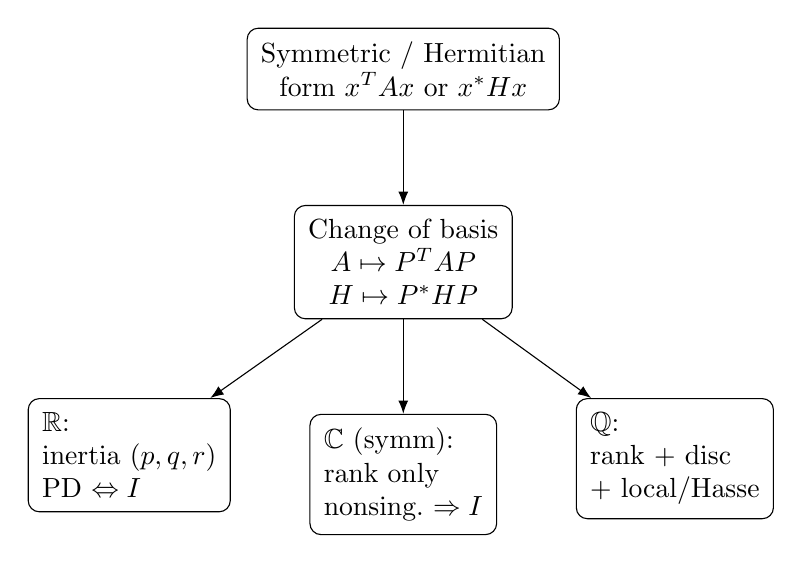
\begin{tikzpicture}[>=Latex, node distance=12mm]
		\node[draw, rounded corners, align=center, inner sep=5pt] (qf) {Symmetric / Hermitian\\ form $x^TAx$ or $x^*Hx$};
		\node[draw, rounded corners, align=center, inner sep=5pt, below=of qf] (change) {Change of basis\\ $A\mapsto P^TAP$\\ $H\mapsto P^*HP$};
		\node[draw, rounded corners, align=left, inner sep=5pt, below left=10mm and 8mm of change] (R) {$\mathbb R$:\\ inertia $(p,q,r)$\\ PD $\Leftrightarrow I$};
		\node[draw, rounded corners, align=left, inner sep=5pt, below=of change] (C) {$\mathbb C$ (symm):\\ rank only\\ nonsing.\ $\Rightarrow I$};
		\node[draw, rounded corners, align=left, inner sep=5pt, below right=10mm and 8mm of change] (Q) {$\mathbb Q$:\\ rank + disc\\ + local/Hasse};
		\draw[->] (qf) -- (change);
		\draw[->] (change) -- (R);
		\draw[->] (change) -- (C);
		\draw[->] (change) -- (Q);
	\end{tikzpicture}
\end{center}

% ---------------------------------------------------------

\subsubsection*{Chart C — Operator structure map (Problems 7--8, also 3)}

\begin{center}
	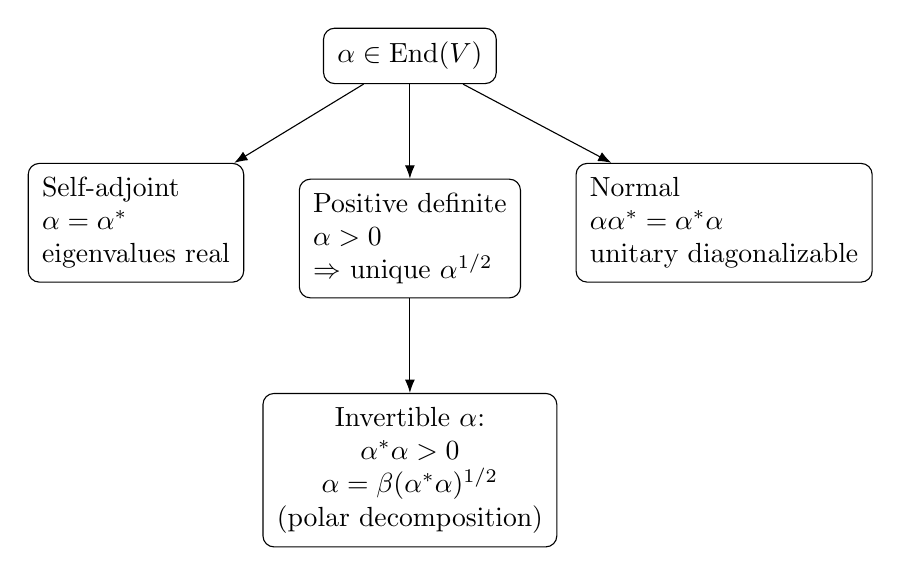
\begin{tikzpicture}[>=Latex, node distance=12mm]
		\node[draw, rounded corners, align=center, inner sep=5pt] (A) {$\alpha\in\mathrm{End}(V)$};
		\node[draw, rounded corners, align=left, inner sep=5pt, below left=10mm and 10mm of A] (sa)
		{Self-adjoint\\ $\alpha=\alpha^*$\\ eigenvalues real};
		\node[draw, rounded corners, align=left, inner sep=5pt, below=of A] (pd)
		{Positive definite\\ $\alpha>0$\\ $\Rightarrow$ unique $\alpha^{1/2}$};
		\node[draw, rounded corners, align=left, inner sep=5pt, below right=10mm and 10mm of A] (normal)
		{Normal\\ $\alpha\alpha^*=\alpha^*\alpha$\\ unitary diagonalizable};
		\node[draw, rounded corners, align=center, inner sep=5pt, below=of pd] (polar)
		{Invertible $\alpha$:\\ $\alpha^*\alpha>0$\\ $\alpha=\beta(\alpha^*\alpha)^{1/2}$\\ (polar decomposition)};
		\draw[->] (A) -- (sa);
		\draw[->] (A) -- (pd);
		\draw[->] (A) -- (normal);
		\draw[->] (pd) -- (polar);
	\end{tikzpicture}
\end{center}

% ---------------------------------------------------------

\subsubsection*{Chart D — Orthogonal polynomials pipeline (Problem 9)}

\begin{center}
	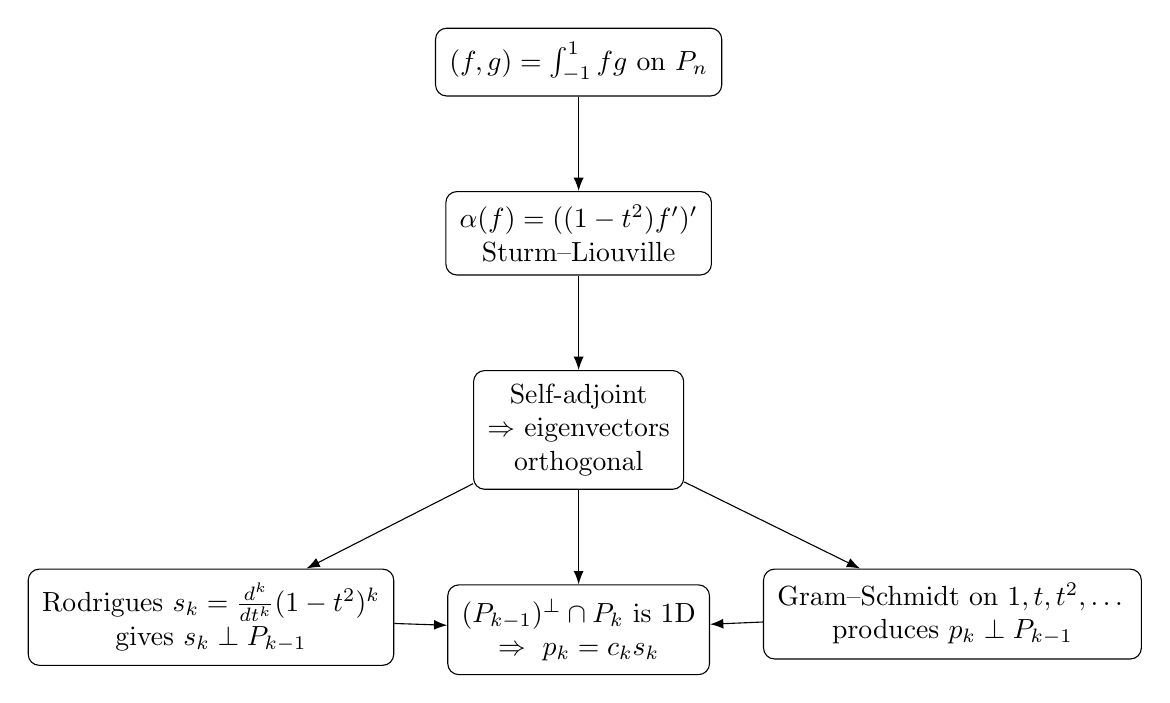
\begin{tikzpicture}[>=Latex, node distance=12mm]
		\node[draw, rounded corners, align=center, inner sep=5pt] (ip)
		{$(f,g)=\int_{-1}^1 fg$ on $P_n$};
		\node[draw, rounded corners, align=center, inner sep=5pt, below=of ip] (sl)
		{$\alpha(f)=((1-t^2)f')'$\\ Sturm--Liouville};
		\node[draw, rounded corners, align=center, inner sep=5pt, below=of sl] (sa)
		{Self-adjoint\\ $\Rightarrow$ eigenvectors\\ orthogonal};
		\node[draw, rounded corners, align=center, inner sep=5pt, below left=10mm and 10mm of sa] (rod)
		{Rodrigues $s_k=\frac{d^k}{dt^k}(1-t^2)^k$\\ gives $s_k\perp P_{k-1}$};
		\node[draw, rounded corners, align=center, inner sep=5pt, below right=10mm and 10mm of sa] (gs)
		{Gram--Schmidt on $1,t,t^2,\dots$\\ produces $p_k\perp P_{k-1}$};
		\node[draw, rounded corners, align=center, inner sep=5pt, below=of sa] (uniq)
		{$(P_{k-1})^\perp\cap P_k$ is 1D\\ $\Rightarrow\ p_k=c_k s_k$};
		\draw[->] (ip) -- (sl);
		\draw[->] (sl) -- (sa);
		\draw[->] (sa) -- (rod);
		\draw[->] (sa) -- (gs);
		\draw[->] (sa) -- (uniq);
		\draw[->] (rod) -- (uniq);
		\draw[->] (gs) -- (uniq);
	\end{tikzpicture}
\end{center}

% ---------------------------------------------------------

\subsubsection*{Chart E — Determinant as volume (Problem 12)}

\begin{center}
	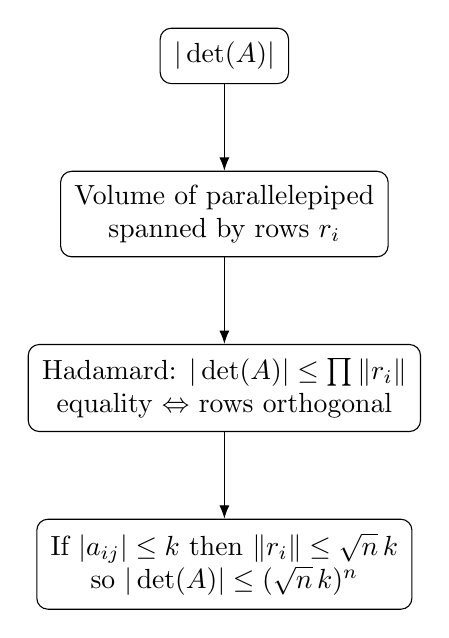
\begin{tikzpicture}[>=Latex, node distance=11mm]
		\node[draw, rounded corners, align=center, inner sep=5pt] (det)
		{$|\det(A)|$};
		\node[draw, rounded corners, align=center, inner sep=5pt, below=of det] (vol)
		{Volume of parallelepiped\\ spanned by rows $r_i$};
		\node[draw, rounded corners, align=center, inner sep=5pt, below=of vol] (had)
		{Hadamard: $|\det(A)|\le\prod\|r_i\|$\\ equality $\Leftrightarrow$ rows orthogonal};
		\node[draw, rounded corners, align=center, inner sep=5pt, below=of had] (bound)
		{If $|a_{ij}|\le k$ then $\|r_i\|\le\sqrt n\,k$\\ so $|\det(A)|\le (\sqrt n\,k)^n$};
		\draw[->] (det) -- (vol);
		\draw[->] (vol) -- (had);
		\draw[->] (had) -- (bound);
	\end{tikzpicture}
\end{center}

% ---------------------------------------------------------

\subsubsection*{Chart F — Two small “spectral patterns” (Problems 10 and 11)}

\begin{center}
	\renewcommand{\arraystretch}{1.25}
	\begin{tabular}{@{}p{7.0cm}p{6.5cm}@{}}
		\toprule
		\textbf{Cycle quadratic (Problem 10)} & \textbf{Symmetric finite order (Problem 11)}\\
		\midrule
		$Q$ circulant (neighbors on a cycle) &
		$S=S^T$ orthogonally diagonalizable\\
		Eigenvalues: $\lambda_m=\cos(2\pi m/n)$ &
		$S^k=I \Rightarrow \lambda_i^k=1$\\
		Constraint $\sum a_i=0$ removes mode $m=0$ &
		Real roots of unity $\Rightarrow \lambda_i\in\{\pm 1\}$\\
		Max on $\mathbf 1^\perp$: $\cos(2\pi/n)$ &
		Hence $S^2=I$\\
		\bottomrule
	\end{tabular}
\end{center}

	\end{document}

